\documentclass[twoside]{book}

% Packages required by doxygen
\usepackage{fixltx2e}
\usepackage{calc}
\usepackage{doxygen}
\usepackage[export]{adjustbox} % also loads graphicx
\usepackage{graphicx}
\usepackage[utf8]{inputenc}
\usepackage{makeidx}
\usepackage{multicol}
\usepackage{multirow}
\PassOptionsToPackage{warn}{textcomp}
\usepackage{textcomp}
\usepackage[nointegrals]{wasysym}
\usepackage[table]{xcolor}

% Font selection
\usepackage[T1]{fontenc}
\usepackage[scaled=.90]{helvet}
\usepackage{courier}
\usepackage{amssymb}
\usepackage{sectsty}
\renewcommand{\familydefault}{\sfdefault}
\allsectionsfont{%
  \fontseries{bc}\selectfont%
  \color{darkgray}%
}
\renewcommand{\DoxyLabelFont}{%
  \fontseries{bc}\selectfont%
  \color{darkgray}%
}
\newcommand{\+}{\discretionary{\mbox{\scriptsize$\hookleftarrow$}}{}{}}

% Page & text layout
\usepackage{geometry}
\geometry{%
  a4paper,%
  top=2.5cm,%
  bottom=2.5cm,%
  left=2.5cm,%
  right=2.5cm%
}
\tolerance=750
\hfuzz=15pt
\hbadness=750
\setlength{\emergencystretch}{15pt}
\setlength{\parindent}{0cm}
\setlength{\parskip}{0.2cm}
\makeatletter
\renewcommand{\paragraph}{%
  \@startsection{paragraph}{4}{0ex}{-1.0ex}{1.0ex}{%
    \normalfont\normalsize\bfseries\SS@parafont%
  }%
}
\renewcommand{\subparagraph}{%
  \@startsection{subparagraph}{5}{0ex}{-1.0ex}{1.0ex}{%
    \normalfont\normalsize\bfseries\SS@subparafont%
  }%
}
\makeatother

% Headers & footers
\usepackage{fancyhdr}
\pagestyle{fancyplain}
\fancyhead[LE]{\fancyplain{}{\bfseries\thepage}}
\fancyhead[CE]{\fancyplain{}{}}
\fancyhead[RE]{\fancyplain{}{\bfseries\leftmark}}
\fancyhead[LO]{\fancyplain{}{\bfseries\rightmark}}
\fancyhead[CO]{\fancyplain{}{}}
\fancyhead[RO]{\fancyplain{}{\bfseries\thepage}}
\fancyfoot[LE]{\fancyplain{}{}}
\fancyfoot[CE]{\fancyplain{}{}}
\fancyfoot[RE]{\fancyplain{}{\bfseries\scriptsize Generated on Mon Jun 15 2015 11\+:06\+:51 for N\+N\+T\+Lib by Doxygen }}
\fancyfoot[LO]{\fancyplain{}{\bfseries\scriptsize Generated on Mon Jun 15 2015 11\+:06\+:51 for N\+N\+T\+Lib by Doxygen }}
\fancyfoot[CO]{\fancyplain{}{}}
\fancyfoot[RO]{\fancyplain{}{}}
\renewcommand{\footrulewidth}{0.4pt}
\renewcommand{\chaptermark}[1]{%
  \markboth{#1}{}%
}
\renewcommand{\sectionmark}[1]{%
  \markright{\thesection\ #1}%
}

% Indices & bibliography
\usepackage{natbib}
\usepackage[titles]{tocloft}
\setcounter{tocdepth}{3}
\setcounter{secnumdepth}{5}
\makeindex

% Hyperlinks (required, but should be loaded last)
\usepackage{ifpdf}
\ifpdf
  \usepackage[pdftex,pagebackref=true]{hyperref}
\else
  \usepackage[ps2pdf,pagebackref=true]{hyperref}
\fi
\hypersetup{%
  colorlinks=true,%
  linkcolor=blue,%
  citecolor=blue,%
  unicode%
}

% Custom commands
\newcommand{\clearemptydoublepage}{%
  \newpage{\pagestyle{empty}\cleardoublepage}%
}


%===== C O N T E N T S =====

\begin{document}

% Titlepage & ToC
\hypersetup{pageanchor=false,
             bookmarks=true,
             bookmarksnumbered=true,
             pdfencoding=unicode
            }
\pagenumbering{roman}
\begin{titlepage}
\vspace*{7cm}
\begin{center}%
{\Large N\+N\+T\+Lib }\\
\vspace*{1cm}
{\large Generated by Doxygen 1.8.9.1}\\
\vspace*{0.5cm}
{\small Mon Jun 15 2015 11:06:51}\\
\end{center}
\end{titlepage}
\clearemptydoublepage
\tableofcontents
\clearemptydoublepage
\pagenumbering{arabic}
\hypersetup{pageanchor=true}

%--- Begin generated contents ---
\chapter{Hierarchical Index}
\section{Class Hierarchy}
This inheritance list is sorted roughly, but not completely, alphabetically\+:\begin{DoxyCompactList}
\item \contentsline{section}{Config\+Base}{\pageref{class_config_base}}{}
\begin{DoxyCompactList}
\item \contentsline{section}{Backpropagation\+Config}{\pageref{class_backpropagation_config}}{}
\item \contentsline{section}{Contrastive\+Divergence\+Config}{\pageref{class_contrastive_divergence_config}}{}
\item \contentsline{section}{Genetic\+Algorithm\+Config}{\pageref{class_genetic_algorithm_config}}{}
\item \contentsline{section}{Neural\+Network\+Config}{\pageref{class_neural_network_config}}{}
\end{DoxyCompactList}
\item \contentsline{section}{N\+N\+T\+Lib\+:\+:Data\+Container}{\pageref{class_n_n_t_lib_1_1_data_container}}{}
\item \contentsline{section}{N\+N\+T\+Lib\+:\+:Layer}{\pageref{class_n_n_t_lib_1_1_layer}}{}
\begin{DoxyCompactList}
\item \contentsline{section}{N\+N\+T\+Lib\+:\+:D\+B\+N\+Layer}{\pageref{class_n_n_t_lib_1_1_d_b_n_layer}}{}
\end{DoxyCompactList}
\item \contentsline{section}{N\+N\+T\+Lib\+:\+:Neural\+Network}{\pageref{class_n_n_t_lib_1_1_neural_network}}{}
\begin{DoxyCompactList}
\item \contentsline{section}{N\+N\+T\+Lib\+:\+:Deep\+Belief\+Net}{\pageref{class_n_n_t_lib_1_1_deep_belief_net}}{}
\end{DoxyCompactList}
\item \contentsline{section}{N\+N\+T\+Lib\+:\+:Neuron}{\pageref{class_n_n_t_lib_1_1_neuron}}{}
\begin{DoxyCompactList}
\item \contentsline{section}{N\+N\+T\+Lib\+:\+:D\+B\+N\+Neuron}{\pageref{class_n_n_t_lib_1_1_d_b_n_neuron}}{}
\end{DoxyCompactList}
\item \contentsline{section}{N\+N\+T\+Lib\+:\+:Trainer\+Base}{\pageref{class_n_n_t_lib_1_1_trainer_base}}{}
\begin{DoxyCompactList}
\item \contentsline{section}{N\+N\+T\+Lib\+:\+:Backpropagation}{\pageref{class_n_n_t_lib_1_1_backpropagation}}{}
\item \contentsline{section}{N\+N\+T\+Lib\+:\+:Contrastive\+Divergence}{\pageref{class_n_n_t_lib_1_1_contrastive_divergence}}{}
\item \contentsline{section}{N\+N\+T\+Lib\+:\+:Genetic\+Algorithm}{\pageref{class_n_n_t_lib_1_1_genetic_algorithm}}{}
\end{DoxyCompactList}
\item \contentsline{section}{N\+N\+T\+Lib\+:\+:Training\+Measure}{\pageref{struct_n_n_t_lib_1_1_training_measure}}{}
\end{DoxyCompactList}

\chapter{Class Index}
\section{Class List}
Here are the classes, structs, unions and interfaces with brief descriptions\+:\begin{DoxyCompactList}
\item\contentsline{section}{\hyperlink{class_n_n_t_lib_1_1_backpropagation}{N\+N\+T\+Lib\+::\+Backpropagation} }{\pageref{class_n_n_t_lib_1_1_backpropagation}}{}
\item\contentsline{section}{\hyperlink{class_backpropagation_config}{Backpropagation\+Config} }{\pageref{class_backpropagation_config}}{}
\item\contentsline{section}{\hyperlink{class_config_base}{Config\+Base} }{\pageref{class_config_base}}{}
\item\contentsline{section}{\hyperlink{class_n_n_t_lib_1_1_contrastive_divergence}{N\+N\+T\+Lib\+::\+Contrastive\+Divergence} }{\pageref{class_n_n_t_lib_1_1_contrastive_divergence}}{}
\item\contentsline{section}{\hyperlink{class_contrastive_divergence_config}{Contrastive\+Divergence\+Config} }{\pageref{class_contrastive_divergence_config}}{}
\item\contentsline{section}{\hyperlink{class_n_n_t_lib_1_1_data_container}{N\+N\+T\+Lib\+::\+Data\+Container} }{\pageref{class_n_n_t_lib_1_1_data_container}}{}
\item\contentsline{section}{\hyperlink{class_n_n_t_lib_1_1_d_b_n_layer}{N\+N\+T\+Lib\+::\+D\+B\+N\+Layer} }{\pageref{class_n_n_t_lib_1_1_d_b_n_layer}}{}
\item\contentsline{section}{\hyperlink{class_n_n_t_lib_1_1_d_b_n_neuron}{N\+N\+T\+Lib\+::\+D\+B\+N\+Neuron} }{\pageref{class_n_n_t_lib_1_1_d_b_n_neuron}}{}
\item\contentsline{section}{\hyperlink{class_n_n_t_lib_1_1_deep_belief_net}{N\+N\+T\+Lib\+::\+Deep\+Belief\+Net} }{\pageref{class_n_n_t_lib_1_1_deep_belief_net}}{}
\item\contentsline{section}{\hyperlink{class_n_n_t_lib_1_1_genetic_algorithm}{N\+N\+T\+Lib\+::\+Genetic\+Algorithm} }{\pageref{class_n_n_t_lib_1_1_genetic_algorithm}}{}
\item\contentsline{section}{\hyperlink{class_genetic_algorithm_config}{Genetic\+Algorithm\+Config} }{\pageref{class_genetic_algorithm_config}}{}
\item\contentsline{section}{\hyperlink{class_n_n_t_lib_1_1_layer}{N\+N\+T\+Lib\+::\+Layer} }{\pageref{class_n_n_t_lib_1_1_layer}}{}
\item\contentsline{section}{\hyperlink{class_n_n_t_lib_1_1_neural_network}{N\+N\+T\+Lib\+::\+Neural\+Network} }{\pageref{class_n_n_t_lib_1_1_neural_network}}{}
\item\contentsline{section}{\hyperlink{class_neural_network_config}{Neural\+Network\+Config} }{\pageref{class_neural_network_config}}{}
\item\contentsline{section}{\hyperlink{class_n_n_t_lib_1_1_neuron}{N\+N\+T\+Lib\+::\+Neuron} }{\pageref{class_n_n_t_lib_1_1_neuron}}{}
\item\contentsline{section}{\hyperlink{class_n_n_t_lib_1_1_trainer_base}{N\+N\+T\+Lib\+::\+Trainer\+Base} }{\pageref{class_n_n_t_lib_1_1_trainer_base}}{}
\item\contentsline{section}{\hyperlink{struct_n_n_t_lib_1_1_training_measure}{N\+N\+T\+Lib\+::\+Training\+Measure} }{\pageref{struct_n_n_t_lib_1_1_training_measure}}{}
\end{DoxyCompactList}

\chapter{Class Documentation}
\hypertarget{class_n_n_t_lib_1_1_backpropagation}{}\section{N\+N\+T\+Lib\+:\+:Backpropagation Class Reference}
\label{class_n_n_t_lib_1_1_backpropagation}\index{N\+N\+T\+Lib\+::\+Backpropagation@{N\+N\+T\+Lib\+::\+Backpropagation}}


Inheritance diagram for N\+N\+T\+Lib\+:\+:Backpropagation\+:\nopagebreak
\begin{figure}[H]
\begin{center}
\leavevmode
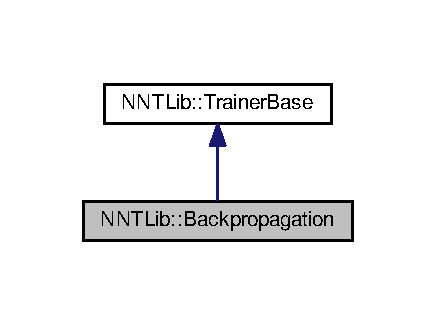
\includegraphics[width=209pt]{class_n_n_t_lib_1_1_backpropagation__inherit__graph}
\end{center}
\end{figure}


Collaboration diagram for N\+N\+T\+Lib\+:\+:Backpropagation\+:\nopagebreak
\begin{figure}[H]
\begin{center}
\leavevmode
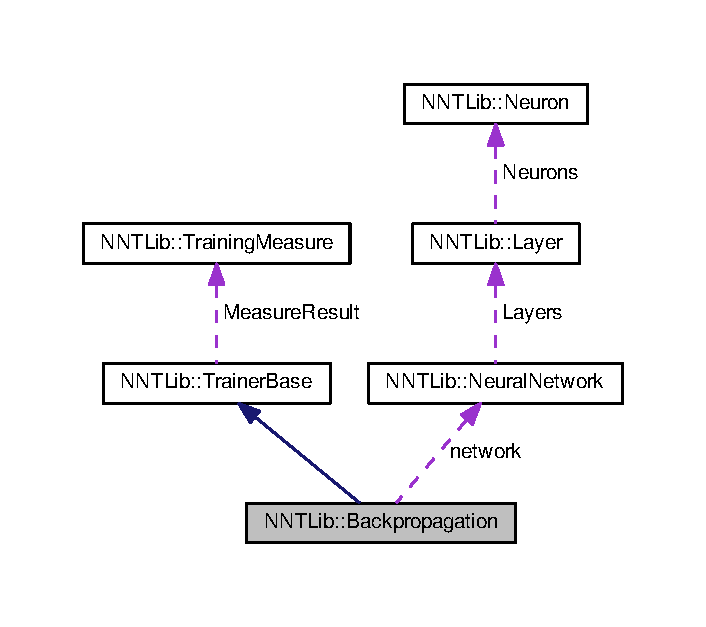
\includegraphics[width=339pt]{class_n_n_t_lib_1_1_backpropagation__coll__graph}
\end{center}
\end{figure}
\subsection*{Public Member Functions}
\begin{DoxyCompactItemize}
\item 
\hyperlink{class_n_n_t_lib_1_1_backpropagation_afadd50e1e66fb044a6999ec5094ca1af}{Backpropagation} (\hyperlink{class_n_n_t_lib_1_1_neural_network}{Neural\+Network} \&net)
\begin{DoxyCompactList}\small\item\em Initializes a new instance of the \hyperlink{class_n_n_t_lib_1_1_backpropagation}{Backpropagation} class. \end{DoxyCompactList}\item 
\hyperlink{class_n_n_t_lib_1_1_backpropagation_a35dbdb3ee50f6edc952ee23c35d79eee}{$\sim$\+Backpropagation} ()
\begin{DoxyCompactList}\small\item\em Finalizes an instance of the \hyperlink{class_n_n_t_lib_1_1_backpropagation}{Backpropagation} class. \end{DoxyCompactList}\item 
void \hyperlink{class_n_n_t_lib_1_1_backpropagation_a1043af2261f85a391ba3baccc1bc8b4b}{Train} (const \hyperlink{class_n_n_t_lib_1_1_data_container}{Data\+Container} \&container, const double learn\+Rate, const int max\+Loop\+Count, const double momentum=0, int minibatch\+Size=1, const double error\+Threshold=0, const double decay\+Rate=0)
\begin{DoxyCompactList}\small\item\em Trains the specified container. \end{DoxyCompactList}\end{DoxyCompactItemize}
\subsection*{Public Attributes}
\begin{DoxyCompactItemize}
\item 
\hyperlink{class_n_n_t_lib_1_1_neural_network}{Neural\+Network} $\ast$ \hyperlink{class_n_n_t_lib_1_1_backpropagation_af439beac84eedecfcdd2eb0c9ff98c5a}{network}
\begin{DoxyCompactList}\small\item\em The network \end{DoxyCompactList}\end{DoxyCompactItemize}
\subsection*{Additional Inherited Members}


\subsection{Constructor \& Destructor Documentation}
\hypertarget{class_n_n_t_lib_1_1_backpropagation_afadd50e1e66fb044a6999ec5094ca1af}{}\index{N\+N\+T\+Lib\+::\+Backpropagation@{N\+N\+T\+Lib\+::\+Backpropagation}!Backpropagation@{Backpropagation}}
\index{Backpropagation@{Backpropagation}!N\+N\+T\+Lib\+::\+Backpropagation@{N\+N\+T\+Lib\+::\+Backpropagation}}
\subsubsection[{Backpropagation}]{\setlength{\rightskip}{0pt plus 5cm}N\+N\+T\+Lib\+::\+Backpropagation\+::\+Backpropagation (
\begin{DoxyParamCaption}
\item[{{\bf Neural\+Network} \&}]{net}
\end{DoxyParamCaption}
)}\label{class_n_n_t_lib_1_1_backpropagation_afadd50e1e66fb044a6999ec5094ca1af}


Initializes a new instance of the \hyperlink{class_n_n_t_lib_1_1_backpropagation}{Backpropagation} class. 


\begin{DoxyParams}{Parameters}
{\em net} & The net.\\
\hline
\end{DoxyParams}
\hypertarget{class_n_n_t_lib_1_1_backpropagation_a35dbdb3ee50f6edc952ee23c35d79eee}{}\index{N\+N\+T\+Lib\+::\+Backpropagation@{N\+N\+T\+Lib\+::\+Backpropagation}!````~Backpropagation@{$\sim$\+Backpropagation}}
\index{````~Backpropagation@{$\sim$\+Backpropagation}!N\+N\+T\+Lib\+::\+Backpropagation@{N\+N\+T\+Lib\+::\+Backpropagation}}
\subsubsection[{$\sim$\+Backpropagation}]{\setlength{\rightskip}{0pt plus 5cm}N\+N\+T\+Lib\+::\+Backpropagation\+::$\sim$\+Backpropagation (
\begin{DoxyParamCaption}
{}
\end{DoxyParamCaption}
)}\label{class_n_n_t_lib_1_1_backpropagation_a35dbdb3ee50f6edc952ee23c35d79eee}


Finalizes an instance of the \hyperlink{class_n_n_t_lib_1_1_backpropagation}{Backpropagation} class. 



\subsection{Member Function Documentation}
\hypertarget{class_n_n_t_lib_1_1_backpropagation_a1043af2261f85a391ba3baccc1bc8b4b}{}\index{N\+N\+T\+Lib\+::\+Backpropagation@{N\+N\+T\+Lib\+::\+Backpropagation}!Train@{Train}}
\index{Train@{Train}!N\+N\+T\+Lib\+::\+Backpropagation@{N\+N\+T\+Lib\+::\+Backpropagation}}
\subsubsection[{Train}]{\setlength{\rightskip}{0pt plus 5cm}void N\+N\+T\+Lib\+::\+Backpropagation\+::\+Train (
\begin{DoxyParamCaption}
\item[{const {\bf Data\+Container} \&}]{container, }
\item[{const double}]{learn\+Rate, }
\item[{const int}]{max\+Loop\+Count, }
\item[{const double}]{momentum = {\ttfamily 0}, }
\item[{int}]{minibatch\+Size = {\ttfamily 1}, }
\item[{const double}]{error\+Threshold = {\ttfamily 0}, }
\item[{const double}]{decay\+Rate = {\ttfamily 0}}
\end{DoxyParamCaption}
)}\label{class_n_n_t_lib_1_1_backpropagation_a1043af2261f85a391ba3baccc1bc8b4b}


Trains the specified container. 


\begin{DoxyParams}{Parameters}
{\em container} & The container.\\
\hline
{\em learn\+Rate} & The learn rate.\\
\hline
{\em max\+Loop\+Count} & The maximum loop count.\\
\hline
{\em momentum} & The momentum.\\
\hline
{\em minibatch\+Size} & Size of the batch.\\
\hline
{\em error\+Threshold} & The error threshold.\\
\hline
{\em decay\+Rate} & The decay rate.\\
\hline
\end{DoxyParams}


\subsection{Member Data Documentation}
\hypertarget{class_n_n_t_lib_1_1_backpropagation_af439beac84eedecfcdd2eb0c9ff98c5a}{}\index{N\+N\+T\+Lib\+::\+Backpropagation@{N\+N\+T\+Lib\+::\+Backpropagation}!network@{network}}
\index{network@{network}!N\+N\+T\+Lib\+::\+Backpropagation@{N\+N\+T\+Lib\+::\+Backpropagation}}
\subsubsection[{network}]{\setlength{\rightskip}{0pt plus 5cm}{\bf Neural\+Network}$\ast$ N\+N\+T\+Lib\+::\+Backpropagation\+::network}\label{class_n_n_t_lib_1_1_backpropagation_af439beac84eedecfcdd2eb0c9ff98c5a}


The network 



The documentation for this class was generated from the following files\+:\begin{DoxyCompactItemize}
\item 
N\+N\+T\+Lib/Backpropagation.\+h\item 
N\+N\+T\+Lib/Backpropagation.\+cpp\end{DoxyCompactItemize}

\hypertarget{class_backpropagation_config}{}\section{Backpropagation\+Config Class Reference}
\label{class_backpropagation_config}\index{Backpropagation\+Config@{Backpropagation\+Config}}


Inheritance diagram for Backpropagation\+Config\+:\nopagebreak
\begin{figure}[H]
\begin{center}
\leavevmode
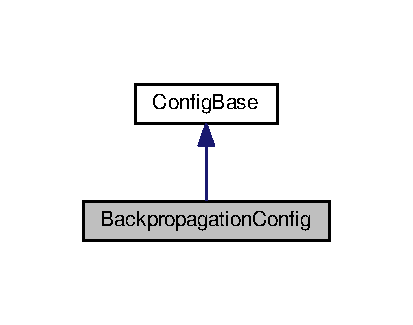
\includegraphics[width=198pt]{class_backpropagation_config__inherit__graph}
\end{center}
\end{figure}


Collaboration diagram for Backpropagation\+Config\+:\nopagebreak
\begin{figure}[H]
\begin{center}
\leavevmode
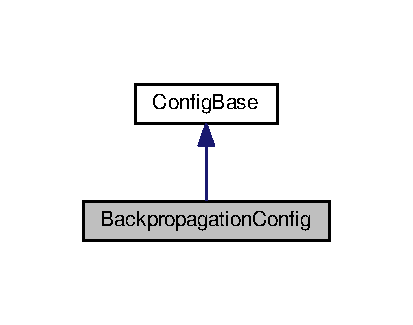
\includegraphics[width=198pt]{class_backpropagation_config__coll__graph}
\end{center}
\end{figure}
\subsection*{Public Member Functions}
\begin{DoxyCompactItemize}
\item 
\hyperlink{class_backpropagation_config_a52af8244ad7e5554ebbeedea47ddff2a}{Backpropagation\+Config} ()
\begin{DoxyCompactList}\small\item\em Initializes a new instance of the \hyperlink{class_backpropagation_config}{Backpropagation\+Config} class. \end{DoxyCompactList}\item 
void \hyperlink{class_backpropagation_config_aa9e60f952307833c8ebf84d1bce21ea0}{Print\+Data} ()
\begin{DoxyCompactList}\small\item\em Prints the data. \end{DoxyCompactList}\item 
bool \hyperlink{class_backpropagation_config_a64c50d10f6091ea19a2ec5db6481437e}{Is\+Config\+Valid} ()
\begin{DoxyCompactList}\small\item\em Determines whether \mbox{[}is configuration valid\mbox{]}. \end{DoxyCompactList}\end{DoxyCompactItemize}
\subsection*{Public Attributes}
\begin{DoxyCompactItemize}
\item 
double \hyperlink{class_backpropagation_config_a5c50a9fcfd1a06421c6a0ae3c70a3a55}{Error\+Threshold}
\begin{DoxyCompactList}\small\item\em The error threshold \end{DoxyCompactList}\item 
int \hyperlink{class_backpropagation_config_a5f13785a5b5451815c46fa475af82fac}{Max\+Loop\+Count}
\begin{DoxyCompactList}\small\item\em The maximum loop count \end{DoxyCompactList}\item 
int \hyperlink{class_backpropagation_config_a44b2e5b4975e49fbcd51a241575904d4}{Batch\+Size}
\begin{DoxyCompactList}\small\item\em The batch size \end{DoxyCompactList}\item 
double \hyperlink{class_backpropagation_config_a79edf18125f39372ef11a0f087e734ab}{Alpha}
\begin{DoxyCompactList}\small\item\em The alpha \end{DoxyCompactList}\item 
double \hyperlink{class_backpropagation_config_a8b108e7cddcbf2cc103b813708057487}{Momentum}
\begin{DoxyCompactList}\small\item\em The momentum \end{DoxyCompactList}\item 
double \hyperlink{class_backpropagation_config_a28853172211206ad458fbc72cabf252e}{Decay\+Rate}
\begin{DoxyCompactList}\small\item\em The decay rate \end{DoxyCompactList}\end{DoxyCompactItemize}
\subsection*{Protected Member Functions}
\begin{DoxyCompactItemize}
\item 
void \hyperlink{class_backpropagation_config_a375c3f21a8a3e3f834ebd098d82d1f97}{Handle\+Name\+Value} (std\+::string name, std\+::string value)
\begin{DoxyCompactList}\small\item\em Handles the name value. \end{DoxyCompactList}\end{DoxyCompactItemize}


\subsection{Constructor \& Destructor Documentation}
\hypertarget{class_backpropagation_config_a52af8244ad7e5554ebbeedea47ddff2a}{}\index{Backpropagation\+Config@{Backpropagation\+Config}!Backpropagation\+Config@{Backpropagation\+Config}}
\index{Backpropagation\+Config@{Backpropagation\+Config}!Backpropagation\+Config@{Backpropagation\+Config}}
\subsubsection[{Backpropagation\+Config}]{\setlength{\rightskip}{0pt plus 5cm}Backpropagation\+Config\+::\+Backpropagation\+Config (
\begin{DoxyParamCaption}
{}
\end{DoxyParamCaption}
)}\label{class_backpropagation_config_a52af8244ad7e5554ebbeedea47ddff2a}


Initializes a new instance of the \hyperlink{class_backpropagation_config}{Backpropagation\+Config} class. 



\subsection{Member Function Documentation}
\hypertarget{class_backpropagation_config_a375c3f21a8a3e3f834ebd098d82d1f97}{}\index{Backpropagation\+Config@{Backpropagation\+Config}!Handle\+Name\+Value@{Handle\+Name\+Value}}
\index{Handle\+Name\+Value@{Handle\+Name\+Value}!Backpropagation\+Config@{Backpropagation\+Config}}
\subsubsection[{Handle\+Name\+Value}]{\setlength{\rightskip}{0pt plus 5cm}void Backpropagation\+Config\+::\+Handle\+Name\+Value (
\begin{DoxyParamCaption}
\item[{std\+::string}]{name, }
\item[{std\+::string}]{value}
\end{DoxyParamCaption}
)\hspace{0.3cm}{\ttfamily [protected]}, {\ttfamily [virtual]}}\label{class_backpropagation_config_a375c3f21a8a3e3f834ebd098d82d1f97}


Handles the name value. 


\begin{DoxyParams}{Parameters}
{\em name} & The name.\\
\hline
{\em value} & The value.\\
\hline
\end{DoxyParams}


Implements \hyperlink{class_config_base}{Config\+Base}.

\hypertarget{class_backpropagation_config_a64c50d10f6091ea19a2ec5db6481437e}{}\index{Backpropagation\+Config@{Backpropagation\+Config}!Is\+Config\+Valid@{Is\+Config\+Valid}}
\index{Is\+Config\+Valid@{Is\+Config\+Valid}!Backpropagation\+Config@{Backpropagation\+Config}}
\subsubsection[{Is\+Config\+Valid}]{\setlength{\rightskip}{0pt plus 5cm}bool Backpropagation\+Config\+::\+Is\+Config\+Valid (
\begin{DoxyParamCaption}
{}
\end{DoxyParamCaption}
)\hspace{0.3cm}{\ttfamily [virtual]}}\label{class_backpropagation_config_a64c50d10f6091ea19a2ec5db6481437e}


Determines whether \mbox{[}is configuration valid\mbox{]}. 

\begin{DoxyReturn}{Returns}

\end{DoxyReturn}


Implements \hyperlink{class_config_base}{Config\+Base}.

\hypertarget{class_backpropagation_config_aa9e60f952307833c8ebf84d1bce21ea0}{}\index{Backpropagation\+Config@{Backpropagation\+Config}!Print\+Data@{Print\+Data}}
\index{Print\+Data@{Print\+Data}!Backpropagation\+Config@{Backpropagation\+Config}}
\subsubsection[{Print\+Data}]{\setlength{\rightskip}{0pt plus 5cm}void Backpropagation\+Config\+::\+Print\+Data (
\begin{DoxyParamCaption}
{}
\end{DoxyParamCaption}
)\hspace{0.3cm}{\ttfamily [virtual]}}\label{class_backpropagation_config_aa9e60f952307833c8ebf84d1bce21ea0}


Prints the data. 



Implements \hyperlink{class_config_base}{Config\+Base}.



\subsection{Member Data Documentation}
\hypertarget{class_backpropagation_config_a79edf18125f39372ef11a0f087e734ab}{}\index{Backpropagation\+Config@{Backpropagation\+Config}!Alpha@{Alpha}}
\index{Alpha@{Alpha}!Backpropagation\+Config@{Backpropagation\+Config}}
\subsubsection[{Alpha}]{\setlength{\rightskip}{0pt plus 5cm}double Backpropagation\+Config\+::\+Alpha}\label{class_backpropagation_config_a79edf18125f39372ef11a0f087e734ab}


The alpha 

\hypertarget{class_backpropagation_config_a44b2e5b4975e49fbcd51a241575904d4}{}\index{Backpropagation\+Config@{Backpropagation\+Config}!Batch\+Size@{Batch\+Size}}
\index{Batch\+Size@{Batch\+Size}!Backpropagation\+Config@{Backpropagation\+Config}}
\subsubsection[{Batch\+Size}]{\setlength{\rightskip}{0pt plus 5cm}int Backpropagation\+Config\+::\+Batch\+Size}\label{class_backpropagation_config_a44b2e5b4975e49fbcd51a241575904d4}


The batch size 

\hypertarget{class_backpropagation_config_a28853172211206ad458fbc72cabf252e}{}\index{Backpropagation\+Config@{Backpropagation\+Config}!Decay\+Rate@{Decay\+Rate}}
\index{Decay\+Rate@{Decay\+Rate}!Backpropagation\+Config@{Backpropagation\+Config}}
\subsubsection[{Decay\+Rate}]{\setlength{\rightskip}{0pt plus 5cm}double Backpropagation\+Config\+::\+Decay\+Rate}\label{class_backpropagation_config_a28853172211206ad458fbc72cabf252e}


The decay rate 

\hypertarget{class_backpropagation_config_a5c50a9fcfd1a06421c6a0ae3c70a3a55}{}\index{Backpropagation\+Config@{Backpropagation\+Config}!Error\+Threshold@{Error\+Threshold}}
\index{Error\+Threshold@{Error\+Threshold}!Backpropagation\+Config@{Backpropagation\+Config}}
\subsubsection[{Error\+Threshold}]{\setlength{\rightskip}{0pt plus 5cm}double Backpropagation\+Config\+::\+Error\+Threshold}\label{class_backpropagation_config_a5c50a9fcfd1a06421c6a0ae3c70a3a55}


The error threshold 

\hypertarget{class_backpropagation_config_a5f13785a5b5451815c46fa475af82fac}{}\index{Backpropagation\+Config@{Backpropagation\+Config}!Max\+Loop\+Count@{Max\+Loop\+Count}}
\index{Max\+Loop\+Count@{Max\+Loop\+Count}!Backpropagation\+Config@{Backpropagation\+Config}}
\subsubsection[{Max\+Loop\+Count}]{\setlength{\rightskip}{0pt plus 5cm}int Backpropagation\+Config\+::\+Max\+Loop\+Count}\label{class_backpropagation_config_a5f13785a5b5451815c46fa475af82fac}


The maximum loop count 

\hypertarget{class_backpropagation_config_a8b108e7cddcbf2cc103b813708057487}{}\index{Backpropagation\+Config@{Backpropagation\+Config}!Momentum@{Momentum}}
\index{Momentum@{Momentum}!Backpropagation\+Config@{Backpropagation\+Config}}
\subsubsection[{Momentum}]{\setlength{\rightskip}{0pt plus 5cm}double Backpropagation\+Config\+::\+Momentum}\label{class_backpropagation_config_a8b108e7cddcbf2cc103b813708057487}


The momentum 



The documentation for this class was generated from the following files\+:\begin{DoxyCompactItemize}
\item 
N\+N\+T\+Lib/Backpropagation\+Config.\+h\item 
N\+N\+T\+Lib/Backpropagation\+Config.\+cpp\end{DoxyCompactItemize}

\hypertarget{class_config_base}{}\section{Config\+Base Class Reference}
\label{class_config_base}\index{Config\+Base@{Config\+Base}}


Inheritance diagram for Config\+Base\+:\nopagebreak
\begin{figure}[H]
\begin{center}
\leavevmode
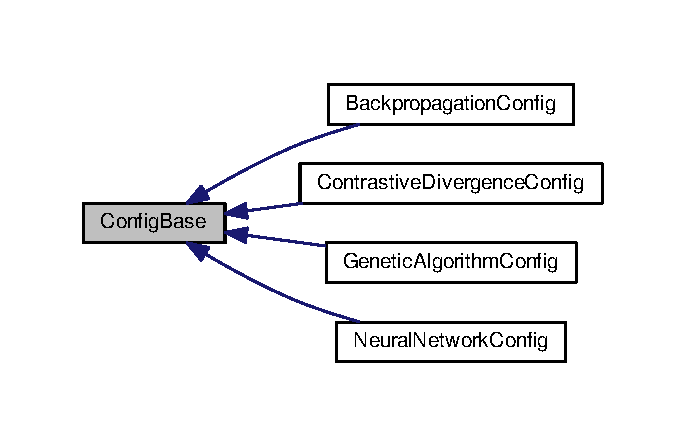
\includegraphics[width=329pt]{class_config_base__inherit__graph}
\end{center}
\end{figure}
\subsection*{Public Member Functions}
\begin{DoxyCompactItemize}
\item 
void \hyperlink{class_config_base_a2a1bfbf33daf2fb6b9f8cf9a059d68b7}{Load\+File} (const char $\ast$file)
\begin{DoxyCompactList}\small\item\em Loads the file. \end{DoxyCompactList}\item 
virtual \hyperlink{class_config_base_a429987eb53dd57fb0467501eb7a6ce80}{$\sim$\+Config\+Base} ()
\begin{DoxyCompactList}\small\item\em Finalizes an instance of the \hyperlink{class_config_base}{Config\+Base} class. \end{DoxyCompactList}\item 
\hypertarget{class_config_base_afd041dbca3845e8e7407f796bd882bdd}{}virtual void {\bfseries Print\+Data} ()=0\label{class_config_base_afd041dbca3845e8e7407f796bd882bdd}

\item 
\hypertarget{class_config_base_af05da2c1950ce4c30e6f16c3bf727a1a}{}virtual bool {\bfseries Is\+Config\+Valid} ()=0\label{class_config_base_af05da2c1950ce4c30e6f16c3bf727a1a}

\end{DoxyCompactItemize}
\subsection*{Protected Member Functions}
\begin{DoxyCompactItemize}
\item 
\hypertarget{class_config_base_a8c1a205fe3b3966eac5568bad8db9c88}{}virtual void {\bfseries Handle\+Name\+Value} (std\+::string name, std\+::string value)=0\label{class_config_base_a8c1a205fe3b3966eac5568bad8db9c88}

\end{DoxyCompactItemize}


\subsection{Constructor \& Destructor Documentation}
\hypertarget{class_config_base_a429987eb53dd57fb0467501eb7a6ce80}{}\index{Config\+Base@{Config\+Base}!````~Config\+Base@{$\sim$\+Config\+Base}}
\index{````~Config\+Base@{$\sim$\+Config\+Base}!Config\+Base@{Config\+Base}}
\subsubsection[{$\sim$\+Config\+Base}]{\setlength{\rightskip}{0pt plus 5cm}Config\+Base\+::$\sim$\+Config\+Base (
\begin{DoxyParamCaption}
{}
\end{DoxyParamCaption}
)\hspace{0.3cm}{\ttfamily [virtual]}}\label{class_config_base_a429987eb53dd57fb0467501eb7a6ce80}


Finalizes an instance of the \hyperlink{class_config_base}{Config\+Base} class. 



\subsection{Member Function Documentation}
\hypertarget{class_config_base_a2a1bfbf33daf2fb6b9f8cf9a059d68b7}{}\index{Config\+Base@{Config\+Base}!Load\+File@{Load\+File}}
\index{Load\+File@{Load\+File}!Config\+Base@{Config\+Base}}
\subsubsection[{Load\+File}]{\setlength{\rightskip}{0pt plus 5cm}void Config\+Base\+::\+Load\+File (
\begin{DoxyParamCaption}
\item[{const char $\ast$}]{file}
\end{DoxyParamCaption}
)}\label{class_config_base_a2a1bfbf33daf2fb6b9f8cf9a059d68b7}


Loads the file. 


\begin{DoxyParams}{Parameters}
{\em file} & The file.\\
\hline
\end{DoxyParams}


The documentation for this class was generated from the following files\+:\begin{DoxyCompactItemize}
\item 
N\+N\+T\+Lib/Config\+Base.\+h\item 
N\+N\+T\+Lib/Config\+Base.\+cpp\end{DoxyCompactItemize}

\hypertarget{class_n_n_t_lib_1_1_contrastive_divergence}{}\section{N\+N\+T\+Lib\+:\+:Contrastive\+Divergence Class Reference}
\label{class_n_n_t_lib_1_1_contrastive_divergence}\index{N\+N\+T\+Lib\+::\+Contrastive\+Divergence@{N\+N\+T\+Lib\+::\+Contrastive\+Divergence}}


Inheritance diagram for N\+N\+T\+Lib\+:\+:Contrastive\+Divergence\+:\nopagebreak
\begin{figure}[H]
\begin{center}
\leavevmode
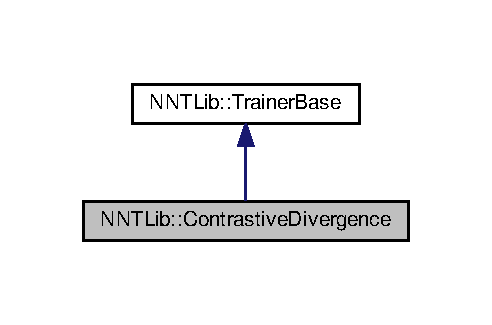
\includegraphics[width=236pt]{class_n_n_t_lib_1_1_contrastive_divergence__inherit__graph}
\end{center}
\end{figure}


Collaboration diagram for N\+N\+T\+Lib\+:\+:Contrastive\+Divergence\+:\nopagebreak
\begin{figure}[H]
\begin{center}
\leavevmode
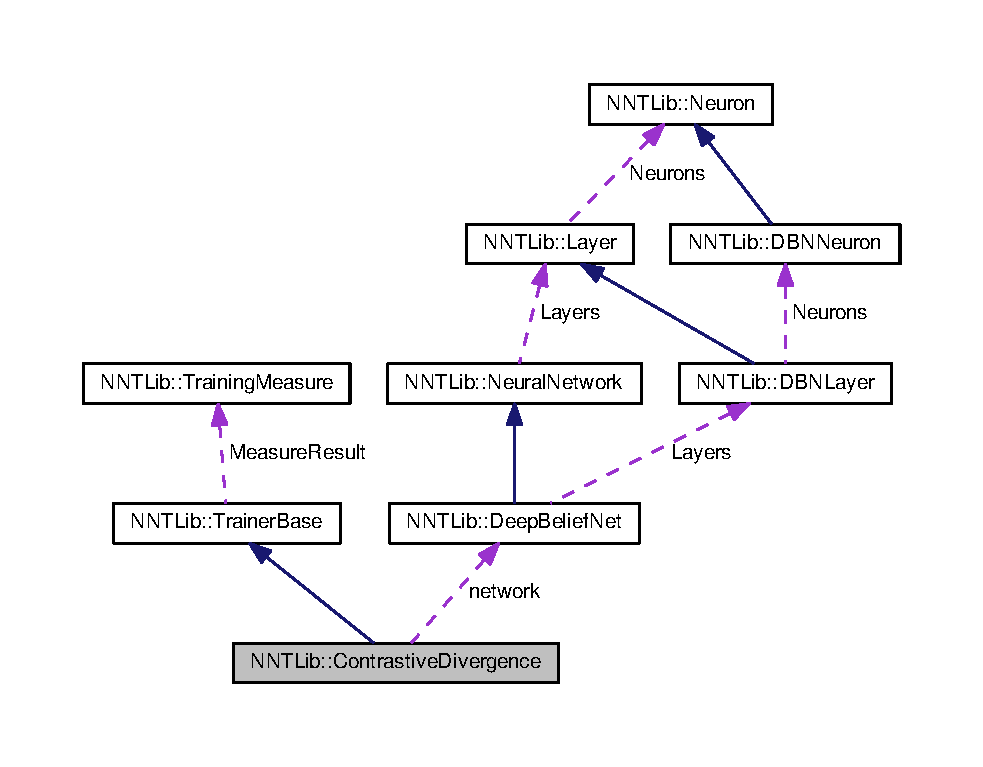
\includegraphics[width=350pt]{class_n_n_t_lib_1_1_contrastive_divergence__coll__graph}
\end{center}
\end{figure}
\subsection*{Public Member Functions}
\begin{DoxyCompactItemize}
\item 
\hypertarget{class_n_n_t_lib_1_1_contrastive_divergence_af8d48ef13d5e30cdde1372425230d82b}{}void {\bfseries Gibbs\+Sampling} (int gibbssteps, int d\+\_\+i)\label{class_n_n_t_lib_1_1_contrastive_divergence_af8d48ef13d5e30cdde1372425230d82b}

\item 
\hypertarget{class_n_n_t_lib_1_1_contrastive_divergence_a8d7e04a31fe118f4678c10a9dfd7876d}{}void {\bfseries Update\+Hidden\+Units} ()\label{class_n_n_t_lib_1_1_contrastive_divergence_a8d7e04a31fe118f4678c10a9dfd7876d}

\item 
\hypertarget{class_n_n_t_lib_1_1_contrastive_divergence_a3f66c00638df080d832bfd38219697b9}{}void {\bfseries Update\+Visible\+Units} ()\label{class_n_n_t_lib_1_1_contrastive_divergence_a3f66c00638df080d832bfd38219697b9}

\item 
\hypertarget{class_n_n_t_lib_1_1_contrastive_divergence_a5f8fe01e199eab56eec930ab6c313eb6}{}{\bfseries Contrastive\+Divergence} (\hyperlink{class_n_n_t_lib_1_1_deep_belief_net}{Deep\+Belief\+Net} \&net)\label{class_n_n_t_lib_1_1_contrastive_divergence_a5f8fe01e199eab56eec930ab6c313eb6}

\item 
\hypertarget{class_n_n_t_lib_1_1_contrastive_divergence_a479055ffdf7289c4726b73137afc287e}{}void {\bfseries Train} (const \hyperlink{class_n_n_t_lib_1_1_data_container}{Data\+Container} \&container, const double learn\+Rate, const int Epochs, int Batch\+Size=1, int gibbs=1)\label{class_n_n_t_lib_1_1_contrastive_divergence_a479055ffdf7289c4726b73137afc287e}

\end{DoxyCompactItemize}
\subsection*{Public Attributes}
\begin{DoxyCompactItemize}
\item 
\hyperlink{class_n_n_t_lib_1_1_deep_belief_net}{Deep\+Belief\+Net} $\ast$ \hyperlink{class_n_n_t_lib_1_1_contrastive_divergence_a922b07047f0dacb946fbbf3828484ad4}{network}
\begin{DoxyCompactList}\small\item\em The network \end{DoxyCompactList}\end{DoxyCompactItemize}
\subsection*{Additional Inherited Members}


\subsection{Member Data Documentation}
\hypertarget{class_n_n_t_lib_1_1_contrastive_divergence_a922b07047f0dacb946fbbf3828484ad4}{}\index{N\+N\+T\+Lib\+::\+Contrastive\+Divergence@{N\+N\+T\+Lib\+::\+Contrastive\+Divergence}!network@{network}}
\index{network@{network}!N\+N\+T\+Lib\+::\+Contrastive\+Divergence@{N\+N\+T\+Lib\+::\+Contrastive\+Divergence}}
\subsubsection[{network}]{\setlength{\rightskip}{0pt plus 5cm}{\bf Deep\+Belief\+Net}$\ast$ N\+N\+T\+Lib\+::\+Contrastive\+Divergence\+::network}\label{class_n_n_t_lib_1_1_contrastive_divergence_a922b07047f0dacb946fbbf3828484ad4}


The network 



The documentation for this class was generated from the following files\+:\begin{DoxyCompactItemize}
\item 
N\+N\+T\+Lib/Contrastive\+Divergence.\+h\item 
N\+N\+T\+Lib/Contrastive\+Divergence.\+cpp\end{DoxyCompactItemize}

\hypertarget{class_contrastive_divergence_config}{}\section{Contrastive\+Divergence\+Config Class Reference}
\label{class_contrastive_divergence_config}\index{Contrastive\+Divergence\+Config@{Contrastive\+Divergence\+Config}}


Inheritance diagram for Contrastive\+Divergence\+Config\+:\nopagebreak
\begin{figure}[H]
\begin{center}
\leavevmode
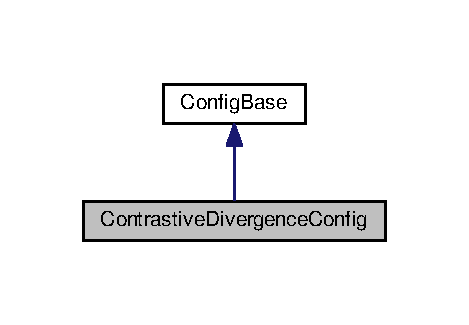
\includegraphics[width=225pt]{class_contrastive_divergence_config__inherit__graph}
\end{center}
\end{figure}


Collaboration diagram for Contrastive\+Divergence\+Config\+:\nopagebreak
\begin{figure}[H]
\begin{center}
\leavevmode
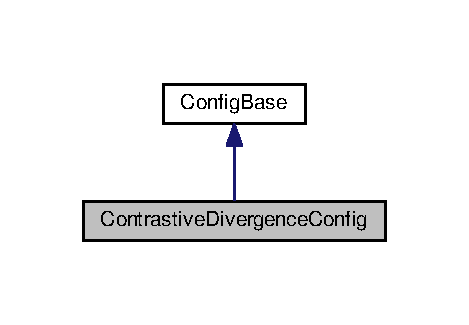
\includegraphics[width=225pt]{class_contrastive_divergence_config__coll__graph}
\end{center}
\end{figure}
\subsection*{Public Member Functions}
\begin{DoxyCompactItemize}
\item 
\hyperlink{class_contrastive_divergence_config_a7bdc6897aeb8e1ad3e09a92e62ec9e61}{Contrastive\+Divergence\+Config} ()
\begin{DoxyCompactList}\small\item\em Initializes a new instance of the \hyperlink{class_contrastive_divergence_config}{Contrastive\+Divergence\+Config} class. \end{DoxyCompactList}\item 
void \hyperlink{class_contrastive_divergence_config_ae9f613a4046f8545fedb37fe5a294c0e}{Print\+Data} ()
\begin{DoxyCompactList}\small\item\em Prints the data. \end{DoxyCompactList}\item 
bool \hyperlink{class_contrastive_divergence_config_ab168a8567c5309b0a61006747c4a44ce}{Is\+Config\+Valid} ()
\begin{DoxyCompactList}\small\item\em Determines whether \mbox{[}is configuration valid\mbox{]}. \end{DoxyCompactList}\end{DoxyCompactItemize}
\subsection*{Public Attributes}
\begin{DoxyCompactItemize}
\item 
int \hyperlink{class_contrastive_divergence_config_a9544c35ecb2c5adb8e51d12edc3c0510}{Gibbs\+Steps}
\begin{DoxyCompactList}\small\item\em The error threshold \end{DoxyCompactList}\item 
int \hyperlink{class_contrastive_divergence_config_ac8251503f35bac295b8b83220ace65fa}{Batch\+Size}
\begin{DoxyCompactList}\small\item\em The batch size \end{DoxyCompactList}\item 
double \hyperlink{class_contrastive_divergence_config_a826b90a2f85b952d7c633589b9574e52}{Learn\+Rate}
\begin{DoxyCompactList}\small\item\em The alpha \end{DoxyCompactList}\item 
\hypertarget{class_contrastive_divergence_config_a7c7c31e19877b3df6b38c896b74559b4}{}int {\bfseries Epochs}\label{class_contrastive_divergence_config_a7c7c31e19877b3df6b38c896b74559b4}

\end{DoxyCompactItemize}
\subsection*{Protected Member Functions}
\begin{DoxyCompactItemize}
\item 
void \hyperlink{class_contrastive_divergence_config_a9de17158dd8a544e591491aef5880bd5}{Handle\+Name\+Value} (std\+::string name, std\+::string value)
\begin{DoxyCompactList}\small\item\em Handles the name value. \end{DoxyCompactList}\end{DoxyCompactItemize}


\subsection{Constructor \& Destructor Documentation}
\hypertarget{class_contrastive_divergence_config_a7bdc6897aeb8e1ad3e09a92e62ec9e61}{}\index{Contrastive\+Divergence\+Config@{Contrastive\+Divergence\+Config}!Contrastive\+Divergence\+Config@{Contrastive\+Divergence\+Config}}
\index{Contrastive\+Divergence\+Config@{Contrastive\+Divergence\+Config}!Contrastive\+Divergence\+Config@{Contrastive\+Divergence\+Config}}
\subsubsection[{Contrastive\+Divergence\+Config}]{\setlength{\rightskip}{0pt plus 5cm}Contrastive\+Divergence\+Config\+::\+Contrastive\+Divergence\+Config (
\begin{DoxyParamCaption}
{}
\end{DoxyParamCaption}
)}\label{class_contrastive_divergence_config_a7bdc6897aeb8e1ad3e09a92e62ec9e61}


Initializes a new instance of the \hyperlink{class_contrastive_divergence_config}{Contrastive\+Divergence\+Config} class. 



\subsection{Member Function Documentation}
\hypertarget{class_contrastive_divergence_config_a9de17158dd8a544e591491aef5880bd5}{}\index{Contrastive\+Divergence\+Config@{Contrastive\+Divergence\+Config}!Handle\+Name\+Value@{Handle\+Name\+Value}}
\index{Handle\+Name\+Value@{Handle\+Name\+Value}!Contrastive\+Divergence\+Config@{Contrastive\+Divergence\+Config}}
\subsubsection[{Handle\+Name\+Value}]{\setlength{\rightskip}{0pt plus 5cm}void Contrastive\+Divergence\+Config\+::\+Handle\+Name\+Value (
\begin{DoxyParamCaption}
\item[{std\+::string}]{name, }
\item[{std\+::string}]{value}
\end{DoxyParamCaption}
)\hspace{0.3cm}{\ttfamily [protected]}, {\ttfamily [virtual]}}\label{class_contrastive_divergence_config_a9de17158dd8a544e591491aef5880bd5}


Handles the name value. 


\begin{DoxyParams}{Parameters}
{\em name} & The name.\\
\hline
{\em value} & The value.\\
\hline
\end{DoxyParams}


Implements \hyperlink{class_config_base}{Config\+Base}.

\hypertarget{class_contrastive_divergence_config_ab168a8567c5309b0a61006747c4a44ce}{}\index{Contrastive\+Divergence\+Config@{Contrastive\+Divergence\+Config}!Is\+Config\+Valid@{Is\+Config\+Valid}}
\index{Is\+Config\+Valid@{Is\+Config\+Valid}!Contrastive\+Divergence\+Config@{Contrastive\+Divergence\+Config}}
\subsubsection[{Is\+Config\+Valid}]{\setlength{\rightskip}{0pt plus 5cm}bool Contrastive\+Divergence\+Config\+::\+Is\+Config\+Valid (
\begin{DoxyParamCaption}
{}
\end{DoxyParamCaption}
)\hspace{0.3cm}{\ttfamily [virtual]}}\label{class_contrastive_divergence_config_ab168a8567c5309b0a61006747c4a44ce}


Determines whether \mbox{[}is configuration valid\mbox{]}. 

\begin{DoxyReturn}{Returns}

\end{DoxyReturn}


Implements \hyperlink{class_config_base}{Config\+Base}.

\hypertarget{class_contrastive_divergence_config_ae9f613a4046f8545fedb37fe5a294c0e}{}\index{Contrastive\+Divergence\+Config@{Contrastive\+Divergence\+Config}!Print\+Data@{Print\+Data}}
\index{Print\+Data@{Print\+Data}!Contrastive\+Divergence\+Config@{Contrastive\+Divergence\+Config}}
\subsubsection[{Print\+Data}]{\setlength{\rightskip}{0pt plus 5cm}void Contrastive\+Divergence\+Config\+::\+Print\+Data (
\begin{DoxyParamCaption}
{}
\end{DoxyParamCaption}
)\hspace{0.3cm}{\ttfamily [virtual]}}\label{class_contrastive_divergence_config_ae9f613a4046f8545fedb37fe5a294c0e}


Prints the data. 



Implements \hyperlink{class_config_base}{Config\+Base}.



\subsection{Member Data Documentation}
\hypertarget{class_contrastive_divergence_config_ac8251503f35bac295b8b83220ace65fa}{}\index{Contrastive\+Divergence\+Config@{Contrastive\+Divergence\+Config}!Batch\+Size@{Batch\+Size}}
\index{Batch\+Size@{Batch\+Size}!Contrastive\+Divergence\+Config@{Contrastive\+Divergence\+Config}}
\subsubsection[{Batch\+Size}]{\setlength{\rightskip}{0pt plus 5cm}int Contrastive\+Divergence\+Config\+::\+Batch\+Size}\label{class_contrastive_divergence_config_ac8251503f35bac295b8b83220ace65fa}


The batch size 

\hypertarget{class_contrastive_divergence_config_a9544c35ecb2c5adb8e51d12edc3c0510}{}\index{Contrastive\+Divergence\+Config@{Contrastive\+Divergence\+Config}!Gibbs\+Steps@{Gibbs\+Steps}}
\index{Gibbs\+Steps@{Gibbs\+Steps}!Contrastive\+Divergence\+Config@{Contrastive\+Divergence\+Config}}
\subsubsection[{Gibbs\+Steps}]{\setlength{\rightskip}{0pt plus 5cm}int Contrastive\+Divergence\+Config\+::\+Gibbs\+Steps}\label{class_contrastive_divergence_config_a9544c35ecb2c5adb8e51d12edc3c0510}


The error threshold 

The maximum loop count \hypertarget{class_contrastive_divergence_config_a826b90a2f85b952d7c633589b9574e52}{}\index{Contrastive\+Divergence\+Config@{Contrastive\+Divergence\+Config}!Learn\+Rate@{Learn\+Rate}}
\index{Learn\+Rate@{Learn\+Rate}!Contrastive\+Divergence\+Config@{Contrastive\+Divergence\+Config}}
\subsubsection[{Learn\+Rate}]{\setlength{\rightskip}{0pt plus 5cm}double Contrastive\+Divergence\+Config\+::\+Learn\+Rate}\label{class_contrastive_divergence_config_a826b90a2f85b952d7c633589b9574e52}


The alpha 

The momentum 

The decay rate 

The documentation for this class was generated from the following files\+:\begin{DoxyCompactItemize}
\item 
N\+N\+T\+Lib/Contrastive\+Divergence\+Config.\+h\item 
N\+N\+T\+Lib/Contrastive\+Divergence\+Config.\+cpp\end{DoxyCompactItemize}

\hypertarget{class_n_n_t_lib_1_1_data_container}{}\section{N\+N\+T\+Lib\+:\+:Data\+Container Class Reference}
\label{class_n_n_t_lib_1_1_data_container}\index{N\+N\+T\+Lib\+::\+Data\+Container@{N\+N\+T\+Lib\+::\+Data\+Container}}
\subsection*{Public Member Functions}
\begin{DoxyCompactItemize}
\item 
void \hyperlink{class_n_n_t_lib_1_1_data_container_afad4bfed596006fe669600d6922d21be}{Copy\+Data} (const \hyperlink{class_n_n_t_lib_1_1_data_container}{Data\+Container} \&src, int startindex\+Dst, int startindex\+Source, int lenght)
\begin{DoxyCompactList}\small\item\em Copies the data. \end{DoxyCompactList}\item 
\hyperlink{class_n_n_t_lib_1_1_data_container_a3e3a40faa67e7695f3ccc9e564c9ff40}{Data\+Container} ()
\begin{DoxyCompactList}\small\item\em Initializes a new instance of the \hyperlink{class_n_n_t_lib_1_1_data_container}{Data\+Container} struct. \end{DoxyCompactList}\item 
void \hyperlink{class_n_n_t_lib_1_1_data_container_ae025ff11546a36319b21f700095a1a97}{Load\+File} (const char $\ast$file)
\begin{DoxyCompactList}\small\item\em Loads the file. Datei muss wie folgt ausgebaut sein 2 2 1 //\mbox{[}Anzahl Daten\mbox{]} \mbox{[}Anzahl Input\mbox{]} \mbox{[}Anzahl Output\mbox{]} 0 0 //\+Input Daten 1 \{0,0\} 0 //\+Output Daten 1 \{0\} 0 1 //\+Input Daten 2 \{0,1\} 1 //\+Output Daten 2 \{1\} \end{DoxyCompactList}\item 
void \hyperlink{class_n_n_t_lib_1_1_data_container_a6f3a9e67619494c00732f6f8a5188246}{Init} (int data\+Count, int input\+Count, int output\+Count)
\begin{DoxyCompactList}\small\item\em Initializes the specified data count. \end{DoxyCompactList}\item 
\hyperlink{class_n_n_t_lib_1_1_data_container_ace6c0c0f2af211f30214fe2605c72734}{$\sim$\+Data\+Container} ()
\begin{DoxyCompactList}\small\item\em Finalizes an instance of the \hyperlink{class_n_n_t_lib_1_1_data_container}{Data\+Container} class. \end{DoxyCompactList}\item 
\hyperlink{class_n_n_t_lib_1_1_data_container_a0b15f3375a93edf3c77edf9bb469ae30}{Data\+Container} (const \hyperlink{class_n_n_t_lib_1_1_data_container}{Data\+Container} \&that)
\begin{DoxyCompactList}\small\item\em Initializes a new instance of the \hyperlink{class_n_n_t_lib_1_1_data_container}{Data\+Container} class. \end{DoxyCompactList}\item 
\hyperlink{class_n_n_t_lib_1_1_data_container}{Data\+Container} \& \hyperlink{class_n_n_t_lib_1_1_data_container_ac3be801bc4609c2cf47f2ae57126b42a}{operator=} (const \hyperlink{class_n_n_t_lib_1_1_data_container}{Data\+Container} \&that)
\begin{DoxyCompactList}\small\item\em Operator=s the specified that. \end{DoxyCompactList}\end{DoxyCompactItemize}
\subsection*{Public Attributes}
\begin{DoxyCompactItemize}
\item 
int \hyperlink{class_n_n_t_lib_1_1_data_container_aa90b71e48e7eb8ff3fe9f42bd4c57071}{Data\+Count}
\begin{DoxyCompactList}\small\item\em The data count \end{DoxyCompactList}\item 
int \hyperlink{class_n_n_t_lib_1_1_data_container_a4929c69fbf3ac00f7bbd277414aac54e}{Input\+Count}
\begin{DoxyCompactList}\small\item\em The input count \end{DoxyCompactList}\item 
int \hyperlink{class_n_n_t_lib_1_1_data_container_a821ff2aaddaf2bd392f0741b5f33799c}{Output\+Count}
\begin{DoxyCompactList}\small\item\em The output count \end{DoxyCompactList}\item 
double $\ast$$\ast$ \hyperlink{class_n_n_t_lib_1_1_data_container_a15c14ea2246df3d12cfaf5fe822d479a}{Data\+Input}
\begin{DoxyCompactList}\small\item\em The data input \end{DoxyCompactList}\item 
double $\ast$$\ast$ \hyperlink{class_n_n_t_lib_1_1_data_container_adcbb3f80557abf9f8fb8f53ea648a3ad}{Data\+Output}
\begin{DoxyCompactList}\small\item\em The data output \end{DoxyCompactList}\end{DoxyCompactItemize}


\subsection{Constructor \& Destructor Documentation}
\hypertarget{class_n_n_t_lib_1_1_data_container_a3e3a40faa67e7695f3ccc9e564c9ff40}{}\index{N\+N\+T\+Lib\+::\+Data\+Container@{N\+N\+T\+Lib\+::\+Data\+Container}!Data\+Container@{Data\+Container}}
\index{Data\+Container@{Data\+Container}!N\+N\+T\+Lib\+::\+Data\+Container@{N\+N\+T\+Lib\+::\+Data\+Container}}
\subsubsection[{Data\+Container}]{\setlength{\rightskip}{0pt plus 5cm}N\+N\+T\+Lib\+::\+Data\+Container\+::\+Data\+Container (
\begin{DoxyParamCaption}
{}
\end{DoxyParamCaption}
)}\label{class_n_n_t_lib_1_1_data_container_a3e3a40faa67e7695f3ccc9e564c9ff40}


Initializes a new instance of the \hyperlink{class_n_n_t_lib_1_1_data_container}{Data\+Container} struct. 

\hypertarget{class_n_n_t_lib_1_1_data_container_ace6c0c0f2af211f30214fe2605c72734}{}\index{N\+N\+T\+Lib\+::\+Data\+Container@{N\+N\+T\+Lib\+::\+Data\+Container}!````~Data\+Container@{$\sim$\+Data\+Container}}
\index{````~Data\+Container@{$\sim$\+Data\+Container}!N\+N\+T\+Lib\+::\+Data\+Container@{N\+N\+T\+Lib\+::\+Data\+Container}}
\subsubsection[{$\sim$\+Data\+Container}]{\setlength{\rightskip}{0pt plus 5cm}N\+N\+T\+Lib\+::\+Data\+Container\+::$\sim$\+Data\+Container (
\begin{DoxyParamCaption}
{}
\end{DoxyParamCaption}
)}\label{class_n_n_t_lib_1_1_data_container_ace6c0c0f2af211f30214fe2605c72734}


Finalizes an instance of the \hyperlink{class_n_n_t_lib_1_1_data_container}{Data\+Container} class. 

\hypertarget{class_n_n_t_lib_1_1_data_container_a0b15f3375a93edf3c77edf9bb469ae30}{}\index{N\+N\+T\+Lib\+::\+Data\+Container@{N\+N\+T\+Lib\+::\+Data\+Container}!Data\+Container@{Data\+Container}}
\index{Data\+Container@{Data\+Container}!N\+N\+T\+Lib\+::\+Data\+Container@{N\+N\+T\+Lib\+::\+Data\+Container}}
\subsubsection[{Data\+Container}]{\setlength{\rightskip}{0pt plus 5cm}N\+N\+T\+Lib\+::\+Data\+Container\+::\+Data\+Container (
\begin{DoxyParamCaption}
\item[{const {\bf Data\+Container} \&}]{that}
\end{DoxyParamCaption}
)}\label{class_n_n_t_lib_1_1_data_container_a0b15f3375a93edf3c77edf9bb469ae30}


Initializes a new instance of the \hyperlink{class_n_n_t_lib_1_1_data_container}{Data\+Container} class. 


\begin{DoxyParams}{Parameters}
{\em that} & The that.\\
\hline
\end{DoxyParams}


\subsection{Member Function Documentation}
\hypertarget{class_n_n_t_lib_1_1_data_container_afad4bfed596006fe669600d6922d21be}{}\index{N\+N\+T\+Lib\+::\+Data\+Container@{N\+N\+T\+Lib\+::\+Data\+Container}!Copy\+Data@{Copy\+Data}}
\index{Copy\+Data@{Copy\+Data}!N\+N\+T\+Lib\+::\+Data\+Container@{N\+N\+T\+Lib\+::\+Data\+Container}}
\subsubsection[{Copy\+Data}]{\setlength{\rightskip}{0pt plus 5cm}void N\+N\+T\+Lib\+::\+Data\+Container\+::\+Copy\+Data (
\begin{DoxyParamCaption}
\item[{const {\bf Data\+Container} \&}]{src, }
\item[{int}]{startindex\+Dst, }
\item[{int}]{startindex\+Source, }
\item[{int}]{lenght}
\end{DoxyParamCaption}
)}\label{class_n_n_t_lib_1_1_data_container_afad4bfed596006fe669600d6922d21be}


Copies the data. 


\begin{DoxyParams}{Parameters}
{\em src} & The source.\\
\hline
{\em startindex\+Dst} & The startindex D\+S\+T.\\
\hline
{\em startindex\+Source} & The startindex source.\\
\hline
{\em lenght} & The lenght.\\
\hline
\end{DoxyParams}
\hypertarget{class_n_n_t_lib_1_1_data_container_a6f3a9e67619494c00732f6f8a5188246}{}\index{N\+N\+T\+Lib\+::\+Data\+Container@{N\+N\+T\+Lib\+::\+Data\+Container}!Init@{Init}}
\index{Init@{Init}!N\+N\+T\+Lib\+::\+Data\+Container@{N\+N\+T\+Lib\+::\+Data\+Container}}
\subsubsection[{Init}]{\setlength{\rightskip}{0pt plus 5cm}void N\+N\+T\+Lib\+::\+Data\+Container\+::\+Init (
\begin{DoxyParamCaption}
\item[{int}]{data\+Count, }
\item[{int}]{input\+Count, }
\item[{int}]{output\+Count}
\end{DoxyParamCaption}
)}\label{class_n_n_t_lib_1_1_data_container_a6f3a9e67619494c00732f6f8a5188246}


Initializes the specified data count. 


\begin{DoxyParams}{Parameters}
{\em data\+Count} & The data count.\\
\hline
{\em input\+Count} & The input count.\\
\hline
{\em output\+Count} & The output count.\\
\hline
\end{DoxyParams}
\hypertarget{class_n_n_t_lib_1_1_data_container_ae025ff11546a36319b21f700095a1a97}{}\index{N\+N\+T\+Lib\+::\+Data\+Container@{N\+N\+T\+Lib\+::\+Data\+Container}!Load\+File@{Load\+File}}
\index{Load\+File@{Load\+File}!N\+N\+T\+Lib\+::\+Data\+Container@{N\+N\+T\+Lib\+::\+Data\+Container}}
\subsubsection[{Load\+File}]{\setlength{\rightskip}{0pt plus 5cm}void N\+N\+T\+Lib\+::\+Data\+Container\+::\+Load\+File (
\begin{DoxyParamCaption}
\item[{const char $\ast$}]{file}
\end{DoxyParamCaption}
)}\label{class_n_n_t_lib_1_1_data_container_ae025ff11546a36319b21f700095a1a97}


Loads the file. Datei muss wie folgt ausgebaut sein 2 2 1 //\mbox{[}Anzahl Daten\mbox{]} \mbox{[}Anzahl Input\mbox{]} \mbox{[}Anzahl Output\mbox{]} 0 0 //\+Input Daten 1 \{0,0\} 0 //\+Output Daten 1 \{0\} 0 1 //\+Input Daten 2 \{0,1\} 1 //\+Output Daten 2 \{1\} 


\begin{DoxyParams}{Parameters}
{\em file} & The file.\\
\hline
\end{DoxyParams}
\hypertarget{class_n_n_t_lib_1_1_data_container_ac3be801bc4609c2cf47f2ae57126b42a}{}\index{N\+N\+T\+Lib\+::\+Data\+Container@{N\+N\+T\+Lib\+::\+Data\+Container}!operator=@{operator=}}
\index{operator=@{operator=}!N\+N\+T\+Lib\+::\+Data\+Container@{N\+N\+T\+Lib\+::\+Data\+Container}}
\subsubsection[{operator=}]{\setlength{\rightskip}{0pt plus 5cm}{\bf Data\+Container} \& N\+N\+T\+Lib\+::\+Data\+Container\+::operator= (
\begin{DoxyParamCaption}
\item[{const {\bf Data\+Container} \&}]{that}
\end{DoxyParamCaption}
)}\label{class_n_n_t_lib_1_1_data_container_ac3be801bc4609c2cf47f2ae57126b42a}


Operator=s the specified that. 


\begin{DoxyParams}{Parameters}
{\em that} & The that.\\
\hline
\end{DoxyParams}
\begin{DoxyReturn}{Returns}

\end{DoxyReturn}


\subsection{Member Data Documentation}
\hypertarget{class_n_n_t_lib_1_1_data_container_aa90b71e48e7eb8ff3fe9f42bd4c57071}{}\index{N\+N\+T\+Lib\+::\+Data\+Container@{N\+N\+T\+Lib\+::\+Data\+Container}!Data\+Count@{Data\+Count}}
\index{Data\+Count@{Data\+Count}!N\+N\+T\+Lib\+::\+Data\+Container@{N\+N\+T\+Lib\+::\+Data\+Container}}
\subsubsection[{Data\+Count}]{\setlength{\rightskip}{0pt plus 5cm}int N\+N\+T\+Lib\+::\+Data\+Container\+::\+Data\+Count}\label{class_n_n_t_lib_1_1_data_container_aa90b71e48e7eb8ff3fe9f42bd4c57071}


The data count 

\hypertarget{class_n_n_t_lib_1_1_data_container_a15c14ea2246df3d12cfaf5fe822d479a}{}\index{N\+N\+T\+Lib\+::\+Data\+Container@{N\+N\+T\+Lib\+::\+Data\+Container}!Data\+Input@{Data\+Input}}
\index{Data\+Input@{Data\+Input}!N\+N\+T\+Lib\+::\+Data\+Container@{N\+N\+T\+Lib\+::\+Data\+Container}}
\subsubsection[{Data\+Input}]{\setlength{\rightskip}{0pt plus 5cm}double$\ast$$\ast$ N\+N\+T\+Lib\+::\+Data\+Container\+::\+Data\+Input}\label{class_n_n_t_lib_1_1_data_container_a15c14ea2246df3d12cfaf5fe822d479a}


The data input 

\hypertarget{class_n_n_t_lib_1_1_data_container_adcbb3f80557abf9f8fb8f53ea648a3ad}{}\index{N\+N\+T\+Lib\+::\+Data\+Container@{N\+N\+T\+Lib\+::\+Data\+Container}!Data\+Output@{Data\+Output}}
\index{Data\+Output@{Data\+Output}!N\+N\+T\+Lib\+::\+Data\+Container@{N\+N\+T\+Lib\+::\+Data\+Container}}
\subsubsection[{Data\+Output}]{\setlength{\rightskip}{0pt plus 5cm}double$\ast$$\ast$ N\+N\+T\+Lib\+::\+Data\+Container\+::\+Data\+Output}\label{class_n_n_t_lib_1_1_data_container_adcbb3f80557abf9f8fb8f53ea648a3ad}


The data output 

\hypertarget{class_n_n_t_lib_1_1_data_container_a4929c69fbf3ac00f7bbd277414aac54e}{}\index{N\+N\+T\+Lib\+::\+Data\+Container@{N\+N\+T\+Lib\+::\+Data\+Container}!Input\+Count@{Input\+Count}}
\index{Input\+Count@{Input\+Count}!N\+N\+T\+Lib\+::\+Data\+Container@{N\+N\+T\+Lib\+::\+Data\+Container}}
\subsubsection[{Input\+Count}]{\setlength{\rightskip}{0pt plus 5cm}int N\+N\+T\+Lib\+::\+Data\+Container\+::\+Input\+Count}\label{class_n_n_t_lib_1_1_data_container_a4929c69fbf3ac00f7bbd277414aac54e}


The input count 

\hypertarget{class_n_n_t_lib_1_1_data_container_a821ff2aaddaf2bd392f0741b5f33799c}{}\index{N\+N\+T\+Lib\+::\+Data\+Container@{N\+N\+T\+Lib\+::\+Data\+Container}!Output\+Count@{Output\+Count}}
\index{Output\+Count@{Output\+Count}!N\+N\+T\+Lib\+::\+Data\+Container@{N\+N\+T\+Lib\+::\+Data\+Container}}
\subsubsection[{Output\+Count}]{\setlength{\rightskip}{0pt plus 5cm}int N\+N\+T\+Lib\+::\+Data\+Container\+::\+Output\+Count}\label{class_n_n_t_lib_1_1_data_container_a821ff2aaddaf2bd392f0741b5f33799c}


The output count 



The documentation for this class was generated from the following files\+:\begin{DoxyCompactItemize}
\item 
N\+N\+T\+Lib/Data\+Container.\+h\item 
N\+N\+T\+Lib/Data\+Container.\+cpp\end{DoxyCompactItemize}

\hypertarget{class_n_n_t_lib_1_1_d_b_n_layer}{}\section{N\+N\+T\+Lib\+:\+:D\+B\+N\+Layer Class Reference}
\label{class_n_n_t_lib_1_1_d_b_n_layer}\index{N\+N\+T\+Lib\+::\+D\+B\+N\+Layer@{N\+N\+T\+Lib\+::\+D\+B\+N\+Layer}}


Inheritance diagram for N\+N\+T\+Lib\+:\+:D\+B\+N\+Layer\+:\nopagebreak
\begin{figure}[H]
\begin{center}
\leavevmode
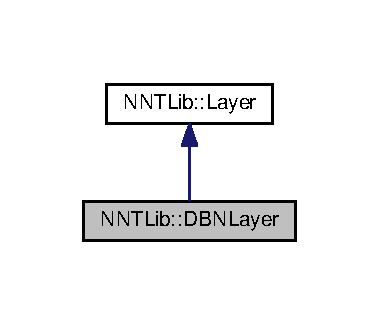
\includegraphics[width=182pt]{class_n_n_t_lib_1_1_d_b_n_layer__inherit__graph}
\end{center}
\end{figure}


Collaboration diagram for N\+N\+T\+Lib\+:\+:D\+B\+N\+Layer\+:\nopagebreak
\begin{figure}[H]
\begin{center}
\leavevmode
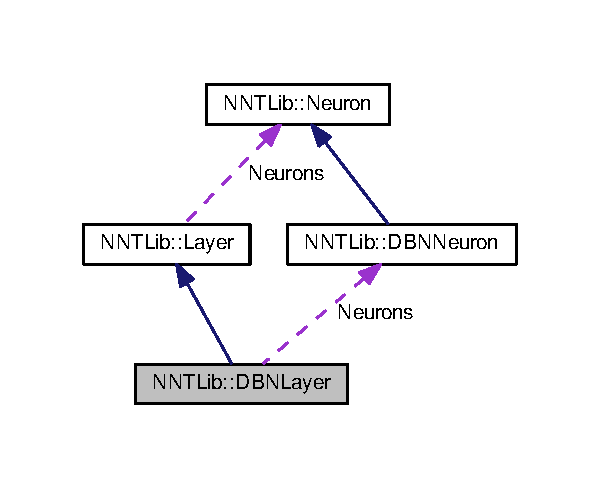
\includegraphics[width=288pt]{class_n_n_t_lib_1_1_d_b_n_layer__coll__graph}
\end{center}
\end{figure}
\subsection*{Public Member Functions}
\begin{DoxyCompactItemize}
\item 
void \hyperlink{class_n_n_t_lib_1_1_d_b_n_layer_ab6584bd72b2c0e095c8ddb58c1cc865d}{init} ()
\begin{DoxyCompactList}\small\item\em Initiliases \hyperlink{class_n_n_t_lib_1_1_layer}{Layer}. \end{DoxyCompactList}\item 
void \hyperlink{class_n_n_t_lib_1_1_d_b_n_layer_abde30250c496e42499d5bfcb79d6bcf9}{Init} (int inputsize, int neuron\+Count)
\begin{DoxyCompactList}\small\item\em Initialises \hyperlink{class_n_n_t_lib_1_1_layer}{Layer} with parameters. \end{DoxyCompactList}\item 
void \hyperlink{class_n_n_t_lib_1_1_d_b_n_layer_a3b0f2969d1fb6299f696ddb9ad1d198d}{Forwardweightsinit} (int inputsize, \hyperlink{class_n_n_t_lib_1_1_d_b_n_layer}{D\+B\+N\+Layer} $\ast$Layerup)
\begin{DoxyCompactList}\small\item\em Creates Forwardweights. \end{DoxyCompactList}\item 
\hyperlink{class_n_n_t_lib_1_1_d_b_n_layer_a1455fdf1fa76f4547bca76afee41e20f}{D\+B\+N\+Layer} ()
\begin{DoxyCompactList}\small\item\em Initializes a new instance of the \hyperlink{class_n_n_t_lib_1_1_d_b_n_layer}{D\+B\+N\+Layer} class. \end{DoxyCompactList}\item 
\hyperlink{class_n_n_t_lib_1_1_d_b_n_layer_ad7846b8b6b33704fe1ab27aa35d363a4}{$\sim$\+D\+B\+N\+Layer} ()
\begin{DoxyCompactList}\small\item\em Finalizes an instance of the \hyperlink{class_n_n_t_lib_1_1_d_b_n_layer}{D\+B\+N\+Layer} class. \end{DoxyCompactList}\item 
\hyperlink{class_n_n_t_lib_1_1_d_b_n_layer_a412a96132c7464a7502b203bc316920b}{D\+B\+N\+Layer} (const \hyperlink{class_n_n_t_lib_1_1_d_b_n_layer}{D\+B\+N\+Layer} \&that)
\begin{DoxyCompactList}\small\item\em copy constructor \end{DoxyCompactList}\item 
\hyperlink{class_n_n_t_lib_1_1_d_b_n_layer}{D\+B\+N\+Layer} \& \hyperlink{class_n_n_t_lib_1_1_d_b_n_layer_ac6c411ae0e17e002c89e93ebeefb6a11}{operator=} (const \hyperlink{class_n_n_t_lib_1_1_d_b_n_layer}{D\+B\+N\+Layer} \&that)
\begin{DoxyCompactList}\small\item\em overloaded = \end{DoxyCompactList}\end{DoxyCompactItemize}
\subsection*{Public Attributes}
\begin{DoxyCompactItemize}
\item 
\hyperlink{class_n_n_t_lib_1_1_d_b_n_neuron}{D\+B\+N\+Neuron} $\ast$ \hyperlink{class_n_n_t_lib_1_1_d_b_n_layer_ab499c1956d2198eaa0d64f6496be7557}{Neurons}
\end{DoxyCompactItemize}
\subsection*{Additional Inherited Members}


\subsection{Constructor \& Destructor Documentation}
\hypertarget{class_n_n_t_lib_1_1_d_b_n_layer_a1455fdf1fa76f4547bca76afee41e20f}{}\index{N\+N\+T\+Lib\+::\+D\+B\+N\+Layer@{N\+N\+T\+Lib\+::\+D\+B\+N\+Layer}!D\+B\+N\+Layer@{D\+B\+N\+Layer}}
\index{D\+B\+N\+Layer@{D\+B\+N\+Layer}!N\+N\+T\+Lib\+::\+D\+B\+N\+Layer@{N\+N\+T\+Lib\+::\+D\+B\+N\+Layer}}
\subsubsection[{D\+B\+N\+Layer}]{\setlength{\rightskip}{0pt plus 5cm}N\+N\+T\+Lib\+::\+D\+B\+N\+Layer\+::\+D\+B\+N\+Layer (
\begin{DoxyParamCaption}
{}
\end{DoxyParamCaption}
)}\label{class_n_n_t_lib_1_1_d_b_n_layer_a1455fdf1fa76f4547bca76afee41e20f}


Initializes a new instance of the \hyperlink{class_n_n_t_lib_1_1_d_b_n_layer}{D\+B\+N\+Layer} class. 

\hypertarget{class_n_n_t_lib_1_1_d_b_n_layer_ad7846b8b6b33704fe1ab27aa35d363a4}{}\index{N\+N\+T\+Lib\+::\+D\+B\+N\+Layer@{N\+N\+T\+Lib\+::\+D\+B\+N\+Layer}!````~D\+B\+N\+Layer@{$\sim$\+D\+B\+N\+Layer}}
\index{````~D\+B\+N\+Layer@{$\sim$\+D\+B\+N\+Layer}!N\+N\+T\+Lib\+::\+D\+B\+N\+Layer@{N\+N\+T\+Lib\+::\+D\+B\+N\+Layer}}
\subsubsection[{$\sim$\+D\+B\+N\+Layer}]{\setlength{\rightskip}{0pt plus 5cm}N\+N\+T\+Lib\+::\+D\+B\+N\+Layer\+::$\sim$\+D\+B\+N\+Layer (
\begin{DoxyParamCaption}
{}
\end{DoxyParamCaption}
)}\label{class_n_n_t_lib_1_1_d_b_n_layer_ad7846b8b6b33704fe1ab27aa35d363a4}


Finalizes an instance of the \hyperlink{class_n_n_t_lib_1_1_d_b_n_layer}{D\+B\+N\+Layer} class. 

\hypertarget{class_n_n_t_lib_1_1_d_b_n_layer_a412a96132c7464a7502b203bc316920b}{}\index{N\+N\+T\+Lib\+::\+D\+B\+N\+Layer@{N\+N\+T\+Lib\+::\+D\+B\+N\+Layer}!D\+B\+N\+Layer@{D\+B\+N\+Layer}}
\index{D\+B\+N\+Layer@{D\+B\+N\+Layer}!N\+N\+T\+Lib\+::\+D\+B\+N\+Layer@{N\+N\+T\+Lib\+::\+D\+B\+N\+Layer}}
\subsubsection[{D\+B\+N\+Layer}]{\setlength{\rightskip}{0pt plus 5cm}N\+N\+T\+Lib\+::\+D\+B\+N\+Layer\+::\+D\+B\+N\+Layer (
\begin{DoxyParamCaption}
\item[{const {\bf D\+B\+N\+Layer} \&}]{that}
\end{DoxyParamCaption}
)}\label{class_n_n_t_lib_1_1_d_b_n_layer_a412a96132c7464a7502b203bc316920b}


copy constructor 

copy constructor


\begin{DoxyParams}{Parameters}
{\em that} & \hyperlink{class_n_n_t_lib_1_1_layer}{Layer} to copy \\
\hline
\end{DoxyParams}


\subsection{Member Function Documentation}
\hypertarget{class_n_n_t_lib_1_1_d_b_n_layer_a3b0f2969d1fb6299f696ddb9ad1d198d}{}\index{N\+N\+T\+Lib\+::\+D\+B\+N\+Layer@{N\+N\+T\+Lib\+::\+D\+B\+N\+Layer}!Forwardweightsinit@{Forwardweightsinit}}
\index{Forwardweightsinit@{Forwardweightsinit}!N\+N\+T\+Lib\+::\+D\+B\+N\+Layer@{N\+N\+T\+Lib\+::\+D\+B\+N\+Layer}}
\subsubsection[{Forwardweightsinit}]{\setlength{\rightskip}{0pt plus 5cm}void N\+N\+T\+Lib\+::\+D\+B\+N\+Layer\+::\+Forwardweightsinit (
\begin{DoxyParamCaption}
\item[{int}]{Neuronsdown, }
\item[{{\bf D\+B\+N\+Layer} $\ast$}]{Layerup}
\end{DoxyParamCaption}
)}\label{class_n_n_t_lib_1_1_d_b_n_layer_a3b0f2969d1fb6299f696ddb9ad1d198d}


Creates Forwardweights. 

Sets Pointers to the weights from the layer above, making it easier to access them from the down \hyperlink{class_n_n_t_lib_1_1_layer}{Layer}


\begin{DoxyParams}{Parameters}
{\em Neuronsdown} & Number of Neurons on the down \hyperlink{class_n_n_t_lib_1_1_layer}{Layer} \\
\hline
{\em Layerup} & Pointer to the above \hyperlink{class_n_n_t_lib_1_1_layer}{Layer} \\
\hline
\end{DoxyParams}
\hypertarget{class_n_n_t_lib_1_1_d_b_n_layer_ab6584bd72b2c0e095c8ddb58c1cc865d}{}\index{N\+N\+T\+Lib\+::\+D\+B\+N\+Layer@{N\+N\+T\+Lib\+::\+D\+B\+N\+Layer}!init@{init}}
\index{init@{init}!N\+N\+T\+Lib\+::\+D\+B\+N\+Layer@{N\+N\+T\+Lib\+::\+D\+B\+N\+Layer}}
\subsubsection[{init}]{\setlength{\rightskip}{0pt plus 5cm}void N\+N\+T\+Lib\+::\+D\+B\+N\+Layer\+::init (
\begin{DoxyParamCaption}
{}
\end{DoxyParamCaption}
)}\label{class_n_n_t_lib_1_1_d_b_n_layer_ab6584bd72b2c0e095c8ddb58c1cc865d}


Initiliases \hyperlink{class_n_n_t_lib_1_1_layer}{Layer}. 

Simple Initialisation without parameters sets everything to 0 \hypertarget{class_n_n_t_lib_1_1_d_b_n_layer_abde30250c496e42499d5bfcb79d6bcf9}{}\index{N\+N\+T\+Lib\+::\+D\+B\+N\+Layer@{N\+N\+T\+Lib\+::\+D\+B\+N\+Layer}!Init@{Init}}
\index{Init@{Init}!N\+N\+T\+Lib\+::\+D\+B\+N\+Layer@{N\+N\+T\+Lib\+::\+D\+B\+N\+Layer}}
\subsubsection[{Init}]{\setlength{\rightskip}{0pt plus 5cm}void N\+N\+T\+Lib\+::\+D\+B\+N\+Layer\+::\+Init (
\begin{DoxyParamCaption}
\item[{int}]{inputsize, }
\item[{int}]{neuron\+Count}
\end{DoxyParamCaption}
)}\label{class_n_n_t_lib_1_1_d_b_n_layer_abde30250c496e42499d5bfcb79d6bcf9}


Initialises \hyperlink{class_n_n_t_lib_1_1_layer}{Layer} with parameters. 

Initialises the \hyperlink{class_n_n_t_lib_1_1_layer}{Layer} with Neurons, the number of inputvalues, the Deltas for errors in the weighst. Takes Care of building the weights Between Layers and that the Bias has no input weights


\begin{DoxyParams}{Parameters}
{\em inputsize} & Number of Inputs on the \hyperlink{class_n_n_t_lib_1_1_layer}{Layer} \\
\hline
{\em neuron\+Count} & Number of Neurons on the \hyperlink{class_n_n_t_lib_1_1_layer}{Layer} \\
\hline
\end{DoxyParams}
\hypertarget{class_n_n_t_lib_1_1_d_b_n_layer_ac6c411ae0e17e002c89e93ebeefb6a11}{}\index{N\+N\+T\+Lib\+::\+D\+B\+N\+Layer@{N\+N\+T\+Lib\+::\+D\+B\+N\+Layer}!operator=@{operator=}}
\index{operator=@{operator=}!N\+N\+T\+Lib\+::\+D\+B\+N\+Layer@{N\+N\+T\+Lib\+::\+D\+B\+N\+Layer}}
\subsubsection[{operator=}]{\setlength{\rightskip}{0pt plus 5cm}{\bf D\+B\+N\+Layer} \& N\+N\+T\+Lib\+::\+D\+B\+N\+Layer\+::operator= (
\begin{DoxyParamCaption}
\item[{const {\bf D\+B\+N\+Layer} \&}]{that}
\end{DoxyParamCaption}
)}\label{class_n_n_t_lib_1_1_d_b_n_layer_ac6c411ae0e17e002c89e93ebeefb6a11}


overloaded = 

Copies one layer into another


\begin{DoxyParams}{Parameters}
{\em that} & layer to copy \\
\hline
\end{DoxyParams}
\begin{DoxyReturn}{Returns}
new layer with copied values 
\end{DoxyReturn}


\subsection{Member Data Documentation}
\hypertarget{class_n_n_t_lib_1_1_d_b_n_layer_ab499c1956d2198eaa0d64f6496be7557}{}\index{N\+N\+T\+Lib\+::\+D\+B\+N\+Layer@{N\+N\+T\+Lib\+::\+D\+B\+N\+Layer}!Neurons@{Neurons}}
\index{Neurons@{Neurons}!N\+N\+T\+Lib\+::\+D\+B\+N\+Layer@{N\+N\+T\+Lib\+::\+D\+B\+N\+Layer}}
\subsubsection[{Neurons}]{\setlength{\rightskip}{0pt plus 5cm}{\bf D\+B\+N\+Neuron}$\ast$ N\+N\+T\+Lib\+::\+D\+B\+N\+Layer\+::\+Neurons}\label{class_n_n_t_lib_1_1_d_b_n_layer_ab499c1956d2198eaa0d64f6496be7557}
Deep Belief Neurons on the \hyperlink{class_n_n_t_lib_1_1_layer}{Layer} 

The documentation for this class was generated from the following files\+:\begin{DoxyCompactItemize}
\item 
N\+N\+T\+Lib/D\+B\+N\+Layer.\+h\item 
N\+N\+T\+Lib/D\+B\+N\+Layer.\+cpp\end{DoxyCompactItemize}

\hypertarget{class_n_n_t_lib_1_1_d_b_n_neuron}{}\section{N\+N\+T\+Lib\+:\+:D\+B\+N\+Neuron Class Reference}
\label{class_n_n_t_lib_1_1_d_b_n_neuron}\index{N\+N\+T\+Lib\+::\+D\+B\+N\+Neuron@{N\+N\+T\+Lib\+::\+D\+B\+N\+Neuron}}


Inheritance diagram for N\+N\+T\+Lib\+:\+:D\+B\+N\+Neuron\+:\nopagebreak
\begin{figure}[H]
\begin{center}
\leavevmode
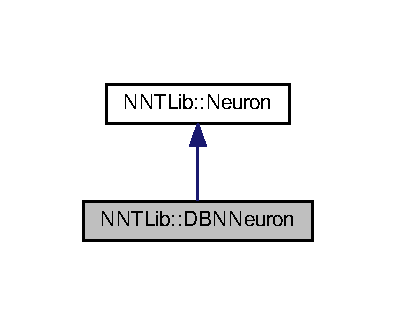
\includegraphics[width=190pt]{class_n_n_t_lib_1_1_d_b_n_neuron__inherit__graph}
\end{center}
\end{figure}


Collaboration diagram for N\+N\+T\+Lib\+:\+:D\+B\+N\+Neuron\+:\nopagebreak
\begin{figure}[H]
\begin{center}
\leavevmode
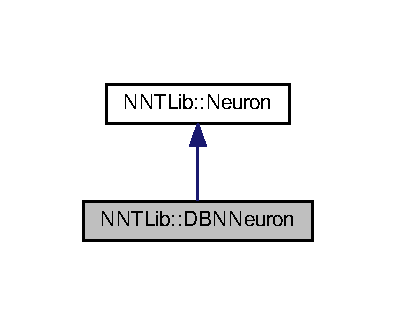
\includegraphics[width=190pt]{class_n_n_t_lib_1_1_d_b_n_neuron__coll__graph}
\end{center}
\end{figure}
\subsection*{Public Member Functions}
\begin{DoxyCompactItemize}
\item 
\hypertarget{class_n_n_t_lib_1_1_d_b_n_neuron_af445dc9c785101a92906545d17cfb332}{}\hyperlink{class_n_n_t_lib_1_1_d_b_n_neuron_af445dc9c785101a92906545d17cfb332}{D\+B\+N\+Neuron} ()\label{class_n_n_t_lib_1_1_d_b_n_neuron_af445dc9c785101a92906545d17cfb332}

\begin{DoxyCompactList}\small\item\em standard constructor \end{DoxyCompactList}\item 
\hypertarget{class_n_n_t_lib_1_1_d_b_n_neuron_a91f7afaf8367909137ab6105b0127ef1}{}\hyperlink{class_n_n_t_lib_1_1_d_b_n_neuron_a91f7afaf8367909137ab6105b0127ef1}{$\sim$\+D\+B\+N\+Neuron} ()\label{class_n_n_t_lib_1_1_d_b_n_neuron_a91f7afaf8367909137ab6105b0127ef1}

\begin{DoxyCompactList}\small\item\em destructor \end{DoxyCompactList}\item 
\hyperlink{class_n_n_t_lib_1_1_d_b_n_neuron_a6330de84d719d3aebbb9c4f9cf965406}{D\+B\+N\+Neuron} (const \hyperlink{class_n_n_t_lib_1_1_d_b_n_neuron}{D\+B\+N\+Neuron} \&that)
\begin{DoxyCompactList}\small\item\em Copy Constructor. \end{DoxyCompactList}\item 
\hyperlink{class_n_n_t_lib_1_1_d_b_n_neuron}{D\+B\+N\+Neuron} \& \hyperlink{class_n_n_t_lib_1_1_d_b_n_neuron_af497635d4a76b2d53ee1d1b5bc3cf826}{operator=} (const \hyperlink{class_n_n_t_lib_1_1_d_b_n_neuron}{D\+B\+N\+Neuron} \&that)
\begin{DoxyCompactList}\small\item\em Overloads =. \end{DoxyCompactList}\item 
void \hyperlink{class_n_n_t_lib_1_1_d_b_n_neuron_a69e9a06d177d18859aaba03913334c5d}{Init\+Bias} (const \hyperlink{class_n_n_t_lib_1_1_data_container}{Data\+Container} $\ast$container)
\begin{DoxyCompactList}\small\item\em Initialises Biasneuron. \end{DoxyCompactList}\item 
void \hyperlink{class_n_n_t_lib_1_1_d_b_n_neuron_a3958cfcba3cc6a9e371056739a282893}{Init} (int weight\+Count)
\begin{DoxyCompactList}\small\item\em Initialises \hyperlink{class_n_n_t_lib_1_1_neuron}{Neuron}. \end{DoxyCompactList}\end{DoxyCompactItemize}
\subsection*{Public Attributes}
\begin{DoxyCompactItemize}
\item 
\hypertarget{class_n_n_t_lib_1_1_d_b_n_neuron_a3ad1778b3739e6bf1f232583e01ab714}{}int \hyperlink{class_n_n_t_lib_1_1_d_b_n_neuron_a3ad1778b3739e6bf1f232583e01ab714}{Forward\+Weight\+Count}\label{class_n_n_t_lib_1_1_d_b_n_neuron_a3ad1778b3739e6bf1f232583e01ab714}

\begin{DoxyCompactList}\small\item\em Number of Forwardweights. \end{DoxyCompactList}\item 
\hypertarget{class_n_n_t_lib_1_1_d_b_n_neuron_a01d8094168eaba8e4b04cb3c934ef407}{}double \hyperlink{class_n_n_t_lib_1_1_d_b_n_neuron_a01d8094168eaba8e4b04cb3c934ef407}{p}\label{class_n_n_t_lib_1_1_d_b_n_neuron_a01d8094168eaba8e4b04cb3c934ef407}

\begin{DoxyCompactList}\small\item\em propability to turn on \end{DoxyCompactList}\item 
\hypertarget{class_n_n_t_lib_1_1_d_b_n_neuron_a728f1107afb0cad3e812c142c0c521e7}{}double $\ast$$\ast$ \hyperlink{class_n_n_t_lib_1_1_d_b_n_neuron_a728f1107afb0cad3e812c142c0c521e7}{Forward\+Weights}\label{class_n_n_t_lib_1_1_d_b_n_neuron_a728f1107afb0cad3e812c142c0c521e7}

\begin{DoxyCompactList}\small\item\em Pointer to weights in the layer above. \end{DoxyCompactList}\end{DoxyCompactItemize}
\subsection*{Protected Member Functions}
\begin{DoxyCompactItemize}
\item 
void \hyperlink{class_n_n_t_lib_1_1_d_b_n_neuron_a57cc105d60cb4f2bbb257e50cd61293d}{copy} (const \hyperlink{class_n_n_t_lib_1_1_d_b_n_neuron}{D\+B\+N\+Neuron} \&that)
\begin{DoxyCompactList}\small\item\em Copies \hyperlink{class_n_n_t_lib_1_1_neuron}{Neuron}. \end{DoxyCompactList}\item 
void \hyperlink{class_n_n_t_lib_1_1_d_b_n_neuron_ab0b791c2fea33976217c0428cd0ec08d}{init} ()
\begin{DoxyCompactList}\small\item\em Initialises \hyperlink{class_n_n_t_lib_1_1_neuron}{Neuron} with default Values. \end{DoxyCompactList}\item 
void \hyperlink{class_n_n_t_lib_1_1_d_b_n_neuron_aa92465b17737bd88c5b1f6d11d7dbf22}{free\+Mem} ()
\begin{DoxyCompactList}\small\item\em Frees memory. \end{DoxyCompactList}\end{DoxyCompactItemize}


\subsection{Constructor \& Destructor Documentation}
\hypertarget{class_n_n_t_lib_1_1_d_b_n_neuron_a6330de84d719d3aebbb9c4f9cf965406}{}\index{N\+N\+T\+Lib\+::\+D\+B\+N\+Neuron@{N\+N\+T\+Lib\+::\+D\+B\+N\+Neuron}!D\+B\+N\+Neuron@{D\+B\+N\+Neuron}}
\index{D\+B\+N\+Neuron@{D\+B\+N\+Neuron}!N\+N\+T\+Lib\+::\+D\+B\+N\+Neuron@{N\+N\+T\+Lib\+::\+D\+B\+N\+Neuron}}
\subsubsection[{D\+B\+N\+Neuron}]{\setlength{\rightskip}{0pt plus 5cm}N\+N\+T\+Lib\+::\+D\+B\+N\+Neuron\+::\+D\+B\+N\+Neuron (
\begin{DoxyParamCaption}
\item[{const {\bf D\+B\+N\+Neuron} \&}]{that}
\end{DoxyParamCaption}
)}\label{class_n_n_t_lib_1_1_d_b_n_neuron_a6330de84d719d3aebbb9c4f9cf965406}


Copy Constructor. 


\begin{DoxyParams}{Parameters}
{\em that} & \hyperlink{class_n_n_t_lib_1_1_neuron}{Neuron} to copy \\
\hline
\end{DoxyParams}


\subsection{Member Function Documentation}
\hypertarget{class_n_n_t_lib_1_1_d_b_n_neuron_a57cc105d60cb4f2bbb257e50cd61293d}{}\index{N\+N\+T\+Lib\+::\+D\+B\+N\+Neuron@{N\+N\+T\+Lib\+::\+D\+B\+N\+Neuron}!copy@{copy}}
\index{copy@{copy}!N\+N\+T\+Lib\+::\+D\+B\+N\+Neuron@{N\+N\+T\+Lib\+::\+D\+B\+N\+Neuron}}
\subsubsection[{copy}]{\setlength{\rightskip}{0pt plus 5cm}void N\+N\+T\+Lib\+::\+D\+B\+N\+Neuron\+::copy (
\begin{DoxyParamCaption}
\item[{const {\bf D\+B\+N\+Neuron} \&}]{that}
\end{DoxyParamCaption}
)\hspace{0.3cm}{\ttfamily [protected]}}\label{class_n_n_t_lib_1_1_d_b_n_neuron_a57cc105d60cb4f2bbb257e50cd61293d}


Copies \hyperlink{class_n_n_t_lib_1_1_neuron}{Neuron}. 

Copies \hyperlink{class_n_n_t_lib_1_1_neuron}{Neuron} into a new one


\begin{DoxyParams}{Parameters}
{\em that} & \hyperlink{class_n_n_t_lib_1_1_neuron}{Neuron} to copy \\
\hline
\end{DoxyParams}
\hypertarget{class_n_n_t_lib_1_1_d_b_n_neuron_aa92465b17737bd88c5b1f6d11d7dbf22}{}\index{N\+N\+T\+Lib\+::\+D\+B\+N\+Neuron@{N\+N\+T\+Lib\+::\+D\+B\+N\+Neuron}!free\+Mem@{free\+Mem}}
\index{free\+Mem@{free\+Mem}!N\+N\+T\+Lib\+::\+D\+B\+N\+Neuron@{N\+N\+T\+Lib\+::\+D\+B\+N\+Neuron}}
\subsubsection[{free\+Mem}]{\setlength{\rightskip}{0pt plus 5cm}void N\+N\+T\+Lib\+::\+D\+B\+N\+Neuron\+::free\+Mem (
\begin{DoxyParamCaption}
{}
\end{DoxyParamCaption}
)\hspace{0.3cm}{\ttfamily [protected]}}\label{class_n_n_t_lib_1_1_d_b_n_neuron_aa92465b17737bd88c5b1f6d11d7dbf22}


Frees memory. 

deletes Forwardweights \hypertarget{class_n_n_t_lib_1_1_d_b_n_neuron_ab0b791c2fea33976217c0428cd0ec08d}{}\index{N\+N\+T\+Lib\+::\+D\+B\+N\+Neuron@{N\+N\+T\+Lib\+::\+D\+B\+N\+Neuron}!init@{init}}
\index{init@{init}!N\+N\+T\+Lib\+::\+D\+B\+N\+Neuron@{N\+N\+T\+Lib\+::\+D\+B\+N\+Neuron}}
\subsubsection[{init}]{\setlength{\rightskip}{0pt plus 5cm}void N\+N\+T\+Lib\+::\+D\+B\+N\+Neuron\+::init (
\begin{DoxyParamCaption}
{}
\end{DoxyParamCaption}
)\hspace{0.3cm}{\ttfamily [protected]}}\label{class_n_n_t_lib_1_1_d_b_n_neuron_ab0b791c2fea33976217c0428cd0ec08d}


Initialises \hyperlink{class_n_n_t_lib_1_1_neuron}{Neuron} with default Values. 

Sets everything to 0 and the bias to 1 \hypertarget{class_n_n_t_lib_1_1_d_b_n_neuron_a3958cfcba3cc6a9e371056739a282893}{}\index{N\+N\+T\+Lib\+::\+D\+B\+N\+Neuron@{N\+N\+T\+Lib\+::\+D\+B\+N\+Neuron}!Init@{Init}}
\index{Init@{Init}!N\+N\+T\+Lib\+::\+D\+B\+N\+Neuron@{N\+N\+T\+Lib\+::\+D\+B\+N\+Neuron}}
\subsubsection[{Init}]{\setlength{\rightskip}{0pt plus 5cm}void N\+N\+T\+Lib\+::\+D\+B\+N\+Neuron\+::\+Init (
\begin{DoxyParamCaption}
\item[{int}]{weight\+Count}
\end{DoxyParamCaption}
)}\label{class_n_n_t_lib_1_1_d_b_n_neuron_a3958cfcba3cc6a9e371056739a282893}


Initialises \hyperlink{class_n_n_t_lib_1_1_neuron}{Neuron}. 

Allocates weights, deltaeights and lastdeltaweights with weightcount and sets weightcount


\begin{DoxyParams}{Parameters}
{\em weight\+Count} & Number of Backward weights on the neuron \\
\hline
\end{DoxyParams}
\hypertarget{class_n_n_t_lib_1_1_d_b_n_neuron_a69e9a06d177d18859aaba03913334c5d}{}\index{N\+N\+T\+Lib\+::\+D\+B\+N\+Neuron@{N\+N\+T\+Lib\+::\+D\+B\+N\+Neuron}!Init\+Bias@{Init\+Bias}}
\index{Init\+Bias@{Init\+Bias}!N\+N\+T\+Lib\+::\+D\+B\+N\+Neuron@{N\+N\+T\+Lib\+::\+D\+B\+N\+Neuron}}
\subsubsection[{Init\+Bias}]{\setlength{\rightskip}{0pt plus 5cm}void N\+N\+T\+Lib\+::\+D\+B\+N\+Neuron\+::\+Init\+Bias (
\begin{DoxyParamCaption}
\item[{const {\bf Data\+Container} $\ast$}]{container}
\end{DoxyParamCaption}
)}\label{class_n_n_t_lib_1_1_d_b_n_neuron_a69e9a06d177d18859aaba03913334c5d}


Initialises Biasneuron. 

Calculates \$\mbox{[}p\+\_\+i/(1-\/p\+\_\+i)\mbox{]}\$ with \$p\+\_\+i\$ as the average propability that a neuron turns on vor the visible layer. Hidden \hyperlink{class_n_n_t_lib_1_1_layer}{Layer} gets Bias set to 0.


\begin{DoxyParams}{Parameters}
{\em container} & Datacontainer with the probabilites for every training example \\
\hline
\end{DoxyParams}
\hypertarget{class_n_n_t_lib_1_1_d_b_n_neuron_af497635d4a76b2d53ee1d1b5bc3cf826}{}\index{N\+N\+T\+Lib\+::\+D\+B\+N\+Neuron@{N\+N\+T\+Lib\+::\+D\+B\+N\+Neuron}!operator=@{operator=}}
\index{operator=@{operator=}!N\+N\+T\+Lib\+::\+D\+B\+N\+Neuron@{N\+N\+T\+Lib\+::\+D\+B\+N\+Neuron}}
\subsubsection[{operator=}]{\setlength{\rightskip}{0pt plus 5cm}{\bf D\+B\+N\+Neuron} \& N\+N\+T\+Lib\+::\+D\+B\+N\+Neuron\+::operator= (
\begin{DoxyParamCaption}
\item[{const {\bf D\+B\+N\+Neuron} \&}]{that}
\end{DoxyParamCaption}
)}\label{class_n_n_t_lib_1_1_d_b_n_neuron_af497635d4a76b2d53ee1d1b5bc3cf826}


Overloads =. 


\begin{DoxyParams}{Parameters}
{\em that} & \hyperlink{class_n_n_t_lib_1_1_neuron}{Neuron} to copy \\
\hline
\end{DoxyParams}
\begin{DoxyReturn}{Returns}
new \hyperlink{class_n_n_t_lib_1_1_neuron}{Neuron} with copied values 
\end{DoxyReturn}


The documentation for this class was generated from the following files\+:\begin{DoxyCompactItemize}
\item 
N\+N\+T\+Lib/D\+B\+N\+Neuron.\+h\item 
N\+N\+T\+Lib/D\+B\+N\+Neuron.\+cpp\end{DoxyCompactItemize}

\hypertarget{class_n_n_t_lib_1_1_deep_belief_net}{}\section{N\+N\+T\+Lib\+:\+:Deep\+Belief\+Net Class Reference}
\label{class_n_n_t_lib_1_1_deep_belief_net}\index{N\+N\+T\+Lib\+::\+Deep\+Belief\+Net@{N\+N\+T\+Lib\+::\+Deep\+Belief\+Net}}


Inheritance diagram for N\+N\+T\+Lib\+:\+:Deep\+Belief\+Net\+:\nopagebreak
\begin{figure}[H]
\begin{center}
\leavevmode
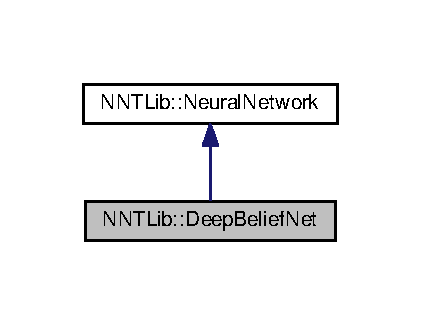
\includegraphics[width=202pt]{class_n_n_t_lib_1_1_deep_belief_net__inherit__graph}
\end{center}
\end{figure}


Collaboration diagram for N\+N\+T\+Lib\+:\+:Deep\+Belief\+Net\+:\nopagebreak
\begin{figure}[H]
\begin{center}
\leavevmode
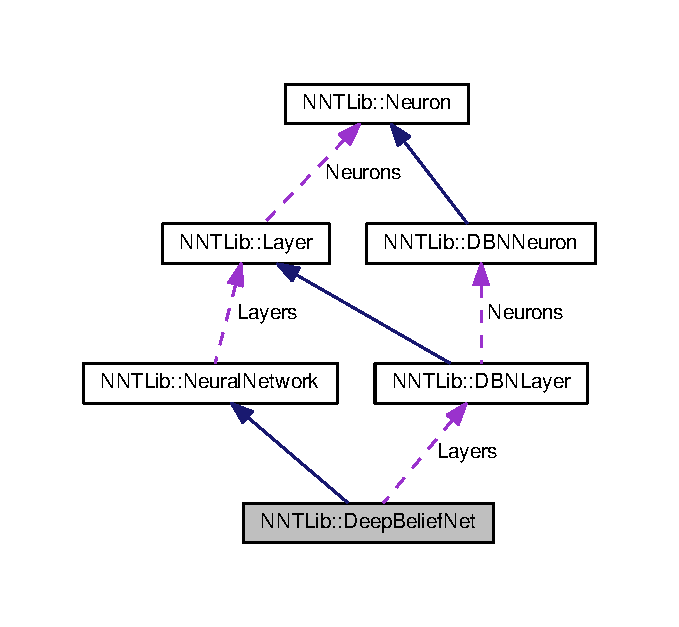
\includegraphics[width=326pt]{class_n_n_t_lib_1_1_deep_belief_net__coll__graph}
\end{center}
\end{figure}
\subsection*{Public Member Functions}
\begin{DoxyCompactItemize}
\item 
\hyperlink{class_n_n_t_lib_1_1_deep_belief_net_acaac4b567554fcbcfb2690d9cb2e1efb}{$\sim$\+Deep\+Belief\+Net} ()
\begin{DoxyCompactList}\small\item\em destructor \end{DoxyCompactList}\item 
\hyperlink{class_n_n_t_lib_1_1_deep_belief_net_a73dd53469742f45e085b2da799931b2c}{Deep\+Belief\+Net} (int $\ast$layers, int layercount, Weight\+Init\+Enum init\+Type, Function\+Enum function\+Type)
\begin{DoxyCompactList}\small\item\em Constructor. \end{DoxyCompactList}\item 
\hyperlink{class_n_n_t_lib_1_1_deep_belief_net_a4b15eba4fe97f8ef08478e3899fd72e6}{Deep\+Belief\+Net} (const \hyperlink{class_n_n_t_lib_1_1_deep_belief_net}{Deep\+Belief\+Net} \&that)
\begin{DoxyCompactList}\small\item\em Copy Constructor. \end{DoxyCompactList}\item 
void \hyperlink{class_n_n_t_lib_1_1_deep_belief_net_ab113a29355cce8baeb02db2f24b82396}{Init\+Weights} (Weight\+Init\+Enum init\+Type)
\begin{DoxyCompactList}\small\item\em Initialises Weights. \end{DoxyCompactList}\item 
void \hyperlink{class_n_n_t_lib_1_1_deep_belief_net_a665aa122bef611a89fd6aaaf818dbca1}{Save\+Weightsfor\+N\+N} (const std\+::string file)
\begin{DoxyCompactList}\small\item\em Saves Weights for neural network. \end{DoxyCompactList}\end{DoxyCompactItemize}
\subsection*{Public Attributes}
\begin{DoxyCompactItemize}
\item 
\hypertarget{class_n_n_t_lib_1_1_deep_belief_net_a21888da16f416fe46f75945b84d5ecba}{}\hyperlink{class_n_n_t_lib_1_1_d_b_n_layer}{D\+B\+N\+Layer} $\ast$ {\bfseries Layers}\label{class_n_n_t_lib_1_1_deep_belief_net_a21888da16f416fe46f75945b84d5ecba}

\end{DoxyCompactItemize}
\subsection*{Protected Member Functions}
\begin{DoxyCompactItemize}
\item 
void \hyperlink{class_n_n_t_lib_1_1_deep_belief_net_a19366c4ffaa837f4b4e2a73370d0e7b1}{copy} (const \hyperlink{class_n_n_t_lib_1_1_deep_belief_net}{Deep\+Belief\+Net} \&that)
\begin{DoxyCompactList}\small\item\em copies one Net into another \end{DoxyCompactList}\item 
void \hyperlink{class_n_n_t_lib_1_1_deep_belief_net_ad56044ef26b9980d3d577f9c71ba209e}{init} ()
\begin{DoxyCompactList}\small\item\em Initializes this instance. \end{DoxyCompactList}\item 
\hypertarget{class_n_n_t_lib_1_1_deep_belief_net_affb155c266325f3b7047cbc735bfd133}{}void {\bfseries free\+Mem} ()\label{class_n_n_t_lib_1_1_deep_belief_net_affb155c266325f3b7047cbc735bfd133}

\end{DoxyCompactItemize}
\subsection*{Protected Attributes}
\begin{DoxyCompactItemize}
\item 
\hypertarget{class_n_n_t_lib_1_1_deep_belief_net_ae6411b17e087b77332fe27b5d2a81458}{}std\+::mt19937 {\bfseries generator}\label{class_n_n_t_lib_1_1_deep_belief_net_ae6411b17e087b77332fe27b5d2a81458}

\end{DoxyCompactItemize}


\subsection{Constructor \& Destructor Documentation}
\hypertarget{class_n_n_t_lib_1_1_deep_belief_net_acaac4b567554fcbcfb2690d9cb2e1efb}{}\index{N\+N\+T\+Lib\+::\+Deep\+Belief\+Net@{N\+N\+T\+Lib\+::\+Deep\+Belief\+Net}!````~Deep\+Belief\+Net@{$\sim$\+Deep\+Belief\+Net}}
\index{````~Deep\+Belief\+Net@{$\sim$\+Deep\+Belief\+Net}!N\+N\+T\+Lib\+::\+Deep\+Belief\+Net@{N\+N\+T\+Lib\+::\+Deep\+Belief\+Net}}
\subsubsection[{$\sim$\+Deep\+Belief\+Net}]{\setlength{\rightskip}{0pt plus 5cm}N\+N\+T\+Lib\+::\+Deep\+Belief\+Net\+::$\sim$\+Deep\+Belief\+Net (
\begin{DoxyParamCaption}
{}
\end{DoxyParamCaption}
)}\label{class_n_n_t_lib_1_1_deep_belief_net_acaac4b567554fcbcfb2690d9cb2e1efb}


destructor 

destructor \hypertarget{class_n_n_t_lib_1_1_deep_belief_net_a73dd53469742f45e085b2da799931b2c}{}\index{N\+N\+T\+Lib\+::\+Deep\+Belief\+Net@{N\+N\+T\+Lib\+::\+Deep\+Belief\+Net}!Deep\+Belief\+Net@{Deep\+Belief\+Net}}
\index{Deep\+Belief\+Net@{Deep\+Belief\+Net}!N\+N\+T\+Lib\+::\+Deep\+Belief\+Net@{N\+N\+T\+Lib\+::\+Deep\+Belief\+Net}}
\subsubsection[{Deep\+Belief\+Net}]{\setlength{\rightskip}{0pt plus 5cm}N\+N\+T\+Lib\+::\+Deep\+Belief\+Net\+::\+Deep\+Belief\+Net (
\begin{DoxyParamCaption}
\item[{int $\ast$}]{neurons\+Count\+Per\+Layer, }
\item[{int}]{layercount, }
\item[{Weight\+Init\+Enum}]{init\+Type, }
\item[{Function\+Enum}]{function\+Type}
\end{DoxyParamCaption}
)}\label{class_n_n_t_lib_1_1_deep_belief_net_a73dd53469742f45e085b2da799931b2c}


Constructor. 

Initiliases the Deep Belief Net and builds it


\begin{DoxyParams}{Parameters}
{\em neurons\+Count\+Per\+Layer} & Array with the number of Neurons for every layer \\
\hline
{\em layercount} & Number of Layers \\
\hline
{\em init\+Type} & Which way to initialise Weights should be used \\
\hline
{\em function\+Type} & Which activation function is used in the neurons \\
\hline
\end{DoxyParams}
\hypertarget{class_n_n_t_lib_1_1_deep_belief_net_a4b15eba4fe97f8ef08478e3899fd72e6}{}\index{N\+N\+T\+Lib\+::\+Deep\+Belief\+Net@{N\+N\+T\+Lib\+::\+Deep\+Belief\+Net}!Deep\+Belief\+Net@{Deep\+Belief\+Net}}
\index{Deep\+Belief\+Net@{Deep\+Belief\+Net}!N\+N\+T\+Lib\+::\+Deep\+Belief\+Net@{N\+N\+T\+Lib\+::\+Deep\+Belief\+Net}}
\subsubsection[{Deep\+Belief\+Net}]{\setlength{\rightskip}{0pt plus 5cm}N\+N\+T\+Lib\+::\+Deep\+Belief\+Net\+::\+Deep\+Belief\+Net (
\begin{DoxyParamCaption}
\item[{const {\bf Deep\+Belief\+Net} \&}]{that}
\end{DoxyParamCaption}
)}\label{class_n_n_t_lib_1_1_deep_belief_net_a4b15eba4fe97f8ef08478e3899fd72e6}


Copy Constructor. 


\begin{DoxyParams}{Parameters}
{\em that} & Net to copy \\
\hline
\end{DoxyParams}


\subsection{Member Function Documentation}
\hypertarget{class_n_n_t_lib_1_1_deep_belief_net_a19366c4ffaa837f4b4e2a73370d0e7b1}{}\index{N\+N\+T\+Lib\+::\+Deep\+Belief\+Net@{N\+N\+T\+Lib\+::\+Deep\+Belief\+Net}!copy@{copy}}
\index{copy@{copy}!N\+N\+T\+Lib\+::\+Deep\+Belief\+Net@{N\+N\+T\+Lib\+::\+Deep\+Belief\+Net}}
\subsubsection[{copy}]{\setlength{\rightskip}{0pt plus 5cm}void N\+N\+T\+Lib\+::\+Deep\+Belief\+Net\+::copy (
\begin{DoxyParamCaption}
\item[{const {\bf Deep\+Belief\+Net} \&}]{that}
\end{DoxyParamCaption}
)\hspace{0.3cm}{\ttfamily [protected]}}\label{class_n_n_t_lib_1_1_deep_belief_net_a19366c4ffaa837f4b4e2a73370d0e7b1}


copies one Net into another 


\begin{DoxyParams}{Parameters}
{\em that} & Net to copy \\
\hline
\end{DoxyParams}
\hypertarget{class_n_n_t_lib_1_1_deep_belief_net_ad56044ef26b9980d3d577f9c71ba209e}{}\index{N\+N\+T\+Lib\+::\+Deep\+Belief\+Net@{N\+N\+T\+Lib\+::\+Deep\+Belief\+Net}!init@{init}}
\index{init@{init}!N\+N\+T\+Lib\+::\+Deep\+Belief\+Net@{N\+N\+T\+Lib\+::\+Deep\+Belief\+Net}}
\subsubsection[{init}]{\setlength{\rightskip}{0pt plus 5cm}void N\+N\+T\+Lib\+::\+Deep\+Belief\+Net\+::init (
\begin{DoxyParamCaption}
{}
\end{DoxyParamCaption}
)\hspace{0.3cm}{\ttfamily [protected]}}\label{class_n_n_t_lib_1_1_deep_belief_net_ad56044ef26b9980d3d577f9c71ba209e}


Initializes this instance. 

\hypertarget{class_n_n_t_lib_1_1_deep_belief_net_ab113a29355cce8baeb02db2f24b82396}{}\index{N\+N\+T\+Lib\+::\+Deep\+Belief\+Net@{N\+N\+T\+Lib\+::\+Deep\+Belief\+Net}!Init\+Weights@{Init\+Weights}}
\index{Init\+Weights@{Init\+Weights}!N\+N\+T\+Lib\+::\+Deep\+Belief\+Net@{N\+N\+T\+Lib\+::\+Deep\+Belief\+Net}}
\subsubsection[{Init\+Weights}]{\setlength{\rightskip}{0pt plus 5cm}void N\+N\+T\+Lib\+::\+Deep\+Belief\+Net\+::\+Init\+Weights (
\begin{DoxyParamCaption}
\item[{Weight\+Init\+Enum}]{init\+Type}
\end{DoxyParamCaption}
)}\label{class_n_n_t_lib_1_1_deep_belief_net_ab113a29355cce8baeb02db2f24b82396}


Initialises Weights. 

Initialises backward Weights for every \hyperlink{class_n_n_t_lib_1_1_neuron}{Neuron} in the net


\begin{DoxyParams}{Parameters}
{\em init\+Type} & Which type of intialisation should be used \\
\hline
\end{DoxyParams}
\hypertarget{class_n_n_t_lib_1_1_deep_belief_net_a665aa122bef611a89fd6aaaf818dbca1}{}\index{N\+N\+T\+Lib\+::\+Deep\+Belief\+Net@{N\+N\+T\+Lib\+::\+Deep\+Belief\+Net}!Save\+Weightsfor\+N\+N@{Save\+Weightsfor\+N\+N}}
\index{Save\+Weightsfor\+N\+N@{Save\+Weightsfor\+N\+N}!N\+N\+T\+Lib\+::\+Deep\+Belief\+Net@{N\+N\+T\+Lib\+::\+Deep\+Belief\+Net}}
\subsubsection[{Save\+Weightsfor\+N\+N}]{\setlength{\rightskip}{0pt plus 5cm}void N\+N\+T\+Lib\+::\+Deep\+Belief\+Net\+::\+Save\+Weightsfor\+N\+N (
\begin{DoxyParamCaption}
\item[{const std\+::string}]{file}
\end{DoxyParamCaption}
)}\label{class_n_n_t_lib_1_1_deep_belief_net_a665aa122bef611a89fd6aaaf818dbca1}


Saves Weights for neural network. 

Save weights in a way that a normal feedforward net can easily read them. The backward bias weights get lost in the process


\begin{DoxyParams}{Parameters}
{\em file} & Path to file that gets the weights \\
\hline
\end{DoxyParams}


The documentation for this class was generated from the following files\+:\begin{DoxyCompactItemize}
\item 
N\+N\+T\+Lib/Deep\+Belief\+Net.\+h\item 
N\+N\+T\+Lib/Deep\+Belief\+Net.\+cpp\end{DoxyCompactItemize}

\hypertarget{class_n_n_t_lib_1_1_genetic_algorithm}{}\section{N\+N\+T\+Lib\+:\+:Genetic\+Algorithm Class Reference}
\label{class_n_n_t_lib_1_1_genetic_algorithm}\index{N\+N\+T\+Lib\+::\+Genetic\+Algorithm@{N\+N\+T\+Lib\+::\+Genetic\+Algorithm}}


Inheritance diagram for N\+N\+T\+Lib\+:\+:Genetic\+Algorithm\+:\nopagebreak
\begin{figure}[H]
\begin{center}
\leavevmode
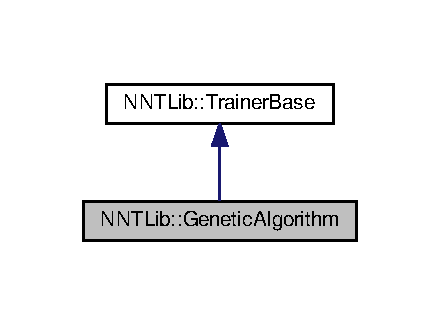
\includegraphics[width=211pt]{class_n_n_t_lib_1_1_genetic_algorithm__inherit__graph}
\end{center}
\end{figure}


Collaboration diagram for N\+N\+T\+Lib\+:\+:Genetic\+Algorithm\+:\nopagebreak
\begin{figure}[H]
\begin{center}
\leavevmode
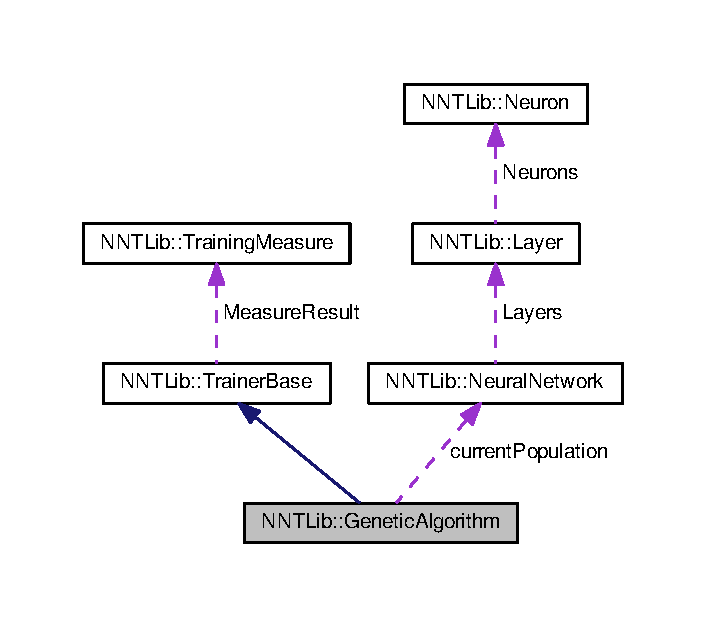
\includegraphics[width=339pt]{class_n_n_t_lib_1_1_genetic_algorithm__coll__graph}
\end{center}
\end{figure}
\subsection*{Public Member Functions}
\begin{DoxyCompactItemize}
\item 
\hyperlink{class_n_n_t_lib_1_1_genetic_algorithm_a19cd4345ff1f8950b830316fbabc95c5}{Genetic\+Algorithm} (\hyperlink{class_n_n_t_lib_1_1_neural_network}{Neural\+Network} $\ast$$\ast$\hyperlink{class_n_n_t_lib_1_1_genetic_algorithm_a0cc66a7ab5e6b5076a9abb701f194989}{current\+Population}, int populationsize)
\begin{DoxyCompactList}\small\item\em Initializes a new instance of the \hyperlink{class_n_n_t_lib_1_1_genetic_algorithm}{Genetic\+Algorithm} class. \end{DoxyCompactList}\item 
\hyperlink{class_n_n_t_lib_1_1_genetic_algorithm_aa2c7534da0fbf65548a372acc20f32e7}{$\sim$\+Genetic\+Algorithm} ()
\begin{DoxyCompactList}\small\item\em Finalizes an instance of the \hyperlink{class_n_n_t_lib_1_1_genetic_algorithm}{Genetic\+Algorithm} class. \end{DoxyCompactList}\item 
void \hyperlink{class_n_n_t_lib_1_1_genetic_algorithm_a98e2476f887049587d905917a898ad5c}{Train} (const \hyperlink{class_n_n_t_lib_1_1_data_container}{Data\+Container} \&data\+Container, int max\+Loop\+Count, double error\+Threshold, Mutate\+Enum mutate\+Type, Crossover\+Enum crossover\+Type, Roulette\+Enum roulette\+Type, int eltism\+Count, double mutation\+Probability=0.\+1, double crossover\+Probability=0.\+8, int mutate\+Node\+Count=0)
\begin{DoxyCompactList}\small\item\em Trains the specified data container. \end{DoxyCompactList}\end{DoxyCompactItemize}
\subsection*{Public Attributes}
\begin{DoxyCompactItemize}
\item 
\hyperlink{class_n_n_t_lib_1_1_neural_network}{Neural\+Network} $\ast$$\ast$ \hyperlink{class_n_n_t_lib_1_1_genetic_algorithm_a0cc66a7ab5e6b5076a9abb701f194989}{current\+Population}
\begin{DoxyCompactList}\small\item\em The current population \end{DoxyCompactList}\end{DoxyCompactItemize}
\subsection*{Additional Inherited Members}


\subsection{Constructor \& Destructor Documentation}
\hypertarget{class_n_n_t_lib_1_1_genetic_algorithm_a19cd4345ff1f8950b830316fbabc95c5}{}\index{N\+N\+T\+Lib\+::\+Genetic\+Algorithm@{N\+N\+T\+Lib\+::\+Genetic\+Algorithm}!Genetic\+Algorithm@{Genetic\+Algorithm}}
\index{Genetic\+Algorithm@{Genetic\+Algorithm}!N\+N\+T\+Lib\+::\+Genetic\+Algorithm@{N\+N\+T\+Lib\+::\+Genetic\+Algorithm}}
\subsubsection[{Genetic\+Algorithm}]{\setlength{\rightskip}{0pt plus 5cm}N\+N\+T\+Lib\+::\+Genetic\+Algorithm\+::\+Genetic\+Algorithm (
\begin{DoxyParamCaption}
\item[{{\bf Neural\+Network} $\ast$$\ast$}]{currentpopulation, }
\item[{int}]{populationsize}
\end{DoxyParamCaption}
)}\label{class_n_n_t_lib_1_1_genetic_algorithm_a19cd4345ff1f8950b830316fbabc95c5}


Initializes a new instance of the \hyperlink{class_n_n_t_lib_1_1_genetic_algorithm}{Genetic\+Algorithm} class. 


\begin{DoxyParams}{Parameters}
{\em current\+Population} & The current population.\\
\hline
{\em population\+Size} & Size of the population.\\
\hline
\end{DoxyParams}


Initializes a new instance of the \hyperlink{class_n_n_t_lib_1_1_genetic_algorithm}{Genetic\+Algorithm} class. 


\begin{DoxyParams}{Parameters}
{\em current\+Population} & The current population.\\
\hline
{\em populationsize} & The populationsize.\\
\hline
\end{DoxyParams}
\hypertarget{class_n_n_t_lib_1_1_genetic_algorithm_aa2c7534da0fbf65548a372acc20f32e7}{}\index{N\+N\+T\+Lib\+::\+Genetic\+Algorithm@{N\+N\+T\+Lib\+::\+Genetic\+Algorithm}!````~Genetic\+Algorithm@{$\sim$\+Genetic\+Algorithm}}
\index{````~Genetic\+Algorithm@{$\sim$\+Genetic\+Algorithm}!N\+N\+T\+Lib\+::\+Genetic\+Algorithm@{N\+N\+T\+Lib\+::\+Genetic\+Algorithm}}
\subsubsection[{$\sim$\+Genetic\+Algorithm}]{\setlength{\rightskip}{0pt plus 5cm}N\+N\+T\+Lib\+::\+Genetic\+Algorithm\+::$\sim$\+Genetic\+Algorithm (
\begin{DoxyParamCaption}
{}
\end{DoxyParamCaption}
)}\label{class_n_n_t_lib_1_1_genetic_algorithm_aa2c7534da0fbf65548a372acc20f32e7}


Finalizes an instance of the \hyperlink{class_n_n_t_lib_1_1_genetic_algorithm}{Genetic\+Algorithm} class. 



\subsection{Member Function Documentation}
\hypertarget{class_n_n_t_lib_1_1_genetic_algorithm_a98e2476f887049587d905917a898ad5c}{}\index{N\+N\+T\+Lib\+::\+Genetic\+Algorithm@{N\+N\+T\+Lib\+::\+Genetic\+Algorithm}!Train@{Train}}
\index{Train@{Train}!N\+N\+T\+Lib\+::\+Genetic\+Algorithm@{N\+N\+T\+Lib\+::\+Genetic\+Algorithm}}
\subsubsection[{Train}]{\setlength{\rightskip}{0pt plus 5cm}void N\+N\+T\+Lib\+::\+Genetic\+Algorithm\+::\+Train (
\begin{DoxyParamCaption}
\item[{const {\bf Data\+Container} \&}]{data\+Container, }
\item[{int}]{max\+Loop\+Count, }
\item[{double}]{error\+Threshold, }
\item[{Mutate\+Enum}]{mutate\+Type, }
\item[{Crossover\+Enum}]{crossover\+Type, }
\item[{Roulette\+Enum}]{roulette\+Type, }
\item[{int}]{eltism\+Count, }
\item[{double}]{mutation\+Probability = {\ttfamily 0.1}, }
\item[{double}]{crossover\+Probability = {\ttfamily 0.8}, }
\item[{int}]{mutate\+Node\+Count = {\ttfamily 0}}
\end{DoxyParamCaption}
)}\label{class_n_n_t_lib_1_1_genetic_algorithm_a98e2476f887049587d905917a898ad5c}


Trains the specified data container. 


\begin{DoxyParams}{Parameters}
{\em data\+Container} & The data container.\\
\hline
{\em max\+Loop\+Count} & The maximum loop count.\\
\hline
{\em error\+Threshold} & The error threshold.\\
\hline
{\em mutate\+Type} & Type of the mutate.\\
\hline
{\em crossover\+Type} & Type of the crossover.\\
\hline
{\em roulette\+Type} & Type of the roulette.\\
\hline
{\em eltism\+Count} & The eltism count.\\
\hline
{\em mutation\+Probability} & The mutation probability.\\
\hline
{\em crossover\+Probability} & The crossover probability.\\
\hline
{\em mutate\+Node\+Count} & The mutate node count.\\
\hline
\end{DoxyParams}


\subsection{Member Data Documentation}
\hypertarget{class_n_n_t_lib_1_1_genetic_algorithm_a0cc66a7ab5e6b5076a9abb701f194989}{}\index{N\+N\+T\+Lib\+::\+Genetic\+Algorithm@{N\+N\+T\+Lib\+::\+Genetic\+Algorithm}!current\+Population@{current\+Population}}
\index{current\+Population@{current\+Population}!N\+N\+T\+Lib\+::\+Genetic\+Algorithm@{N\+N\+T\+Lib\+::\+Genetic\+Algorithm}}
\subsubsection[{current\+Population}]{\setlength{\rightskip}{0pt plus 5cm}{\bf Neural\+Network}$\ast$$\ast$ N\+N\+T\+Lib\+::\+Genetic\+Algorithm\+::current\+Population}\label{class_n_n_t_lib_1_1_genetic_algorithm_a0cc66a7ab5e6b5076a9abb701f194989}


The current population 



The documentation for this class was generated from the following files\+:\begin{DoxyCompactItemize}
\item 
N\+N\+T\+Lib/Genetic\+Algorithm.\+h\item 
N\+N\+T\+Lib/Genetic\+Algorithm.\+cpp\end{DoxyCompactItemize}

\hypertarget{class_genetic_algorithm_config}{}\section{Genetic\+Algorithm\+Config Class Reference}
\label{class_genetic_algorithm_config}\index{Genetic\+Algorithm\+Config@{Genetic\+Algorithm\+Config}}


Inheritance diagram for Genetic\+Algorithm\+Config\+:\nopagebreak
\begin{figure}[H]
\begin{center}
\leavevmode
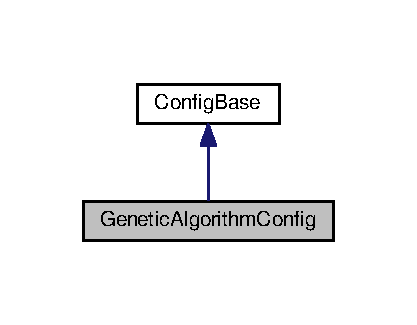
\includegraphics[width=200pt]{class_genetic_algorithm_config__inherit__graph}
\end{center}
\end{figure}


Collaboration diagram for Genetic\+Algorithm\+Config\+:\nopagebreak
\begin{figure}[H]
\begin{center}
\leavevmode
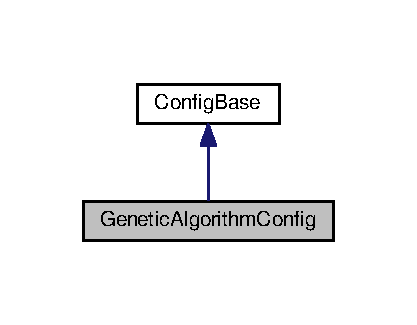
\includegraphics[width=200pt]{class_genetic_algorithm_config__coll__graph}
\end{center}
\end{figure}
\subsection*{Public Member Functions}
\begin{DoxyCompactItemize}
\item 
\hyperlink{class_genetic_algorithm_config_a1e36a3e666c730ec44dc232dbf3ee913}{Genetic\+Algorithm\+Config} ()
\begin{DoxyCompactList}\small\item\em Initializes a new instance of the \hyperlink{class_genetic_algorithm_config}{Genetic\+Algorithm\+Config} class. \end{DoxyCompactList}\item 
void \hyperlink{class_genetic_algorithm_config_ad77c035b3b7e5644834ef68aedfaef05}{Print\+Data} ()
\begin{DoxyCompactList}\small\item\em Prints the data. \end{DoxyCompactList}\item 
bool \hyperlink{class_genetic_algorithm_config_ae43b6c714d8d1e6f577dca4a5b9b068f}{Is\+Config\+Valid} ()
\begin{DoxyCompactList}\small\item\em Determines whether \mbox{[}is configuration valid\mbox{]}. \end{DoxyCompactList}\end{DoxyCompactItemize}
\subsection*{Public Attributes}
\begin{DoxyCompactItemize}
\item 
double \hyperlink{class_genetic_algorithm_config_ac4ebe8e0ea58e061871638a623ca016f}{Error\+Threshold}
\begin{DoxyCompactList}\small\item\em The error threshold \end{DoxyCompactList}\item 
int \hyperlink{class_genetic_algorithm_config_ae792cdb8d57ceef9a637ac3692e44fa9}{Max\+Loop\+Count}
\begin{DoxyCompactList}\small\item\em The maximum loop count \end{DoxyCompactList}\item 
N\+N\+T\+Lib\+::\+Mutate\+Enum \hyperlink{class_genetic_algorithm_config_ab6412ab79b082c2d36d241a03b8bea1a}{Mutate\+Type}
\begin{DoxyCompactList}\small\item\em The mutate type \end{DoxyCompactList}\item 
N\+N\+T\+Lib\+::\+Crossover\+Enum \hyperlink{class_genetic_algorithm_config_a3a812549ca573f20d6cafc3b651089ba}{Cross\+Type}
\begin{DoxyCompactList}\small\item\em The cross type \end{DoxyCompactList}\item 
N\+N\+T\+Lib\+::\+Roulette\+Enum \hyperlink{class_genetic_algorithm_config_abe0badd59b500a67a8179ca83bd7fea9}{Roulette\+Type}
\begin{DoxyCompactList}\small\item\em The roulette type \end{DoxyCompactList}\item 
int \hyperlink{class_genetic_algorithm_config_a8e8f286ff257bb31ab7c4a64963be30b}{Population\+Size}
\begin{DoxyCompactList}\small\item\em The population size \end{DoxyCompactList}\item 
int \hyperlink{class_genetic_algorithm_config_a410b565ccd042a3eb5bcf914b7eba1c4}{Eltism\+Count}
\begin{DoxyCompactList}\small\item\em The eltism count \end{DoxyCompactList}\item 
double \hyperlink{class_genetic_algorithm_config_ac9ecafde07cb2dee58d5dc0bb4d2afa9}{Mutation\+Probability}
\begin{DoxyCompactList}\small\item\em The mutation probability \end{DoxyCompactList}\item 
double \hyperlink{class_genetic_algorithm_config_aa20b937acb8421fd94deec043389708b}{Crossover\+Probability}
\begin{DoxyCompactList}\small\item\em The crossover probability \end{DoxyCompactList}\item 
int \hyperlink{class_genetic_algorithm_config_a79b354373f83b53c1acae61e3f6d7935}{Mutate\+Node\+Count}
\begin{DoxyCompactList}\small\item\em The mutate node count \end{DoxyCompactList}\end{DoxyCompactItemize}
\subsection*{Protected Member Functions}
\begin{DoxyCompactItemize}
\item 
void \hyperlink{class_genetic_algorithm_config_aa18ae6c8e8767ed64deb56748e6aa875}{Handle\+Name\+Value} (std\+::string name, std\+::string value)
\begin{DoxyCompactList}\small\item\em Handles the name value. \end{DoxyCompactList}\end{DoxyCompactItemize}


\subsection{Constructor \& Destructor Documentation}
\hypertarget{class_genetic_algorithm_config_a1e36a3e666c730ec44dc232dbf3ee913}{}\index{Genetic\+Algorithm\+Config@{Genetic\+Algorithm\+Config}!Genetic\+Algorithm\+Config@{Genetic\+Algorithm\+Config}}
\index{Genetic\+Algorithm\+Config@{Genetic\+Algorithm\+Config}!Genetic\+Algorithm\+Config@{Genetic\+Algorithm\+Config}}
\subsubsection[{Genetic\+Algorithm\+Config}]{\setlength{\rightskip}{0pt plus 5cm}Genetic\+Algorithm\+Config\+::\+Genetic\+Algorithm\+Config (
\begin{DoxyParamCaption}
{}
\end{DoxyParamCaption}
)}\label{class_genetic_algorithm_config_a1e36a3e666c730ec44dc232dbf3ee913}


Initializes a new instance of the \hyperlink{class_genetic_algorithm_config}{Genetic\+Algorithm\+Config} class. 



\subsection{Member Function Documentation}
\hypertarget{class_genetic_algorithm_config_aa18ae6c8e8767ed64deb56748e6aa875}{}\index{Genetic\+Algorithm\+Config@{Genetic\+Algorithm\+Config}!Handle\+Name\+Value@{Handle\+Name\+Value}}
\index{Handle\+Name\+Value@{Handle\+Name\+Value}!Genetic\+Algorithm\+Config@{Genetic\+Algorithm\+Config}}
\subsubsection[{Handle\+Name\+Value}]{\setlength{\rightskip}{0pt plus 5cm}void Genetic\+Algorithm\+Config\+::\+Handle\+Name\+Value (
\begin{DoxyParamCaption}
\item[{std\+::string}]{name, }
\item[{std\+::string}]{value}
\end{DoxyParamCaption}
)\hspace{0.3cm}{\ttfamily [protected]}, {\ttfamily [virtual]}}\label{class_genetic_algorithm_config_aa18ae6c8e8767ed64deb56748e6aa875}


Handles the name value. 


\begin{DoxyParams}{Parameters}
{\em name} & The name.\\
\hline
{\em value} & The value.\\
\hline
\end{DoxyParams}


Implements \hyperlink{class_config_base}{Config\+Base}.

\hypertarget{class_genetic_algorithm_config_ae43b6c714d8d1e6f577dca4a5b9b068f}{}\index{Genetic\+Algorithm\+Config@{Genetic\+Algorithm\+Config}!Is\+Config\+Valid@{Is\+Config\+Valid}}
\index{Is\+Config\+Valid@{Is\+Config\+Valid}!Genetic\+Algorithm\+Config@{Genetic\+Algorithm\+Config}}
\subsubsection[{Is\+Config\+Valid}]{\setlength{\rightskip}{0pt plus 5cm}bool Genetic\+Algorithm\+Config\+::\+Is\+Config\+Valid (
\begin{DoxyParamCaption}
{}
\end{DoxyParamCaption}
)\hspace{0.3cm}{\ttfamily [virtual]}}\label{class_genetic_algorithm_config_ae43b6c714d8d1e6f577dca4a5b9b068f}


Determines whether \mbox{[}is configuration valid\mbox{]}. 

\begin{DoxyReturn}{Returns}

\end{DoxyReturn}


Implements \hyperlink{class_config_base}{Config\+Base}.

\hypertarget{class_genetic_algorithm_config_ad77c035b3b7e5644834ef68aedfaef05}{}\index{Genetic\+Algorithm\+Config@{Genetic\+Algorithm\+Config}!Print\+Data@{Print\+Data}}
\index{Print\+Data@{Print\+Data}!Genetic\+Algorithm\+Config@{Genetic\+Algorithm\+Config}}
\subsubsection[{Print\+Data}]{\setlength{\rightskip}{0pt plus 5cm}void Genetic\+Algorithm\+Config\+::\+Print\+Data (
\begin{DoxyParamCaption}
{}
\end{DoxyParamCaption}
)\hspace{0.3cm}{\ttfamily [virtual]}}\label{class_genetic_algorithm_config_ad77c035b3b7e5644834ef68aedfaef05}


Prints the data. 



Implements \hyperlink{class_config_base}{Config\+Base}.



\subsection{Member Data Documentation}
\hypertarget{class_genetic_algorithm_config_aa20b937acb8421fd94deec043389708b}{}\index{Genetic\+Algorithm\+Config@{Genetic\+Algorithm\+Config}!Crossover\+Probability@{Crossover\+Probability}}
\index{Crossover\+Probability@{Crossover\+Probability}!Genetic\+Algorithm\+Config@{Genetic\+Algorithm\+Config}}
\subsubsection[{Crossover\+Probability}]{\setlength{\rightskip}{0pt plus 5cm}double Genetic\+Algorithm\+Config\+::\+Crossover\+Probability}\label{class_genetic_algorithm_config_aa20b937acb8421fd94deec043389708b}


The crossover probability 

\hypertarget{class_genetic_algorithm_config_a3a812549ca573f20d6cafc3b651089ba}{}\index{Genetic\+Algorithm\+Config@{Genetic\+Algorithm\+Config}!Cross\+Type@{Cross\+Type}}
\index{Cross\+Type@{Cross\+Type}!Genetic\+Algorithm\+Config@{Genetic\+Algorithm\+Config}}
\subsubsection[{Cross\+Type}]{\setlength{\rightskip}{0pt plus 5cm}N\+N\+T\+Lib\+::\+Crossover\+Enum Genetic\+Algorithm\+Config\+::\+Cross\+Type}\label{class_genetic_algorithm_config_a3a812549ca573f20d6cafc3b651089ba}


The cross type 

\hypertarget{class_genetic_algorithm_config_a410b565ccd042a3eb5bcf914b7eba1c4}{}\index{Genetic\+Algorithm\+Config@{Genetic\+Algorithm\+Config}!Eltism\+Count@{Eltism\+Count}}
\index{Eltism\+Count@{Eltism\+Count}!Genetic\+Algorithm\+Config@{Genetic\+Algorithm\+Config}}
\subsubsection[{Eltism\+Count}]{\setlength{\rightskip}{0pt plus 5cm}int Genetic\+Algorithm\+Config\+::\+Eltism\+Count}\label{class_genetic_algorithm_config_a410b565ccd042a3eb5bcf914b7eba1c4}


The eltism count 

\hypertarget{class_genetic_algorithm_config_ac4ebe8e0ea58e061871638a623ca016f}{}\index{Genetic\+Algorithm\+Config@{Genetic\+Algorithm\+Config}!Error\+Threshold@{Error\+Threshold}}
\index{Error\+Threshold@{Error\+Threshold}!Genetic\+Algorithm\+Config@{Genetic\+Algorithm\+Config}}
\subsubsection[{Error\+Threshold}]{\setlength{\rightskip}{0pt plus 5cm}double Genetic\+Algorithm\+Config\+::\+Error\+Threshold}\label{class_genetic_algorithm_config_ac4ebe8e0ea58e061871638a623ca016f}


The error threshold 

\hypertarget{class_genetic_algorithm_config_ae792cdb8d57ceef9a637ac3692e44fa9}{}\index{Genetic\+Algorithm\+Config@{Genetic\+Algorithm\+Config}!Max\+Loop\+Count@{Max\+Loop\+Count}}
\index{Max\+Loop\+Count@{Max\+Loop\+Count}!Genetic\+Algorithm\+Config@{Genetic\+Algorithm\+Config}}
\subsubsection[{Max\+Loop\+Count}]{\setlength{\rightskip}{0pt plus 5cm}int Genetic\+Algorithm\+Config\+::\+Max\+Loop\+Count}\label{class_genetic_algorithm_config_ae792cdb8d57ceef9a637ac3692e44fa9}


The maximum loop count 

\hypertarget{class_genetic_algorithm_config_a79b354373f83b53c1acae61e3f6d7935}{}\index{Genetic\+Algorithm\+Config@{Genetic\+Algorithm\+Config}!Mutate\+Node\+Count@{Mutate\+Node\+Count}}
\index{Mutate\+Node\+Count@{Mutate\+Node\+Count}!Genetic\+Algorithm\+Config@{Genetic\+Algorithm\+Config}}
\subsubsection[{Mutate\+Node\+Count}]{\setlength{\rightskip}{0pt plus 5cm}int Genetic\+Algorithm\+Config\+::\+Mutate\+Node\+Count}\label{class_genetic_algorithm_config_a79b354373f83b53c1acae61e3f6d7935}


The mutate node count 

\hypertarget{class_genetic_algorithm_config_ab6412ab79b082c2d36d241a03b8bea1a}{}\index{Genetic\+Algorithm\+Config@{Genetic\+Algorithm\+Config}!Mutate\+Type@{Mutate\+Type}}
\index{Mutate\+Type@{Mutate\+Type}!Genetic\+Algorithm\+Config@{Genetic\+Algorithm\+Config}}
\subsubsection[{Mutate\+Type}]{\setlength{\rightskip}{0pt plus 5cm}N\+N\+T\+Lib\+::\+Mutate\+Enum Genetic\+Algorithm\+Config\+::\+Mutate\+Type}\label{class_genetic_algorithm_config_ab6412ab79b082c2d36d241a03b8bea1a}


The mutate type 

\hypertarget{class_genetic_algorithm_config_ac9ecafde07cb2dee58d5dc0bb4d2afa9}{}\index{Genetic\+Algorithm\+Config@{Genetic\+Algorithm\+Config}!Mutation\+Probability@{Mutation\+Probability}}
\index{Mutation\+Probability@{Mutation\+Probability}!Genetic\+Algorithm\+Config@{Genetic\+Algorithm\+Config}}
\subsubsection[{Mutation\+Probability}]{\setlength{\rightskip}{0pt plus 5cm}double Genetic\+Algorithm\+Config\+::\+Mutation\+Probability}\label{class_genetic_algorithm_config_ac9ecafde07cb2dee58d5dc0bb4d2afa9}


The mutation probability 

\hypertarget{class_genetic_algorithm_config_a8e8f286ff257bb31ab7c4a64963be30b}{}\index{Genetic\+Algorithm\+Config@{Genetic\+Algorithm\+Config}!Population\+Size@{Population\+Size}}
\index{Population\+Size@{Population\+Size}!Genetic\+Algorithm\+Config@{Genetic\+Algorithm\+Config}}
\subsubsection[{Population\+Size}]{\setlength{\rightskip}{0pt plus 5cm}int Genetic\+Algorithm\+Config\+::\+Population\+Size}\label{class_genetic_algorithm_config_a8e8f286ff257bb31ab7c4a64963be30b}


The population size 

\hypertarget{class_genetic_algorithm_config_abe0badd59b500a67a8179ca83bd7fea9}{}\index{Genetic\+Algorithm\+Config@{Genetic\+Algorithm\+Config}!Roulette\+Type@{Roulette\+Type}}
\index{Roulette\+Type@{Roulette\+Type}!Genetic\+Algorithm\+Config@{Genetic\+Algorithm\+Config}}
\subsubsection[{Roulette\+Type}]{\setlength{\rightskip}{0pt plus 5cm}N\+N\+T\+Lib\+::\+Roulette\+Enum Genetic\+Algorithm\+Config\+::\+Roulette\+Type}\label{class_genetic_algorithm_config_abe0badd59b500a67a8179ca83bd7fea9}


The roulette type 



The documentation for this class was generated from the following files\+:\begin{DoxyCompactItemize}
\item 
N\+N\+T\+Lib/Genetic\+Algorithm\+Config.\+h\item 
N\+N\+T\+Lib/Genetic\+Algorithm\+Config.\+cpp\end{DoxyCompactItemize}

\hypertarget{class_n_n_t_lib_1_1_layer}{}\section{N\+N\+T\+Lib\+:\+:Layer Class Reference}
\label{class_n_n_t_lib_1_1_layer}\index{N\+N\+T\+Lib\+::\+Layer@{N\+N\+T\+Lib\+::\+Layer}}


Inheritance diagram for N\+N\+T\+Lib\+:\+:Layer\+:\nopagebreak
\begin{figure}[H]
\begin{center}
\leavevmode
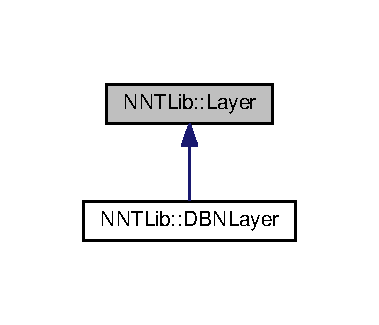
\includegraphics[width=182pt]{class_n_n_t_lib_1_1_layer__inherit__graph}
\end{center}
\end{figure}


Collaboration diagram for N\+N\+T\+Lib\+:\+:Layer\+:\nopagebreak
\begin{figure}[H]
\begin{center}
\leavevmode
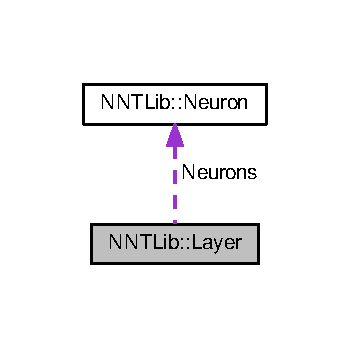
\includegraphics[width=168pt]{class_n_n_t_lib_1_1_layer__coll__graph}
\end{center}
\end{figure}
\subsection*{Public Member Functions}
\begin{DoxyCompactItemize}
\item 
void \hyperlink{class_n_n_t_lib_1_1_layer_acb8971ed21ec40118ba384750a0f5af8}{Init} (int inputsize, int neuron\+Count)
\begin{DoxyCompactList}\small\item\em Initializes the specified inputsize. \end{DoxyCompactList}\item 
\hyperlink{class_n_n_t_lib_1_1_layer_a4e30f7c8ff5426765c7c5b8f12c35c14}{Layer} ()
\begin{DoxyCompactList}\small\item\em Initializes a new instance of the \hyperlink{class_n_n_t_lib_1_1_layer}{Layer} class. \end{DoxyCompactList}\item 
\hyperlink{class_n_n_t_lib_1_1_layer_acd060e0c112f0ced1ce1530fa3e7e4bf}{$\sim$\+Layer} ()
\begin{DoxyCompactList}\small\item\em Finalizes an instance of the \hyperlink{class_n_n_t_lib_1_1_layer}{Layer} class. \end{DoxyCompactList}\item 
\hyperlink{class_n_n_t_lib_1_1_layer_acba87c68aaa9a258185bfe3a807cb841}{Layer} (const \hyperlink{class_n_n_t_lib_1_1_layer}{Layer} \&that)
\begin{DoxyCompactList}\small\item\em Initializes a new instance of the \hyperlink{class_n_n_t_lib_1_1_layer}{Layer} class. \end{DoxyCompactList}\item 
\hyperlink{class_n_n_t_lib_1_1_layer}{Layer} \& \hyperlink{class_n_n_t_lib_1_1_layer_aa7d4a78bec6093926dcf48eec2f87aeb}{operator=} (const \hyperlink{class_n_n_t_lib_1_1_layer}{Layer} \&that)
\begin{DoxyCompactList}\small\item\em Operator=s the specified that. \end{DoxyCompactList}\end{DoxyCompactItemize}
\subsection*{Public Attributes}
\begin{DoxyCompactItemize}
\item 
int \hyperlink{class_n_n_t_lib_1_1_layer_a5c968ed46039cbaa69f217c71fd74855}{Input\+Values\+Count}
\begin{DoxyCompactList}\small\item\em The input values count \end{DoxyCompactList}\item 
int \hyperlink{class_n_n_t_lib_1_1_layer_a3537c5d904445f7bebac1136c59e0503}{Input\+Values\+Count\+With\+Bias}
\begin{DoxyCompactList}\small\item\em The input values count with bias \end{DoxyCompactList}\item 
int \hyperlink{class_n_n_t_lib_1_1_layer_aba659d85237baa7e0b3ba235d5313da6}{Neuron\+Count}
\begin{DoxyCompactList}\small\item\em The neuron count \end{DoxyCompactList}\item 
\hyperlink{class_n_n_t_lib_1_1_neuron}{Neuron} $\ast$ \hyperlink{class_n_n_t_lib_1_1_layer_ae10597dc8e12d338fe40d902d6f26ef0}{Neurons}
\begin{DoxyCompactList}\small\item\em The neurons (Collection aller Neuronen auf dem \hyperlink{class_n_n_t_lib_1_1_layer}{Layer}) \end{DoxyCompactList}\item 
double $\ast$ \hyperlink{class_n_n_t_lib_1_1_layer_ab269c8597fa1768562515f8b68439b73}{Input\+Values}
\begin{DoxyCompactList}\small\item\em The input values (Collection mit Ausgaben des darunter liegenden Layers Li-\/1) \end{DoxyCompactList}\item 
double $\ast$ \hyperlink{class_n_n_t_lib_1_1_layer_a655484beac27344f2ced3bc77a9f160f}{Sum\+Delta\+Err\+Weights}
\begin{DoxyCompactList}\small\item\em The sum (delta $\ast$ error $\ast$ weights) \end{DoxyCompactList}\end{DoxyCompactItemize}
\subsection*{Protected Member Functions}
\begin{DoxyCompactItemize}
\item 
void \hyperlink{class_n_n_t_lib_1_1_layer_a1df43626aced41e9f4939c044acd7fdc}{copy} (const \hyperlink{class_n_n_t_lib_1_1_layer}{Layer} \&that)
\begin{DoxyCompactList}\small\item\em Copies the specified that. \end{DoxyCompactList}\item 
void \hyperlink{class_n_n_t_lib_1_1_layer_a77aaaad4b04400691070dd0172197f90}{init} ()
\begin{DoxyCompactList}\small\item\em Initializes this instance. \end{DoxyCompactList}\item 
void \hyperlink{class_n_n_t_lib_1_1_layer_a72cae10c49660e2c7e0788849fdf94df}{free\+Mem} ()
\begin{DoxyCompactList}\small\item\em Frees the memory. \end{DoxyCompactList}\end{DoxyCompactItemize}


\subsection{Constructor \& Destructor Documentation}
\hypertarget{class_n_n_t_lib_1_1_layer_a4e30f7c8ff5426765c7c5b8f12c35c14}{}\index{N\+N\+T\+Lib\+::\+Layer@{N\+N\+T\+Lib\+::\+Layer}!Layer@{Layer}}
\index{Layer@{Layer}!N\+N\+T\+Lib\+::\+Layer@{N\+N\+T\+Lib\+::\+Layer}}
\subsubsection[{Layer}]{\setlength{\rightskip}{0pt plus 5cm}N\+N\+T\+Lib\+::\+Layer\+::\+Layer (
\begin{DoxyParamCaption}
{}
\end{DoxyParamCaption}
)}\label{class_n_n_t_lib_1_1_layer_a4e30f7c8ff5426765c7c5b8f12c35c14}


Initializes a new instance of the \hyperlink{class_n_n_t_lib_1_1_layer}{Layer} class. 

\hypertarget{class_n_n_t_lib_1_1_layer_acd060e0c112f0ced1ce1530fa3e7e4bf}{}\index{N\+N\+T\+Lib\+::\+Layer@{N\+N\+T\+Lib\+::\+Layer}!````~Layer@{$\sim$\+Layer}}
\index{````~Layer@{$\sim$\+Layer}!N\+N\+T\+Lib\+::\+Layer@{N\+N\+T\+Lib\+::\+Layer}}
\subsubsection[{$\sim$\+Layer}]{\setlength{\rightskip}{0pt plus 5cm}N\+N\+T\+Lib\+::\+Layer\+::$\sim$\+Layer (
\begin{DoxyParamCaption}
{}
\end{DoxyParamCaption}
)}\label{class_n_n_t_lib_1_1_layer_acd060e0c112f0ced1ce1530fa3e7e4bf}


Finalizes an instance of the \hyperlink{class_n_n_t_lib_1_1_layer}{Layer} class. 

\hypertarget{class_n_n_t_lib_1_1_layer_acba87c68aaa9a258185bfe3a807cb841}{}\index{N\+N\+T\+Lib\+::\+Layer@{N\+N\+T\+Lib\+::\+Layer}!Layer@{Layer}}
\index{Layer@{Layer}!N\+N\+T\+Lib\+::\+Layer@{N\+N\+T\+Lib\+::\+Layer}}
\subsubsection[{Layer}]{\setlength{\rightskip}{0pt plus 5cm}N\+N\+T\+Lib\+::\+Layer\+::\+Layer (
\begin{DoxyParamCaption}
\item[{const {\bf Layer} \&}]{that}
\end{DoxyParamCaption}
)}\label{class_n_n_t_lib_1_1_layer_acba87c68aaa9a258185bfe3a807cb841}


Initializes a new instance of the \hyperlink{class_n_n_t_lib_1_1_layer}{Layer} class. 


\begin{DoxyParams}{Parameters}
{\em that} & The that.\\
\hline
\end{DoxyParams}


\subsection{Member Function Documentation}
\hypertarget{class_n_n_t_lib_1_1_layer_a1df43626aced41e9f4939c044acd7fdc}{}\index{N\+N\+T\+Lib\+::\+Layer@{N\+N\+T\+Lib\+::\+Layer}!copy@{copy}}
\index{copy@{copy}!N\+N\+T\+Lib\+::\+Layer@{N\+N\+T\+Lib\+::\+Layer}}
\subsubsection[{copy}]{\setlength{\rightskip}{0pt plus 5cm}void N\+N\+T\+Lib\+::\+Layer\+::copy (
\begin{DoxyParamCaption}
\item[{const {\bf Layer} \&}]{that}
\end{DoxyParamCaption}
)\hspace{0.3cm}{\ttfamily [protected]}}\label{class_n_n_t_lib_1_1_layer_a1df43626aced41e9f4939c044acd7fdc}


Copies the specified that. 


\begin{DoxyParams}{Parameters}
{\em that} & The that.\\
\hline
\end{DoxyParams}
\hypertarget{class_n_n_t_lib_1_1_layer_a72cae10c49660e2c7e0788849fdf94df}{}\index{N\+N\+T\+Lib\+::\+Layer@{N\+N\+T\+Lib\+::\+Layer}!free\+Mem@{free\+Mem}}
\index{free\+Mem@{free\+Mem}!N\+N\+T\+Lib\+::\+Layer@{N\+N\+T\+Lib\+::\+Layer}}
\subsubsection[{free\+Mem}]{\setlength{\rightskip}{0pt plus 5cm}void N\+N\+T\+Lib\+::\+Layer\+::free\+Mem (
\begin{DoxyParamCaption}
{}
\end{DoxyParamCaption}
)\hspace{0.3cm}{\ttfamily [protected]}}\label{class_n_n_t_lib_1_1_layer_a72cae10c49660e2c7e0788849fdf94df}


Frees the memory. 

\hypertarget{class_n_n_t_lib_1_1_layer_a77aaaad4b04400691070dd0172197f90}{}\index{N\+N\+T\+Lib\+::\+Layer@{N\+N\+T\+Lib\+::\+Layer}!init@{init}}
\index{init@{init}!N\+N\+T\+Lib\+::\+Layer@{N\+N\+T\+Lib\+::\+Layer}}
\subsubsection[{init}]{\setlength{\rightskip}{0pt plus 5cm}void N\+N\+T\+Lib\+::\+Layer\+::init (
\begin{DoxyParamCaption}
{}
\end{DoxyParamCaption}
)\hspace{0.3cm}{\ttfamily [protected]}}\label{class_n_n_t_lib_1_1_layer_a77aaaad4b04400691070dd0172197f90}


Initializes this instance. 

\hypertarget{class_n_n_t_lib_1_1_layer_acb8971ed21ec40118ba384750a0f5af8}{}\index{N\+N\+T\+Lib\+::\+Layer@{N\+N\+T\+Lib\+::\+Layer}!Init@{Init}}
\index{Init@{Init}!N\+N\+T\+Lib\+::\+Layer@{N\+N\+T\+Lib\+::\+Layer}}
\subsubsection[{Init}]{\setlength{\rightskip}{0pt plus 5cm}void N\+N\+T\+Lib\+::\+Layer\+::\+Init (
\begin{DoxyParamCaption}
\item[{int}]{inputsize, }
\item[{int}]{neuron\+Count}
\end{DoxyParamCaption}
)}\label{class_n_n_t_lib_1_1_layer_acb8971ed21ec40118ba384750a0f5af8}


Initializes the specified inputsize. 


\begin{DoxyParams}{Parameters}
{\em inputsize} & The inputsize.\\
\hline
{\em neuron\+Count} & The neuron count.\\
\hline
\end{DoxyParams}
\hypertarget{class_n_n_t_lib_1_1_layer_aa7d4a78bec6093926dcf48eec2f87aeb}{}\index{N\+N\+T\+Lib\+::\+Layer@{N\+N\+T\+Lib\+::\+Layer}!operator=@{operator=}}
\index{operator=@{operator=}!N\+N\+T\+Lib\+::\+Layer@{N\+N\+T\+Lib\+::\+Layer}}
\subsubsection[{operator=}]{\setlength{\rightskip}{0pt plus 5cm}{\bf Layer} \& N\+N\+T\+Lib\+::\+Layer\+::operator= (
\begin{DoxyParamCaption}
\item[{const {\bf Layer} \&}]{that}
\end{DoxyParamCaption}
)}\label{class_n_n_t_lib_1_1_layer_aa7d4a78bec6093926dcf48eec2f87aeb}


Operator=s the specified that. 


\begin{DoxyParams}{Parameters}
{\em that} & The that.\\
\hline
\end{DoxyParams}
\begin{DoxyReturn}{Returns}

\end{DoxyReturn}


\subsection{Member Data Documentation}
\hypertarget{class_n_n_t_lib_1_1_layer_ab269c8597fa1768562515f8b68439b73}{}\index{N\+N\+T\+Lib\+::\+Layer@{N\+N\+T\+Lib\+::\+Layer}!Input\+Values@{Input\+Values}}
\index{Input\+Values@{Input\+Values}!N\+N\+T\+Lib\+::\+Layer@{N\+N\+T\+Lib\+::\+Layer}}
\subsubsection[{Input\+Values}]{\setlength{\rightskip}{0pt plus 5cm}double$\ast$ N\+N\+T\+Lib\+::\+Layer\+::\+Input\+Values}\label{class_n_n_t_lib_1_1_layer_ab269c8597fa1768562515f8b68439b73}


The input values (Collection mit Ausgaben des darunter liegenden Layers Li-\/1) 

\hypertarget{class_n_n_t_lib_1_1_layer_a5c968ed46039cbaa69f217c71fd74855}{}\index{N\+N\+T\+Lib\+::\+Layer@{N\+N\+T\+Lib\+::\+Layer}!Input\+Values\+Count@{Input\+Values\+Count}}
\index{Input\+Values\+Count@{Input\+Values\+Count}!N\+N\+T\+Lib\+::\+Layer@{N\+N\+T\+Lib\+::\+Layer}}
\subsubsection[{Input\+Values\+Count}]{\setlength{\rightskip}{0pt plus 5cm}int N\+N\+T\+Lib\+::\+Layer\+::\+Input\+Values\+Count}\label{class_n_n_t_lib_1_1_layer_a5c968ed46039cbaa69f217c71fd74855}


The input values count 

\hypertarget{class_n_n_t_lib_1_1_layer_a3537c5d904445f7bebac1136c59e0503}{}\index{N\+N\+T\+Lib\+::\+Layer@{N\+N\+T\+Lib\+::\+Layer}!Input\+Values\+Count\+With\+Bias@{Input\+Values\+Count\+With\+Bias}}
\index{Input\+Values\+Count\+With\+Bias@{Input\+Values\+Count\+With\+Bias}!N\+N\+T\+Lib\+::\+Layer@{N\+N\+T\+Lib\+::\+Layer}}
\subsubsection[{Input\+Values\+Count\+With\+Bias}]{\setlength{\rightskip}{0pt plus 5cm}int N\+N\+T\+Lib\+::\+Layer\+::\+Input\+Values\+Count\+With\+Bias}\label{class_n_n_t_lib_1_1_layer_a3537c5d904445f7bebac1136c59e0503}


The input values count with bias 

\hypertarget{class_n_n_t_lib_1_1_layer_aba659d85237baa7e0b3ba235d5313da6}{}\index{N\+N\+T\+Lib\+::\+Layer@{N\+N\+T\+Lib\+::\+Layer}!Neuron\+Count@{Neuron\+Count}}
\index{Neuron\+Count@{Neuron\+Count}!N\+N\+T\+Lib\+::\+Layer@{N\+N\+T\+Lib\+::\+Layer}}
\subsubsection[{Neuron\+Count}]{\setlength{\rightskip}{0pt plus 5cm}int N\+N\+T\+Lib\+::\+Layer\+::\+Neuron\+Count}\label{class_n_n_t_lib_1_1_layer_aba659d85237baa7e0b3ba235d5313da6}


The neuron count 

\hypertarget{class_n_n_t_lib_1_1_layer_ae10597dc8e12d338fe40d902d6f26ef0}{}\index{N\+N\+T\+Lib\+::\+Layer@{N\+N\+T\+Lib\+::\+Layer}!Neurons@{Neurons}}
\index{Neurons@{Neurons}!N\+N\+T\+Lib\+::\+Layer@{N\+N\+T\+Lib\+::\+Layer}}
\subsubsection[{Neurons}]{\setlength{\rightskip}{0pt plus 5cm}{\bf Neuron}$\ast$ N\+N\+T\+Lib\+::\+Layer\+::\+Neurons}\label{class_n_n_t_lib_1_1_layer_ae10597dc8e12d338fe40d902d6f26ef0}


The neurons (Collection aller Neuronen auf dem \hyperlink{class_n_n_t_lib_1_1_layer}{Layer}) 

\hypertarget{class_n_n_t_lib_1_1_layer_a655484beac27344f2ced3bc77a9f160f}{}\index{N\+N\+T\+Lib\+::\+Layer@{N\+N\+T\+Lib\+::\+Layer}!Sum\+Delta\+Err\+Weights@{Sum\+Delta\+Err\+Weights}}
\index{Sum\+Delta\+Err\+Weights@{Sum\+Delta\+Err\+Weights}!N\+N\+T\+Lib\+::\+Layer@{N\+N\+T\+Lib\+::\+Layer}}
\subsubsection[{Sum\+Delta\+Err\+Weights}]{\setlength{\rightskip}{0pt plus 5cm}double$\ast$ N\+N\+T\+Lib\+::\+Layer\+::\+Sum\+Delta\+Err\+Weights}\label{class_n_n_t_lib_1_1_layer_a655484beac27344f2ced3bc77a9f160f}


The sum (delta $\ast$ error $\ast$ weights) 



The documentation for this class was generated from the following files\+:\begin{DoxyCompactItemize}
\item 
N\+N\+T\+Lib/Layer.\+h\item 
N\+N\+T\+Lib/Layer.\+cpp\end{DoxyCompactItemize}

\hypertarget{class_n_n_t_lib_1_1_neural_network}{}\section{N\+N\+T\+Lib\+:\+:Neural\+Network Class Reference}
\label{class_n_n_t_lib_1_1_neural_network}\index{N\+N\+T\+Lib\+::\+Neural\+Network@{N\+N\+T\+Lib\+::\+Neural\+Network}}


Inheritance diagram for N\+N\+T\+Lib\+:\+:Neural\+Network\+:\nopagebreak
\begin{figure}[H]
\begin{center}
\leavevmode
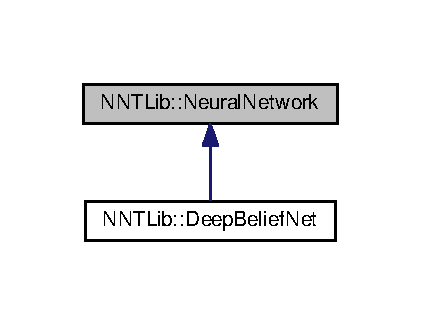
\includegraphics[width=202pt]{class_n_n_t_lib_1_1_neural_network__inherit__graph}
\end{center}
\end{figure}


Collaboration diagram for N\+N\+T\+Lib\+:\+:Neural\+Network\+:\nopagebreak
\begin{figure}[H]
\begin{center}
\leavevmode
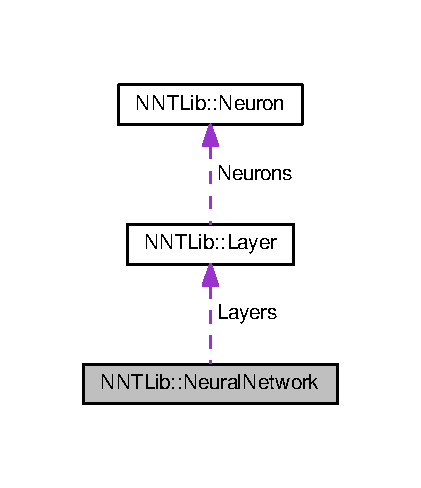
\includegraphics[width=202pt]{class_n_n_t_lib_1_1_neural_network__coll__graph}
\end{center}
\end{figure}
\subsection*{Public Member Functions}
\begin{DoxyCompactItemize}
\item 
\hyperlink{class_n_n_t_lib_1_1_neural_network_ab49cda4bda3cba756cb206727e429ebd}{Neural\+Network} (int $\ast$layers, int layercount, Weight\+Init\+Enum init\+Type, Function\+Enum function\+Type)
\begin{DoxyCompactList}\small\item\em Initializes a new instance of the \hyperlink{class_n_n_t_lib_1_1_neural_network}{Neural\+Network} class. \end{DoxyCompactList}\item 
\hyperlink{class_n_n_t_lib_1_1_neural_network_a634613b66f5441f58a2e5d7c7b1c3da9}{$\sim$\+Neural\+Network} ()
\begin{DoxyCompactList}\small\item\em Finalizes an instance of the \hyperlink{class_n_n_t_lib_1_1_neural_network}{Neural\+Network} class. \end{DoxyCompactList}\item 
\hyperlink{class_n_n_t_lib_1_1_neural_network_a21c3863f38585268af2532b027a42d6b}{Neural\+Network} (const \hyperlink{class_n_n_t_lib_1_1_neural_network}{Neural\+Network} \&that)
\begin{DoxyCompactList}\small\item\em Initializes a new instance of the \hyperlink{class_n_n_t_lib_1_1_neural_network}{Neural\+Network} class. \end{DoxyCompactList}\item 
\hyperlink{class_n_n_t_lib_1_1_neural_network}{Neural\+Network} \& \hyperlink{class_n_n_t_lib_1_1_neural_network_add5684447063d835c50ec511a5f28091}{operator=} (const \hyperlink{class_n_n_t_lib_1_1_neural_network}{Neural\+Network} \&that)
\begin{DoxyCompactList}\small\item\em Operator=s the specified that. \end{DoxyCompactList}\item 
bool \hyperlink{class_n_n_t_lib_1_1_neural_network_a147a7fe89871c02c6fa8c9d691327e0e}{operator$<$} (const \hyperlink{class_n_n_t_lib_1_1_neural_network}{Neural\+Network} \&net) const 
\begin{DoxyCompactList}\small\item\em Operators the specified net. \end{DoxyCompactList}\item 
void \hyperlink{class_n_n_t_lib_1_1_neural_network_a9c9aa74920e9b369d434256c6706e75a}{Init\+Weights} (Weight\+Init\+Enum init\+Type)
\begin{DoxyCompactList}\small\item\em Initializes the weights. \end{DoxyCompactList}\item 
double \hyperlink{class_n_n_t_lib_1_1_neural_network_aee9c78b90d25b0ebb1b3cb3cf732e4fc}{Generate\+Random\+Weight} (int weight\+Count)
\begin{DoxyCompactList}\small\item\em Generates the random weight. \end{DoxyCompactList}\item 
void \hyperlink{class_n_n_t_lib_1_1_neural_network_a4a85f90af22f14e8cce248d9b6e3516c}{Save\+Weights} (const std\+::string file)
\begin{DoxyCompactList}\small\item\em Saves the weights. \end{DoxyCompactList}\item 
void \hyperlink{class_n_n_t_lib_1_1_neural_network_a9c2f594b5aafa05970a47df983436540}{Load\+Weights} (const std\+::string file)
\begin{DoxyCompactList}\small\item\em Loads the weights. \end{DoxyCompactList}\item 
void \hyperlink{class_n_n_t_lib_1_1_neural_network_a86d77108c0d47b6e6dd33dccfef6521f}{Propagate} (const double $\ast$input)
\begin{DoxyCompactList}\small\item\em Propagates the specified input. \end{DoxyCompactList}\item 
void \hyperlink{class_n_n_t_lib_1_1_neural_network_a43e8b626150530fcb8e17aa957ef1d62}{Calculate\+M\+S\+E} (const \hyperlink{class_n_n_t_lib_1_1_data_container}{Data\+Container} \&data)
\begin{DoxyCompactList}\small\item\em Calculates the mse. \end{DoxyCompactList}\end{DoxyCompactItemize}
\subsection*{Public Attributes}
\begin{DoxyCompactItemize}
\item 
int \hyperlink{class_n_n_t_lib_1_1_neural_network_a279ecd5cdb00a4fd3485d7c1366d1ada}{Layers\+Count}
\begin{DoxyCompactList}\small\item\em The layers count \end{DoxyCompactList}\item 
double \hyperlink{class_n_n_t_lib_1_1_neural_network_aa81b59c0bab012cc65f37cfc8870fb7c}{Mean\+Square\+Error}
\begin{DoxyCompactList}\small\item\em The mean square error \end{DoxyCompactList}\item 
Weight\+Init\+Enum \hyperlink{class_n_n_t_lib_1_1_neural_network_aef757cbe4d01525f99125716f217135d}{Weight\+Init\+Type}
\begin{DoxyCompactList}\small\item\em The weight initialize type \end{DoxyCompactList}\item 
Function\+Enum \hyperlink{class_n_n_t_lib_1_1_neural_network_afe71db7f776309201ae3a793d1fcadf8}{Function\+Type}
\begin{DoxyCompactList}\small\item\em The function type \end{DoxyCompactList}\item 
int \hyperlink{class_n_n_t_lib_1_1_neural_network_aeb06dfbd4762d8ce321f7e21532bdad7}{Total\+Neuron\+Count}
\begin{DoxyCompactList}\small\item\em The total neuron count \end{DoxyCompactList}\item 
\hyperlink{class_n_n_t_lib_1_1_layer}{Layer} $\ast$ \hyperlink{class_n_n_t_lib_1_1_neural_network_aa0390db1a1aa19da2b9b205a4572eacd}{Layers}
\begin{DoxyCompactList}\small\item\em The layers \end{DoxyCompactList}\end{DoxyCompactItemize}
\subsection*{Protected Member Functions}
\begin{DoxyCompactItemize}
\item 
void \hyperlink{class_n_n_t_lib_1_1_neural_network_af5d47358b8619b32506b77b916bc8d5c}{copy} (const \hyperlink{class_n_n_t_lib_1_1_neural_network}{Neural\+Network} \&that)
\begin{DoxyCompactList}\small\item\em Copies the specified that. \end{DoxyCompactList}\item 
void \hyperlink{class_n_n_t_lib_1_1_neural_network_a84ad44405463ad6f869525b81447e46d}{init} ()
\begin{DoxyCompactList}\small\item\em Initializes this instance. \end{DoxyCompactList}\item 
void \hyperlink{class_n_n_t_lib_1_1_neural_network_ad9a5359eb94a5358d5813e45e35b7b2d}{free\+Mem} ()
\begin{DoxyCompactList}\small\item\em Frees the memory. \end{DoxyCompactList}\end{DoxyCompactItemize}
\subsection*{Protected Attributes}
\begin{DoxyCompactItemize}
\item 
\hypertarget{class_n_n_t_lib_1_1_neural_network_a12f68bf955726ebafa4020d10b4284b6}{}std\+::mt19937 {\bfseries generator}\label{class_n_n_t_lib_1_1_neural_network_a12f68bf955726ebafa4020d10b4284b6}

\end{DoxyCompactItemize}


\subsection{Constructor \& Destructor Documentation}
\hypertarget{class_n_n_t_lib_1_1_neural_network_ab49cda4bda3cba756cb206727e429ebd}{}\index{N\+N\+T\+Lib\+::\+Neural\+Network@{N\+N\+T\+Lib\+::\+Neural\+Network}!Neural\+Network@{Neural\+Network}}
\index{Neural\+Network@{Neural\+Network}!N\+N\+T\+Lib\+::\+Neural\+Network@{N\+N\+T\+Lib\+::\+Neural\+Network}}
\subsubsection[{Neural\+Network}]{\setlength{\rightskip}{0pt plus 5cm}N\+N\+T\+Lib\+::\+Neural\+Network\+::\+Neural\+Network (
\begin{DoxyParamCaption}
\item[{int $\ast$}]{neurons\+Count\+Per\+Layer, }
\item[{int}]{layercount, }
\item[{Weight\+Init\+Enum}]{init\+Type, }
\item[{Function\+Enum}]{function\+Type}
\end{DoxyParamCaption}
)}\label{class_n_n_t_lib_1_1_neural_network_ab49cda4bda3cba756cb206727e429ebd}


Initializes a new instance of the \hyperlink{class_n_n_t_lib_1_1_neural_network}{Neural\+Network} class. 


\begin{DoxyParams}{Parameters}
{\em neurons\+Count\+Per\+Layer} & The hidden layers.\\
\hline
{\em layercount} & The hidden layercount.\\
\hline
{\em init\+Type} & Type of the initialize.\\
\hline
{\em function\+Type} & Type of the function.\\
\hline
\end{DoxyParams}
\hypertarget{class_n_n_t_lib_1_1_neural_network_a634613b66f5441f58a2e5d7c7b1c3da9}{}\index{N\+N\+T\+Lib\+::\+Neural\+Network@{N\+N\+T\+Lib\+::\+Neural\+Network}!````~Neural\+Network@{$\sim$\+Neural\+Network}}
\index{````~Neural\+Network@{$\sim$\+Neural\+Network}!N\+N\+T\+Lib\+::\+Neural\+Network@{N\+N\+T\+Lib\+::\+Neural\+Network}}
\subsubsection[{$\sim$\+Neural\+Network}]{\setlength{\rightskip}{0pt plus 5cm}N\+N\+T\+Lib\+::\+Neural\+Network\+::$\sim$\+Neural\+Network (
\begin{DoxyParamCaption}
{}
\end{DoxyParamCaption}
)}\label{class_n_n_t_lib_1_1_neural_network_a634613b66f5441f58a2e5d7c7b1c3da9}


Finalizes an instance of the \hyperlink{class_n_n_t_lib_1_1_neural_network}{Neural\+Network} class. 

\hypertarget{class_n_n_t_lib_1_1_neural_network_a21c3863f38585268af2532b027a42d6b}{}\index{N\+N\+T\+Lib\+::\+Neural\+Network@{N\+N\+T\+Lib\+::\+Neural\+Network}!Neural\+Network@{Neural\+Network}}
\index{Neural\+Network@{Neural\+Network}!N\+N\+T\+Lib\+::\+Neural\+Network@{N\+N\+T\+Lib\+::\+Neural\+Network}}
\subsubsection[{Neural\+Network}]{\setlength{\rightskip}{0pt plus 5cm}N\+N\+T\+Lib\+::\+Neural\+Network\+::\+Neural\+Network (
\begin{DoxyParamCaption}
\item[{const {\bf Neural\+Network} \&}]{that}
\end{DoxyParamCaption}
)}\label{class_n_n_t_lib_1_1_neural_network_a21c3863f38585268af2532b027a42d6b}


Initializes a new instance of the \hyperlink{class_n_n_t_lib_1_1_neural_network}{Neural\+Network} class. 


\begin{DoxyParams}{Parameters}
{\em that} & The that.\\
\hline
\end{DoxyParams}


\subsection{Member Function Documentation}
\hypertarget{class_n_n_t_lib_1_1_neural_network_a43e8b626150530fcb8e17aa957ef1d62}{}\index{N\+N\+T\+Lib\+::\+Neural\+Network@{N\+N\+T\+Lib\+::\+Neural\+Network}!Calculate\+M\+S\+E@{Calculate\+M\+S\+E}}
\index{Calculate\+M\+S\+E@{Calculate\+M\+S\+E}!N\+N\+T\+Lib\+::\+Neural\+Network@{N\+N\+T\+Lib\+::\+Neural\+Network}}
\subsubsection[{Calculate\+M\+S\+E}]{\setlength{\rightskip}{0pt plus 5cm}void N\+N\+T\+Lib\+::\+Neural\+Network\+::\+Calculate\+M\+S\+E (
\begin{DoxyParamCaption}
\item[{const {\bf Data\+Container} \&}]{data}
\end{DoxyParamCaption}
)}\label{class_n_n_t_lib_1_1_neural_network_a43e8b626150530fcb8e17aa957ef1d62}


Calculates the mse. 


\begin{DoxyParams}{Parameters}
{\em data} & The data.\\
\hline
\end{DoxyParams}
\hypertarget{class_n_n_t_lib_1_1_neural_network_af5d47358b8619b32506b77b916bc8d5c}{}\index{N\+N\+T\+Lib\+::\+Neural\+Network@{N\+N\+T\+Lib\+::\+Neural\+Network}!copy@{copy}}
\index{copy@{copy}!N\+N\+T\+Lib\+::\+Neural\+Network@{N\+N\+T\+Lib\+::\+Neural\+Network}}
\subsubsection[{copy}]{\setlength{\rightskip}{0pt plus 5cm}void N\+N\+T\+Lib\+::\+Neural\+Network\+::copy (
\begin{DoxyParamCaption}
\item[{const {\bf Neural\+Network} \&}]{that}
\end{DoxyParamCaption}
)\hspace{0.3cm}{\ttfamily [protected]}}\label{class_n_n_t_lib_1_1_neural_network_af5d47358b8619b32506b77b916bc8d5c}


Copies the specified that. 


\begin{DoxyParams}{Parameters}
{\em that} & The that.\\
\hline
\end{DoxyParams}
\hypertarget{class_n_n_t_lib_1_1_neural_network_ad9a5359eb94a5358d5813e45e35b7b2d}{}\index{N\+N\+T\+Lib\+::\+Neural\+Network@{N\+N\+T\+Lib\+::\+Neural\+Network}!free\+Mem@{free\+Mem}}
\index{free\+Mem@{free\+Mem}!N\+N\+T\+Lib\+::\+Neural\+Network@{N\+N\+T\+Lib\+::\+Neural\+Network}}
\subsubsection[{free\+Mem}]{\setlength{\rightskip}{0pt plus 5cm}void N\+N\+T\+Lib\+::\+Neural\+Network\+::free\+Mem (
\begin{DoxyParamCaption}
{}
\end{DoxyParamCaption}
)\hspace{0.3cm}{\ttfamily [protected]}}\label{class_n_n_t_lib_1_1_neural_network_ad9a5359eb94a5358d5813e45e35b7b2d}


Frees the memory. 

\hypertarget{class_n_n_t_lib_1_1_neural_network_aee9c78b90d25b0ebb1b3cb3cf732e4fc}{}\index{N\+N\+T\+Lib\+::\+Neural\+Network@{N\+N\+T\+Lib\+::\+Neural\+Network}!Generate\+Random\+Weight@{Generate\+Random\+Weight}}
\index{Generate\+Random\+Weight@{Generate\+Random\+Weight}!N\+N\+T\+Lib\+::\+Neural\+Network@{N\+N\+T\+Lib\+::\+Neural\+Network}}
\subsubsection[{Generate\+Random\+Weight}]{\setlength{\rightskip}{0pt plus 5cm}double N\+N\+T\+Lib\+::\+Neural\+Network\+::\+Generate\+Random\+Weight (
\begin{DoxyParamCaption}
\item[{int}]{weight\+Count}
\end{DoxyParamCaption}
)}\label{class_n_n_t_lib_1_1_neural_network_aee9c78b90d25b0ebb1b3cb3cf732e4fc}


Generates the random weight. 


\begin{DoxyParams}{Parameters}
{\em input\+Vector\+Count\+With\+Bias} & The input vector count with bias.\\
\hline
\end{DoxyParams}
\begin{DoxyReturn}{Returns}

\end{DoxyReturn}
\hypertarget{class_n_n_t_lib_1_1_neural_network_a84ad44405463ad6f869525b81447e46d}{}\index{N\+N\+T\+Lib\+::\+Neural\+Network@{N\+N\+T\+Lib\+::\+Neural\+Network}!init@{init}}
\index{init@{init}!N\+N\+T\+Lib\+::\+Neural\+Network@{N\+N\+T\+Lib\+::\+Neural\+Network}}
\subsubsection[{init}]{\setlength{\rightskip}{0pt plus 5cm}void N\+N\+T\+Lib\+::\+Neural\+Network\+::init (
\begin{DoxyParamCaption}
{}
\end{DoxyParamCaption}
)\hspace{0.3cm}{\ttfamily [protected]}}\label{class_n_n_t_lib_1_1_neural_network_a84ad44405463ad6f869525b81447e46d}


Initializes this instance. 

\hypertarget{class_n_n_t_lib_1_1_neural_network_a9c9aa74920e9b369d434256c6706e75a}{}\index{N\+N\+T\+Lib\+::\+Neural\+Network@{N\+N\+T\+Lib\+::\+Neural\+Network}!Init\+Weights@{Init\+Weights}}
\index{Init\+Weights@{Init\+Weights}!N\+N\+T\+Lib\+::\+Neural\+Network@{N\+N\+T\+Lib\+::\+Neural\+Network}}
\subsubsection[{Init\+Weights}]{\setlength{\rightskip}{0pt plus 5cm}void N\+N\+T\+Lib\+::\+Neural\+Network\+::\+Init\+Weights (
\begin{DoxyParamCaption}
\item[{Weight\+Init\+Enum}]{init\+Type}
\end{DoxyParamCaption}
)}\label{class_n_n_t_lib_1_1_neural_network_a9c9aa74920e9b369d434256c6706e75a}


Initializes the weights. 


\begin{DoxyParams}{Parameters}
{\em init\+Type} & Type of the initialize.\\
\hline
\end{DoxyParams}
\hypertarget{class_n_n_t_lib_1_1_neural_network_a9c2f594b5aafa05970a47df983436540}{}\index{N\+N\+T\+Lib\+::\+Neural\+Network@{N\+N\+T\+Lib\+::\+Neural\+Network}!Load\+Weights@{Load\+Weights}}
\index{Load\+Weights@{Load\+Weights}!N\+N\+T\+Lib\+::\+Neural\+Network@{N\+N\+T\+Lib\+::\+Neural\+Network}}
\subsubsection[{Load\+Weights}]{\setlength{\rightskip}{0pt plus 5cm}void N\+N\+T\+Lib\+::\+Neural\+Network\+::\+Load\+Weights (
\begin{DoxyParamCaption}
\item[{const std\+::string}]{file}
\end{DoxyParamCaption}
)}\label{class_n_n_t_lib_1_1_neural_network_a9c2f594b5aafa05970a47df983436540}


Loads the weights. 


\begin{DoxyParams}{Parameters}
{\em file} & The file.\\
\hline
\end{DoxyParams}
\hypertarget{class_n_n_t_lib_1_1_neural_network_a147a7fe89871c02c6fa8c9d691327e0e}{}\index{N\+N\+T\+Lib\+::\+Neural\+Network@{N\+N\+T\+Lib\+::\+Neural\+Network}!operator$<$@{operator$<$}}
\index{operator$<$@{operator$<$}!N\+N\+T\+Lib\+::\+Neural\+Network@{N\+N\+T\+Lib\+::\+Neural\+Network}}
\subsubsection[{operator$<$}]{\setlength{\rightskip}{0pt plus 5cm}bool N\+N\+T\+Lib\+::\+Neural\+Network\+::operator$<$ (
\begin{DoxyParamCaption}
\item[{const {\bf Neural\+Network} \&}]{net}
\end{DoxyParamCaption}
) const}\label{class_n_n_t_lib_1_1_neural_network_a147a7fe89871c02c6fa8c9d691327e0e}


Operators the specified net. 


\begin{DoxyParams}{Parameters}
{\em net} & The net.\\
\hline
\end{DoxyParams}
\begin{DoxyReturn}{Returns}

\end{DoxyReturn}
\hypertarget{class_n_n_t_lib_1_1_neural_network_add5684447063d835c50ec511a5f28091}{}\index{N\+N\+T\+Lib\+::\+Neural\+Network@{N\+N\+T\+Lib\+::\+Neural\+Network}!operator=@{operator=}}
\index{operator=@{operator=}!N\+N\+T\+Lib\+::\+Neural\+Network@{N\+N\+T\+Lib\+::\+Neural\+Network}}
\subsubsection[{operator=}]{\setlength{\rightskip}{0pt plus 5cm}{\bf Neural\+Network} \& N\+N\+T\+Lib\+::\+Neural\+Network\+::operator= (
\begin{DoxyParamCaption}
\item[{const {\bf Neural\+Network} \&}]{that}
\end{DoxyParamCaption}
)}\label{class_n_n_t_lib_1_1_neural_network_add5684447063d835c50ec511a5f28091}


Operator=s the specified that. 


\begin{DoxyParams}{Parameters}
{\em that} & The that.\\
\hline
\end{DoxyParams}
\begin{DoxyReturn}{Returns}

\end{DoxyReturn}
\hypertarget{class_n_n_t_lib_1_1_neural_network_a86d77108c0d47b6e6dd33dccfef6521f}{}\index{N\+N\+T\+Lib\+::\+Neural\+Network@{N\+N\+T\+Lib\+::\+Neural\+Network}!Propagate@{Propagate}}
\index{Propagate@{Propagate}!N\+N\+T\+Lib\+::\+Neural\+Network@{N\+N\+T\+Lib\+::\+Neural\+Network}}
\subsubsection[{Propagate}]{\setlength{\rightskip}{0pt plus 5cm}void N\+N\+T\+Lib\+::\+Neural\+Network\+::\+Propagate (
\begin{DoxyParamCaption}
\item[{const double $\ast$}]{input}
\end{DoxyParamCaption}
)}\label{class_n_n_t_lib_1_1_neural_network_a86d77108c0d47b6e6dd33dccfef6521f}


Propagates the specified input. 


\begin{DoxyParams}{Parameters}
{\em input} & The input.\\
\hline
\end{DoxyParams}
neuron-\/$>$Bias \hypertarget{class_n_n_t_lib_1_1_neural_network_a4a85f90af22f14e8cce248d9b6e3516c}{}\index{N\+N\+T\+Lib\+::\+Neural\+Network@{N\+N\+T\+Lib\+::\+Neural\+Network}!Save\+Weights@{Save\+Weights}}
\index{Save\+Weights@{Save\+Weights}!N\+N\+T\+Lib\+::\+Neural\+Network@{N\+N\+T\+Lib\+::\+Neural\+Network}}
\subsubsection[{Save\+Weights}]{\setlength{\rightskip}{0pt plus 5cm}void N\+N\+T\+Lib\+::\+Neural\+Network\+::\+Save\+Weights (
\begin{DoxyParamCaption}
\item[{const std\+::string}]{file}
\end{DoxyParamCaption}
)}\label{class_n_n_t_lib_1_1_neural_network_a4a85f90af22f14e8cce248d9b6e3516c}


Saves the weights. 


\begin{DoxyParams}{Parameters}
{\em file} & The file.\\
\hline
\end{DoxyParams}


\subsection{Member Data Documentation}
\hypertarget{class_n_n_t_lib_1_1_neural_network_afe71db7f776309201ae3a793d1fcadf8}{}\index{N\+N\+T\+Lib\+::\+Neural\+Network@{N\+N\+T\+Lib\+::\+Neural\+Network}!Function\+Type@{Function\+Type}}
\index{Function\+Type@{Function\+Type}!N\+N\+T\+Lib\+::\+Neural\+Network@{N\+N\+T\+Lib\+::\+Neural\+Network}}
\subsubsection[{Function\+Type}]{\setlength{\rightskip}{0pt plus 5cm}Function\+Enum N\+N\+T\+Lib\+::\+Neural\+Network\+::\+Function\+Type}\label{class_n_n_t_lib_1_1_neural_network_afe71db7f776309201ae3a793d1fcadf8}


The function type 

\hypertarget{class_n_n_t_lib_1_1_neural_network_aa0390db1a1aa19da2b9b205a4572eacd}{}\index{N\+N\+T\+Lib\+::\+Neural\+Network@{N\+N\+T\+Lib\+::\+Neural\+Network}!Layers@{Layers}}
\index{Layers@{Layers}!N\+N\+T\+Lib\+::\+Neural\+Network@{N\+N\+T\+Lib\+::\+Neural\+Network}}
\subsubsection[{Layers}]{\setlength{\rightskip}{0pt plus 5cm}{\bf Layer}$\ast$ N\+N\+T\+Lib\+::\+Neural\+Network\+::\+Layers}\label{class_n_n_t_lib_1_1_neural_network_aa0390db1a1aa19da2b9b205a4572eacd}


The layers 

\hypertarget{class_n_n_t_lib_1_1_neural_network_a279ecd5cdb00a4fd3485d7c1366d1ada}{}\index{N\+N\+T\+Lib\+::\+Neural\+Network@{N\+N\+T\+Lib\+::\+Neural\+Network}!Layers\+Count@{Layers\+Count}}
\index{Layers\+Count@{Layers\+Count}!N\+N\+T\+Lib\+::\+Neural\+Network@{N\+N\+T\+Lib\+::\+Neural\+Network}}
\subsubsection[{Layers\+Count}]{\setlength{\rightskip}{0pt plus 5cm}int N\+N\+T\+Lib\+::\+Neural\+Network\+::\+Layers\+Count}\label{class_n_n_t_lib_1_1_neural_network_a279ecd5cdb00a4fd3485d7c1366d1ada}


The layers count 

\hypertarget{class_n_n_t_lib_1_1_neural_network_aa81b59c0bab012cc65f37cfc8870fb7c}{}\index{N\+N\+T\+Lib\+::\+Neural\+Network@{N\+N\+T\+Lib\+::\+Neural\+Network}!Mean\+Square\+Error@{Mean\+Square\+Error}}
\index{Mean\+Square\+Error@{Mean\+Square\+Error}!N\+N\+T\+Lib\+::\+Neural\+Network@{N\+N\+T\+Lib\+::\+Neural\+Network}}
\subsubsection[{Mean\+Square\+Error}]{\setlength{\rightskip}{0pt plus 5cm}double N\+N\+T\+Lib\+::\+Neural\+Network\+::\+Mean\+Square\+Error}\label{class_n_n_t_lib_1_1_neural_network_aa81b59c0bab012cc65f37cfc8870fb7c}


The mean square error 

\hypertarget{class_n_n_t_lib_1_1_neural_network_aeb06dfbd4762d8ce321f7e21532bdad7}{}\index{N\+N\+T\+Lib\+::\+Neural\+Network@{N\+N\+T\+Lib\+::\+Neural\+Network}!Total\+Neuron\+Count@{Total\+Neuron\+Count}}
\index{Total\+Neuron\+Count@{Total\+Neuron\+Count}!N\+N\+T\+Lib\+::\+Neural\+Network@{N\+N\+T\+Lib\+::\+Neural\+Network}}
\subsubsection[{Total\+Neuron\+Count}]{\setlength{\rightskip}{0pt plus 5cm}int N\+N\+T\+Lib\+::\+Neural\+Network\+::\+Total\+Neuron\+Count}\label{class_n_n_t_lib_1_1_neural_network_aeb06dfbd4762d8ce321f7e21532bdad7}


The total neuron count 

\hypertarget{class_n_n_t_lib_1_1_neural_network_aef757cbe4d01525f99125716f217135d}{}\index{N\+N\+T\+Lib\+::\+Neural\+Network@{N\+N\+T\+Lib\+::\+Neural\+Network}!Weight\+Init\+Type@{Weight\+Init\+Type}}
\index{Weight\+Init\+Type@{Weight\+Init\+Type}!N\+N\+T\+Lib\+::\+Neural\+Network@{N\+N\+T\+Lib\+::\+Neural\+Network}}
\subsubsection[{Weight\+Init\+Type}]{\setlength{\rightskip}{0pt plus 5cm}Weight\+Init\+Enum N\+N\+T\+Lib\+::\+Neural\+Network\+::\+Weight\+Init\+Type}\label{class_n_n_t_lib_1_1_neural_network_aef757cbe4d01525f99125716f217135d}


The weight initialize type 



The documentation for this class was generated from the following files\+:\begin{DoxyCompactItemize}
\item 
N\+N\+T\+Lib/Neural\+Network.\+h\item 
N\+N\+T\+Lib/Neural\+Network.\+cpp\end{DoxyCompactItemize}

\hypertarget{class_neural_network_config}{}\section{Neural\+Network\+Config Class Reference}
\label{class_neural_network_config}\index{Neural\+Network\+Config@{Neural\+Network\+Config}}


Inheritance diagram for Neural\+Network\+Config\+:\nopagebreak
\begin{figure}[H]
\begin{center}
\leavevmode
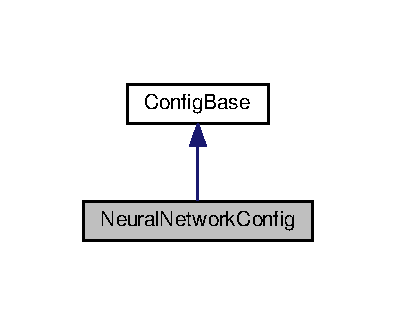
\includegraphics[width=190pt]{class_neural_network_config__inherit__graph}
\end{center}
\end{figure}


Collaboration diagram for Neural\+Network\+Config\+:\nopagebreak
\begin{figure}[H]
\begin{center}
\leavevmode
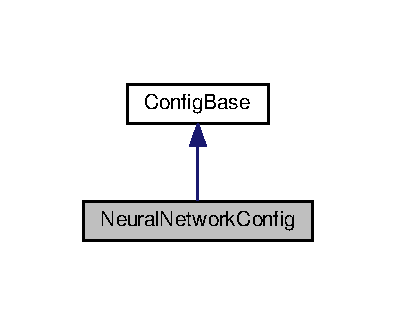
\includegraphics[width=190pt]{class_neural_network_config__coll__graph}
\end{center}
\end{figure}
\subsection*{Public Member Functions}
\begin{DoxyCompactItemize}
\item 
\hyperlink{class_neural_network_config_aac0a64831aa0011542cd0da2621b3e38}{Neural\+Network\+Config} ()
\begin{DoxyCompactList}\small\item\em Initializes a new instance of the \hyperlink{class_neural_network_config}{Neural\+Network\+Config} class. \end{DoxyCompactList}\item 
\hyperlink{class_neural_network_config_a311624b119b714c5282f00f5bbcff53c}{$\sim$\+Neural\+Network\+Config} ()
\begin{DoxyCompactList}\small\item\em Finalizes an instance of the \hyperlink{class_neural_network_config}{Neural\+Network\+Config} class. \end{DoxyCompactList}\item 
\hyperlink{class_neural_network_config_a6b6dc46d5fd9243c781e71b021dbb5ca}{Neural\+Network\+Config} (const \hyperlink{class_neural_network_config}{Neural\+Network\+Config} \&that)
\begin{DoxyCompactList}\small\item\em Initializes a new instance of the \hyperlink{class_neural_network_config}{Neural\+Network\+Config} class. \end{DoxyCompactList}\item 
\hyperlink{class_neural_network_config}{Neural\+Network\+Config} \& \hyperlink{class_neural_network_config_a17075aa3c368ec77e49902eda3bcff7b}{operator=} (const \hyperlink{class_neural_network_config}{Neural\+Network\+Config} \&that)
\begin{DoxyCompactList}\small\item\em Operator=s the specified that. \end{DoxyCompactList}\item 
void \hyperlink{class_neural_network_config_ace2d78217b376541455866a7360277c5}{Print\+Data} ()
\begin{DoxyCompactList}\small\item\em Prints the data. \end{DoxyCompactList}\item 
bool \hyperlink{class_neural_network_config_a3975927f8a58d466c19a791537860e55}{Is\+Config\+Valid} ()
\begin{DoxyCompactList}\small\item\em Determines whether \mbox{[}is configuration valid\mbox{]}. \end{DoxyCompactList}\end{DoxyCompactItemize}
\subsection*{Public Attributes}
\begin{DoxyCompactItemize}
\item 
int \hyperlink{class_neural_network_config_a1bbbe016a258c2ac3fb52e1e4873ca38}{Layer\+Count}
\begin{DoxyCompactList}\small\item\em The layer count \end{DoxyCompactList}\item 
N\+N\+T\+Lib\+::\+Function\+Enum \hyperlink{class_neural_network_config_a41262125abc80afb0e32470468a7afb0}{Function\+Type}
\begin{DoxyCompactList}\small\item\em The function type \end{DoxyCompactList}\item 
N\+N\+T\+Lib\+::\+Weight\+Init\+Enum \hyperlink{class_neural_network_config_ac387c49af177bd1c2d122fdab2250ea3}{Weight\+Init\+Type}
\begin{DoxyCompactList}\small\item\em The weight initialize type \end{DoxyCompactList}\item 
int $\ast$ \hyperlink{class_neural_network_config_a86a494523f269a122a439144c9e6cb89}{Layer\+Neuron\+Count}
\begin{DoxyCompactList}\small\item\em The layer neuron count \end{DoxyCompactList}\end{DoxyCompactItemize}
\subsection*{Protected Member Functions}
\begin{DoxyCompactItemize}
\item 
void \hyperlink{class_neural_network_config_ac913258430c16d29912c2882c8350bcd}{Handle\+Name\+Value} (std\+::string name, std\+::string value)
\begin{DoxyCompactList}\small\item\em Handles the name value. \end{DoxyCompactList}\end{DoxyCompactItemize}


\subsection{Constructor \& Destructor Documentation}
\hypertarget{class_neural_network_config_aac0a64831aa0011542cd0da2621b3e38}{}\index{Neural\+Network\+Config@{Neural\+Network\+Config}!Neural\+Network\+Config@{Neural\+Network\+Config}}
\index{Neural\+Network\+Config@{Neural\+Network\+Config}!Neural\+Network\+Config@{Neural\+Network\+Config}}
\subsubsection[{Neural\+Network\+Config}]{\setlength{\rightskip}{0pt plus 5cm}Neural\+Network\+Config\+::\+Neural\+Network\+Config (
\begin{DoxyParamCaption}
{}
\end{DoxyParamCaption}
)}\label{class_neural_network_config_aac0a64831aa0011542cd0da2621b3e38}


Initializes a new instance of the \hyperlink{class_neural_network_config}{Neural\+Network\+Config} class. 

\hypertarget{class_neural_network_config_a311624b119b714c5282f00f5bbcff53c}{}\index{Neural\+Network\+Config@{Neural\+Network\+Config}!````~Neural\+Network\+Config@{$\sim$\+Neural\+Network\+Config}}
\index{````~Neural\+Network\+Config@{$\sim$\+Neural\+Network\+Config}!Neural\+Network\+Config@{Neural\+Network\+Config}}
\subsubsection[{$\sim$\+Neural\+Network\+Config}]{\setlength{\rightskip}{0pt plus 5cm}Neural\+Network\+Config\+::$\sim$\+Neural\+Network\+Config (
\begin{DoxyParamCaption}
{}
\end{DoxyParamCaption}
)}\label{class_neural_network_config_a311624b119b714c5282f00f5bbcff53c}


Finalizes an instance of the \hyperlink{class_neural_network_config}{Neural\+Network\+Config} class. 

\hypertarget{class_neural_network_config_a6b6dc46d5fd9243c781e71b021dbb5ca}{}\index{Neural\+Network\+Config@{Neural\+Network\+Config}!Neural\+Network\+Config@{Neural\+Network\+Config}}
\index{Neural\+Network\+Config@{Neural\+Network\+Config}!Neural\+Network\+Config@{Neural\+Network\+Config}}
\subsubsection[{Neural\+Network\+Config}]{\setlength{\rightskip}{0pt plus 5cm}Neural\+Network\+Config\+::\+Neural\+Network\+Config (
\begin{DoxyParamCaption}
\item[{const {\bf Neural\+Network\+Config} \&}]{that}
\end{DoxyParamCaption}
)}\label{class_neural_network_config_a6b6dc46d5fd9243c781e71b021dbb5ca}


Initializes a new instance of the \hyperlink{class_neural_network_config}{Neural\+Network\+Config} class. 


\begin{DoxyParams}{Parameters}
{\em that} & The that.\\
\hline
\end{DoxyParams}


\subsection{Member Function Documentation}
\hypertarget{class_neural_network_config_ac913258430c16d29912c2882c8350bcd}{}\index{Neural\+Network\+Config@{Neural\+Network\+Config}!Handle\+Name\+Value@{Handle\+Name\+Value}}
\index{Handle\+Name\+Value@{Handle\+Name\+Value}!Neural\+Network\+Config@{Neural\+Network\+Config}}
\subsubsection[{Handle\+Name\+Value}]{\setlength{\rightskip}{0pt plus 5cm}void Neural\+Network\+Config\+::\+Handle\+Name\+Value (
\begin{DoxyParamCaption}
\item[{std\+::string}]{name, }
\item[{std\+::string}]{value}
\end{DoxyParamCaption}
)\hspace{0.3cm}{\ttfamily [protected]}, {\ttfamily [virtual]}}\label{class_neural_network_config_ac913258430c16d29912c2882c8350bcd}


Handles the name value. 


\begin{DoxyParams}{Parameters}
{\em name} & The name.\\
\hline
{\em value} & The value.\\
\hline
\end{DoxyParams}


Implements \hyperlink{class_config_base}{Config\+Base}.

\hypertarget{class_neural_network_config_a3975927f8a58d466c19a791537860e55}{}\index{Neural\+Network\+Config@{Neural\+Network\+Config}!Is\+Config\+Valid@{Is\+Config\+Valid}}
\index{Is\+Config\+Valid@{Is\+Config\+Valid}!Neural\+Network\+Config@{Neural\+Network\+Config}}
\subsubsection[{Is\+Config\+Valid}]{\setlength{\rightskip}{0pt plus 5cm}bool Neural\+Network\+Config\+::\+Is\+Config\+Valid (
\begin{DoxyParamCaption}
{}
\end{DoxyParamCaption}
)\hspace{0.3cm}{\ttfamily [virtual]}}\label{class_neural_network_config_a3975927f8a58d466c19a791537860e55}


Determines whether \mbox{[}is configuration valid\mbox{]}. 

\begin{DoxyReturn}{Returns}

\end{DoxyReturn}


Implements \hyperlink{class_config_base}{Config\+Base}.

\hypertarget{class_neural_network_config_a17075aa3c368ec77e49902eda3bcff7b}{}\index{Neural\+Network\+Config@{Neural\+Network\+Config}!operator=@{operator=}}
\index{operator=@{operator=}!Neural\+Network\+Config@{Neural\+Network\+Config}}
\subsubsection[{operator=}]{\setlength{\rightskip}{0pt plus 5cm}{\bf Neural\+Network\+Config} \& Neural\+Network\+Config\+::operator= (
\begin{DoxyParamCaption}
\item[{const {\bf Neural\+Network\+Config} \&}]{that}
\end{DoxyParamCaption}
)}\label{class_neural_network_config_a17075aa3c368ec77e49902eda3bcff7b}


Operator=s the specified that. 


\begin{DoxyParams}{Parameters}
{\em that} & The that.\\
\hline
\end{DoxyParams}
\begin{DoxyReturn}{Returns}

\end{DoxyReturn}
\hypertarget{class_neural_network_config_ace2d78217b376541455866a7360277c5}{}\index{Neural\+Network\+Config@{Neural\+Network\+Config}!Print\+Data@{Print\+Data}}
\index{Print\+Data@{Print\+Data}!Neural\+Network\+Config@{Neural\+Network\+Config}}
\subsubsection[{Print\+Data}]{\setlength{\rightskip}{0pt plus 5cm}void Neural\+Network\+Config\+::\+Print\+Data (
\begin{DoxyParamCaption}
{}
\end{DoxyParamCaption}
)\hspace{0.3cm}{\ttfamily [virtual]}}\label{class_neural_network_config_ace2d78217b376541455866a7360277c5}


Prints the data. 



Implements \hyperlink{class_config_base}{Config\+Base}.



\subsection{Member Data Documentation}
\hypertarget{class_neural_network_config_a41262125abc80afb0e32470468a7afb0}{}\index{Neural\+Network\+Config@{Neural\+Network\+Config}!Function\+Type@{Function\+Type}}
\index{Function\+Type@{Function\+Type}!Neural\+Network\+Config@{Neural\+Network\+Config}}
\subsubsection[{Function\+Type}]{\setlength{\rightskip}{0pt plus 5cm}N\+N\+T\+Lib\+::\+Function\+Enum Neural\+Network\+Config\+::\+Function\+Type}\label{class_neural_network_config_a41262125abc80afb0e32470468a7afb0}


The function type 

\hypertarget{class_neural_network_config_a1bbbe016a258c2ac3fb52e1e4873ca38}{}\index{Neural\+Network\+Config@{Neural\+Network\+Config}!Layer\+Count@{Layer\+Count}}
\index{Layer\+Count@{Layer\+Count}!Neural\+Network\+Config@{Neural\+Network\+Config}}
\subsubsection[{Layer\+Count}]{\setlength{\rightskip}{0pt plus 5cm}int Neural\+Network\+Config\+::\+Layer\+Count}\label{class_neural_network_config_a1bbbe016a258c2ac3fb52e1e4873ca38}


The layer count 

\hypertarget{class_neural_network_config_a86a494523f269a122a439144c9e6cb89}{}\index{Neural\+Network\+Config@{Neural\+Network\+Config}!Layer\+Neuron\+Count@{Layer\+Neuron\+Count}}
\index{Layer\+Neuron\+Count@{Layer\+Neuron\+Count}!Neural\+Network\+Config@{Neural\+Network\+Config}}
\subsubsection[{Layer\+Neuron\+Count}]{\setlength{\rightskip}{0pt plus 5cm}int$\ast$ Neural\+Network\+Config\+::\+Layer\+Neuron\+Count}\label{class_neural_network_config_a86a494523f269a122a439144c9e6cb89}


The layer neuron count 

\hypertarget{class_neural_network_config_ac387c49af177bd1c2d122fdab2250ea3}{}\index{Neural\+Network\+Config@{Neural\+Network\+Config}!Weight\+Init\+Type@{Weight\+Init\+Type}}
\index{Weight\+Init\+Type@{Weight\+Init\+Type}!Neural\+Network\+Config@{Neural\+Network\+Config}}
\subsubsection[{Weight\+Init\+Type}]{\setlength{\rightskip}{0pt plus 5cm}N\+N\+T\+Lib\+::\+Weight\+Init\+Enum Neural\+Network\+Config\+::\+Weight\+Init\+Type}\label{class_neural_network_config_ac387c49af177bd1c2d122fdab2250ea3}


The weight initialize type 



The documentation for this class was generated from the following files\+:\begin{DoxyCompactItemize}
\item 
N\+N\+T\+Lib/Neural\+Network\+Config.\+h\item 
N\+N\+T\+Lib/Neural\+Network\+Config.\+cpp\end{DoxyCompactItemize}

\hypertarget{class_n_n_t_lib_1_1_neuron}{}\section{N\+N\+T\+Lib\+:\+:Neuron Class Reference}
\label{class_n_n_t_lib_1_1_neuron}\index{N\+N\+T\+Lib\+::\+Neuron@{N\+N\+T\+Lib\+::\+Neuron}}


Inheritance diagram for N\+N\+T\+Lib\+:\+:Neuron\+:\nopagebreak
\begin{figure}[H]
\begin{center}
\leavevmode
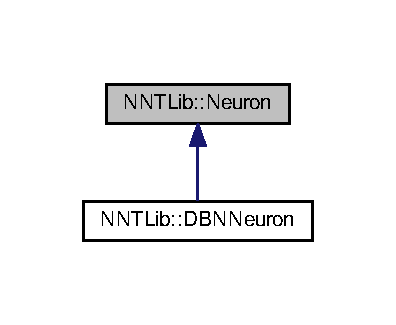
\includegraphics[width=190pt]{class_n_n_t_lib_1_1_neuron__inherit__graph}
\end{center}
\end{figure}
\subsection*{Public Member Functions}
\begin{DoxyCompactItemize}
\item 
\hyperlink{class_n_n_t_lib_1_1_neuron_a0f61ffe37543468f1d91d57b2e932cf5}{Neuron} ()
\begin{DoxyCompactList}\small\item\em Initializes a new instance of the \hyperlink{class_n_n_t_lib_1_1_neuron}{Neuron} class. \end{DoxyCompactList}\item 
\hyperlink{class_n_n_t_lib_1_1_neuron_abd6b77698a485a3f55eea67a49b03f84}{$\sim$\+Neuron} ()
\begin{DoxyCompactList}\small\item\em Finalizes an instance of the \hyperlink{class_n_n_t_lib_1_1_neuron}{Neuron} class. \end{DoxyCompactList}\item 
\hyperlink{class_n_n_t_lib_1_1_neuron_ad99424020cc9a321cd969e0384d2ed59}{Neuron} (const \hyperlink{class_n_n_t_lib_1_1_neuron}{Neuron} \&that)
\begin{DoxyCompactList}\small\item\em Initializes a new instance of the \hyperlink{class_n_n_t_lib_1_1_neuron}{Neuron} class. \end{DoxyCompactList}\item 
\hyperlink{class_n_n_t_lib_1_1_neuron}{Neuron} \& \hyperlink{class_n_n_t_lib_1_1_neuron_a5595c9a7708259b10bd9f7dca47fca2f}{operator=} (const \hyperlink{class_n_n_t_lib_1_1_neuron}{Neuron} \&that)
\begin{DoxyCompactList}\small\item\em Operator=s the specified that. \end{DoxyCompactList}\item 
void \hyperlink{class_n_n_t_lib_1_1_neuron_ada7e263030d3d9bb9ebf15a965e3ce8b}{Init} (int weight\+Count)
\begin{DoxyCompactList}\small\item\em Initializes the specified input vector count. \end{DoxyCompactList}\end{DoxyCompactItemize}
\subsection*{Public Attributes}
\begin{DoxyCompactItemize}
\item 
int \hyperlink{class_n_n_t_lib_1_1_neuron_a61419230ea3df4452d18b4651fc70c15}{Weight\+Count}
\begin{DoxyCompactList}\small\item\em The weight count (Anzahl eingehende Gewichte (mit Schwellenwert) \end{DoxyCompactList}\item 
double \hyperlink{class_n_n_t_lib_1_1_neuron_acb6a45380511787faa355f5104d61f4b}{Output}
\begin{DoxyCompactList}\small\item\em The output (Ausgabe des Neurons) \end{DoxyCompactList}\item 
double $\ast$ \hyperlink{class_n_n_t_lib_1_1_neuron_a87a9dfbfcc5d2c8db972fd18f0a2d16c}{Weights}
\begin{DoxyCompactList}\small\item\em The weights (Collection aller Gewichte inklusive Schwellenwert Gewicht) \end{DoxyCompactList}\item 
double $\ast$ \hyperlink{class_n_n_t_lib_1_1_neuron_a28a41c5f983e881fdad5080c979c928d}{Last\+Delta\+Weights}
\begin{DoxyCompactList}\small\item\em The last delta weights (letzte Gewicht�ndeurng wird f�r Momentum Verfahren ben�tigt) \end{DoxyCompactList}\item 
double $\ast$ \hyperlink{class_n_n_t_lib_1_1_neuron_a40baa96577b40b6b2e2a9b27310d416b}{Delta\+Weights}
\begin{DoxyCompactList}\small\item\em The delta weights (Summe aller Gewichts�nderungen innerhalb einer Batchsize, wird bei online training nicht verwendet) \end{DoxyCompactList}\item 
\hypertarget{class_n_n_t_lib_1_1_neuron_aa8f15289fb2d2bf59642895bab33c958}{}double {\bfseries Bias}\label{class_n_n_t_lib_1_1_neuron_aa8f15289fb2d2bf59642895bab33c958}

\end{DoxyCompactItemize}
\subsection*{Protected Member Functions}
\begin{DoxyCompactItemize}
\item 
void \hyperlink{class_n_n_t_lib_1_1_neuron_a3a6807b3f8092e7a10926d675aeafa0f}{copy} (const \hyperlink{class_n_n_t_lib_1_1_neuron}{Neuron} \&that)
\begin{DoxyCompactList}\small\item\em Copies the specified that. \end{DoxyCompactList}\item 
void \hyperlink{class_n_n_t_lib_1_1_neuron_ad95639bcdea710b84947fd4055f4ba64}{init} ()
\begin{DoxyCompactList}\small\item\em Initializes this instance. \end{DoxyCompactList}\item 
void \hyperlink{class_n_n_t_lib_1_1_neuron_ae4476c918ec1f78ed1880926315c4d24}{free\+Mem} ()
\begin{DoxyCompactList}\small\item\em Frees the memory. \end{DoxyCompactList}\end{DoxyCompactItemize}


\subsection{Constructor \& Destructor Documentation}
\hypertarget{class_n_n_t_lib_1_1_neuron_a0f61ffe37543468f1d91d57b2e932cf5}{}\index{N\+N\+T\+Lib\+::\+Neuron@{N\+N\+T\+Lib\+::\+Neuron}!Neuron@{Neuron}}
\index{Neuron@{Neuron}!N\+N\+T\+Lib\+::\+Neuron@{N\+N\+T\+Lib\+::\+Neuron}}
\subsubsection[{Neuron}]{\setlength{\rightskip}{0pt plus 5cm}N\+N\+T\+Lib\+::\+Neuron\+::\+Neuron (
\begin{DoxyParamCaption}
{}
\end{DoxyParamCaption}
)}\label{class_n_n_t_lib_1_1_neuron_a0f61ffe37543468f1d91d57b2e932cf5}


Initializes a new instance of the \hyperlink{class_n_n_t_lib_1_1_neuron}{Neuron} class. 

\hypertarget{class_n_n_t_lib_1_1_neuron_abd6b77698a485a3f55eea67a49b03f84}{}\index{N\+N\+T\+Lib\+::\+Neuron@{N\+N\+T\+Lib\+::\+Neuron}!````~Neuron@{$\sim$\+Neuron}}
\index{````~Neuron@{$\sim$\+Neuron}!N\+N\+T\+Lib\+::\+Neuron@{N\+N\+T\+Lib\+::\+Neuron}}
\subsubsection[{$\sim$\+Neuron}]{\setlength{\rightskip}{0pt plus 5cm}N\+N\+T\+Lib\+::\+Neuron\+::$\sim$\+Neuron (
\begin{DoxyParamCaption}
{}
\end{DoxyParamCaption}
)}\label{class_n_n_t_lib_1_1_neuron_abd6b77698a485a3f55eea67a49b03f84}


Finalizes an instance of the \hyperlink{class_n_n_t_lib_1_1_neuron}{Neuron} class. 

\hypertarget{class_n_n_t_lib_1_1_neuron_ad99424020cc9a321cd969e0384d2ed59}{}\index{N\+N\+T\+Lib\+::\+Neuron@{N\+N\+T\+Lib\+::\+Neuron}!Neuron@{Neuron}}
\index{Neuron@{Neuron}!N\+N\+T\+Lib\+::\+Neuron@{N\+N\+T\+Lib\+::\+Neuron}}
\subsubsection[{Neuron}]{\setlength{\rightskip}{0pt plus 5cm}N\+N\+T\+Lib\+::\+Neuron\+::\+Neuron (
\begin{DoxyParamCaption}
\item[{const {\bf Neuron} \&}]{that}
\end{DoxyParamCaption}
)}\label{class_n_n_t_lib_1_1_neuron_ad99424020cc9a321cd969e0384d2ed59}


Initializes a new instance of the \hyperlink{class_n_n_t_lib_1_1_neuron}{Neuron} class. 


\begin{DoxyParams}{Parameters}
{\em that} & The that.\\
\hline
\end{DoxyParams}


\subsection{Member Function Documentation}
\hypertarget{class_n_n_t_lib_1_1_neuron_a3a6807b3f8092e7a10926d675aeafa0f}{}\index{N\+N\+T\+Lib\+::\+Neuron@{N\+N\+T\+Lib\+::\+Neuron}!copy@{copy}}
\index{copy@{copy}!N\+N\+T\+Lib\+::\+Neuron@{N\+N\+T\+Lib\+::\+Neuron}}
\subsubsection[{copy}]{\setlength{\rightskip}{0pt plus 5cm}void N\+N\+T\+Lib\+::\+Neuron\+::copy (
\begin{DoxyParamCaption}
\item[{const {\bf Neuron} \&}]{that}
\end{DoxyParamCaption}
)\hspace{0.3cm}{\ttfamily [protected]}}\label{class_n_n_t_lib_1_1_neuron_a3a6807b3f8092e7a10926d675aeafa0f}


Copies the specified that. 


\begin{DoxyParams}{Parameters}
{\em that} & The that.\\
\hline
\end{DoxyParams}
\hypertarget{class_n_n_t_lib_1_1_neuron_ae4476c918ec1f78ed1880926315c4d24}{}\index{N\+N\+T\+Lib\+::\+Neuron@{N\+N\+T\+Lib\+::\+Neuron}!free\+Mem@{free\+Mem}}
\index{free\+Mem@{free\+Mem}!N\+N\+T\+Lib\+::\+Neuron@{N\+N\+T\+Lib\+::\+Neuron}}
\subsubsection[{free\+Mem}]{\setlength{\rightskip}{0pt plus 5cm}void N\+N\+T\+Lib\+::\+Neuron\+::free\+Mem (
\begin{DoxyParamCaption}
{}
\end{DoxyParamCaption}
)\hspace{0.3cm}{\ttfamily [protected]}}\label{class_n_n_t_lib_1_1_neuron_ae4476c918ec1f78ed1880926315c4d24}


Frees the memory. 

\hypertarget{class_n_n_t_lib_1_1_neuron_ad95639bcdea710b84947fd4055f4ba64}{}\index{N\+N\+T\+Lib\+::\+Neuron@{N\+N\+T\+Lib\+::\+Neuron}!init@{init}}
\index{init@{init}!N\+N\+T\+Lib\+::\+Neuron@{N\+N\+T\+Lib\+::\+Neuron}}
\subsubsection[{init}]{\setlength{\rightskip}{0pt plus 5cm}void N\+N\+T\+Lib\+::\+Neuron\+::init (
\begin{DoxyParamCaption}
{}
\end{DoxyParamCaption}
)\hspace{0.3cm}{\ttfamily [protected]}}\label{class_n_n_t_lib_1_1_neuron_ad95639bcdea710b84947fd4055f4ba64}


Initializes this instance. 

\hypertarget{class_n_n_t_lib_1_1_neuron_ada7e263030d3d9bb9ebf15a965e3ce8b}{}\index{N\+N\+T\+Lib\+::\+Neuron@{N\+N\+T\+Lib\+::\+Neuron}!Init@{Init}}
\index{Init@{Init}!N\+N\+T\+Lib\+::\+Neuron@{N\+N\+T\+Lib\+::\+Neuron}}
\subsubsection[{Init}]{\setlength{\rightskip}{0pt plus 5cm}void N\+N\+T\+Lib\+::\+Neuron\+::\+Init (
\begin{DoxyParamCaption}
\item[{int}]{weight\+Count}
\end{DoxyParamCaption}
)}\label{class_n_n_t_lib_1_1_neuron_ada7e263030d3d9bb9ebf15a965e3ce8b}


Initializes the specified input vector count. 


\begin{DoxyParams}{Parameters}
{\em input\+Vector\+Count} & The input vector count.\\
\hline
\end{DoxyParams}
\hypertarget{class_n_n_t_lib_1_1_neuron_a5595c9a7708259b10bd9f7dca47fca2f}{}\index{N\+N\+T\+Lib\+::\+Neuron@{N\+N\+T\+Lib\+::\+Neuron}!operator=@{operator=}}
\index{operator=@{operator=}!N\+N\+T\+Lib\+::\+Neuron@{N\+N\+T\+Lib\+::\+Neuron}}
\subsubsection[{operator=}]{\setlength{\rightskip}{0pt plus 5cm}{\bf Neuron} \& N\+N\+T\+Lib\+::\+Neuron\+::operator= (
\begin{DoxyParamCaption}
\item[{const {\bf Neuron} \&}]{that}
\end{DoxyParamCaption}
)}\label{class_n_n_t_lib_1_1_neuron_a5595c9a7708259b10bd9f7dca47fca2f}


Operator=s the specified that. 


\begin{DoxyParams}{Parameters}
{\em that} & The that.\\
\hline
\end{DoxyParams}
\begin{DoxyReturn}{Returns}

\end{DoxyReturn}


\subsection{Member Data Documentation}
\hypertarget{class_n_n_t_lib_1_1_neuron_a40baa96577b40b6b2e2a9b27310d416b}{}\index{N\+N\+T\+Lib\+::\+Neuron@{N\+N\+T\+Lib\+::\+Neuron}!Delta\+Weights@{Delta\+Weights}}
\index{Delta\+Weights@{Delta\+Weights}!N\+N\+T\+Lib\+::\+Neuron@{N\+N\+T\+Lib\+::\+Neuron}}
\subsubsection[{Delta\+Weights}]{\setlength{\rightskip}{0pt plus 5cm}double$\ast$ N\+N\+T\+Lib\+::\+Neuron\+::\+Delta\+Weights}\label{class_n_n_t_lib_1_1_neuron_a40baa96577b40b6b2e2a9b27310d416b}


The delta weights (Summe aller Gewichts�nderungen innerhalb einer Batchsize, wird bei online training nicht verwendet) 

\hypertarget{class_n_n_t_lib_1_1_neuron_a28a41c5f983e881fdad5080c979c928d}{}\index{N\+N\+T\+Lib\+::\+Neuron@{N\+N\+T\+Lib\+::\+Neuron}!Last\+Delta\+Weights@{Last\+Delta\+Weights}}
\index{Last\+Delta\+Weights@{Last\+Delta\+Weights}!N\+N\+T\+Lib\+::\+Neuron@{N\+N\+T\+Lib\+::\+Neuron}}
\subsubsection[{Last\+Delta\+Weights}]{\setlength{\rightskip}{0pt plus 5cm}double$\ast$ N\+N\+T\+Lib\+::\+Neuron\+::\+Last\+Delta\+Weights}\label{class_n_n_t_lib_1_1_neuron_a28a41c5f983e881fdad5080c979c928d}


The last delta weights (letzte Gewicht�ndeurng wird f�r Momentum Verfahren ben�tigt) 

\hypertarget{class_n_n_t_lib_1_1_neuron_acb6a45380511787faa355f5104d61f4b}{}\index{N\+N\+T\+Lib\+::\+Neuron@{N\+N\+T\+Lib\+::\+Neuron}!Output@{Output}}
\index{Output@{Output}!N\+N\+T\+Lib\+::\+Neuron@{N\+N\+T\+Lib\+::\+Neuron}}
\subsubsection[{Output}]{\setlength{\rightskip}{0pt plus 5cm}double N\+N\+T\+Lib\+::\+Neuron\+::\+Output}\label{class_n_n_t_lib_1_1_neuron_acb6a45380511787faa355f5104d61f4b}


The output (Ausgabe des Neurons) 

\hypertarget{class_n_n_t_lib_1_1_neuron_a61419230ea3df4452d18b4651fc70c15}{}\index{N\+N\+T\+Lib\+::\+Neuron@{N\+N\+T\+Lib\+::\+Neuron}!Weight\+Count@{Weight\+Count}}
\index{Weight\+Count@{Weight\+Count}!N\+N\+T\+Lib\+::\+Neuron@{N\+N\+T\+Lib\+::\+Neuron}}
\subsubsection[{Weight\+Count}]{\setlength{\rightskip}{0pt plus 5cm}int N\+N\+T\+Lib\+::\+Neuron\+::\+Weight\+Count}\label{class_n_n_t_lib_1_1_neuron_a61419230ea3df4452d18b4651fc70c15}


The weight count (Anzahl eingehende Gewichte (mit Schwellenwert) 

\hypertarget{class_n_n_t_lib_1_1_neuron_a87a9dfbfcc5d2c8db972fd18f0a2d16c}{}\index{N\+N\+T\+Lib\+::\+Neuron@{N\+N\+T\+Lib\+::\+Neuron}!Weights@{Weights}}
\index{Weights@{Weights}!N\+N\+T\+Lib\+::\+Neuron@{N\+N\+T\+Lib\+::\+Neuron}}
\subsubsection[{Weights}]{\setlength{\rightskip}{0pt plus 5cm}double$\ast$ N\+N\+T\+Lib\+::\+Neuron\+::\+Weights}\label{class_n_n_t_lib_1_1_neuron_a87a9dfbfcc5d2c8db972fd18f0a2d16c}


The weights (Collection aller Gewichte inklusive Schwellenwert Gewicht) 



The documentation for this class was generated from the following files\+:\begin{DoxyCompactItemize}
\item 
N\+N\+T\+Lib/Neuron.\+h\item 
N\+N\+T\+Lib/Neuron.\+cpp\end{DoxyCompactItemize}

\hypertarget{class_n_n_t_lib_1_1_trainer_base}{}\section{N\+N\+T\+Lib\+:\+:Trainer\+Base Class Reference}
\label{class_n_n_t_lib_1_1_trainer_base}\index{N\+N\+T\+Lib\+::\+Trainer\+Base@{N\+N\+T\+Lib\+::\+Trainer\+Base}}


Inheritance diagram for N\+N\+T\+Lib\+:\+:Trainer\+Base\+:\nopagebreak
\begin{figure}[H]
\begin{center}
\leavevmode
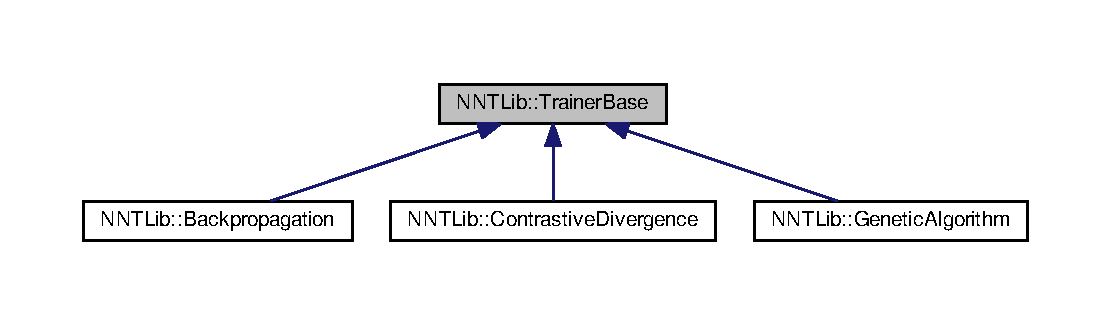
\includegraphics[width=350pt]{class_n_n_t_lib_1_1_trainer_base__inherit__graph}
\end{center}
\end{figure}


Collaboration diagram for N\+N\+T\+Lib\+:\+:Trainer\+Base\+:\nopagebreak
\begin{figure}[H]
\begin{center}
\leavevmode
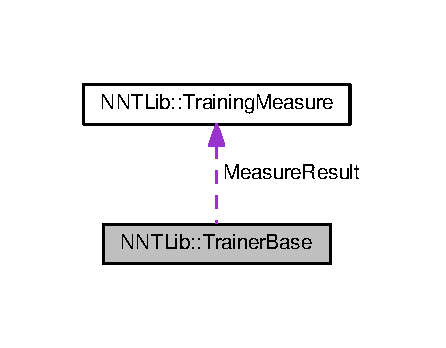
\includegraphics[width=214pt]{class_n_n_t_lib_1_1_trainer_base__coll__graph}
\end{center}
\end{figure}
\subsection*{Public Member Functions}
\begin{DoxyCompactItemize}
\item 
void \hyperlink{class_n_n_t_lib_1_1_trainer_base_ac048e1d40c13b919dc254559acf715e8}{Save\+Result} (std\+::string file, unsigned long long time\+Offset\+In\+Ms=0)
\begin{DoxyCompactList}\small\item\em Saves the mse result. \end{DoxyCompactList}\item 
\hyperlink{class_n_n_t_lib_1_1_trainer_base_a0b0d5fb69ec3526f9f1877d69a45f4f2}{Trainer\+Base} ()
\begin{DoxyCompactList}\small\item\em Initializes a new instance of the \hyperlink{class_n_n_t_lib_1_1_trainer_base}{Trainer\+Base} class. \end{DoxyCompactList}\item 
\hyperlink{class_n_n_t_lib_1_1_trainer_base_ac09e5c17c77cc5c76a896e1595a02f64}{$\sim$\+Trainer\+Base} ()
\begin{DoxyCompactList}\small\item\em Finalizes an instance of the \hyperlink{class_n_n_t_lib_1_1_trainer_base}{Trainer\+Base} class. \end{DoxyCompactList}\end{DoxyCompactItemize}
\subsection*{Public Attributes}
\begin{DoxyCompactItemize}
\item 
\hyperlink{struct_n_n_t_lib_1_1_training_measure}{Training\+Measure} $\ast$ \hyperlink{class_n_n_t_lib_1_1_trainer_base_a557584860d1e68175e6902b4095cefde}{Measure\+Result}
\begin{DoxyCompactList}\small\item\em The measure result \end{DoxyCompactList}\item 
int \hyperlink{class_n_n_t_lib_1_1_trainer_base_a7077caabdc27417bbb200537f6a8bcda}{Measure\+Result\+Lenght}
\begin{DoxyCompactList}\small\item\em The measure result lenght \end{DoxyCompactList}\item 
int \hyperlink{class_n_n_t_lib_1_1_trainer_base_a813093150b33e456c99428f2a4191c66}{Measure\+Filled\+Result\+Lenght}
\begin{DoxyCompactList}\small\item\em The measure filled result lenght \end{DoxyCompactList}\end{DoxyCompactItemize}
\subsection*{Protected Member Functions}
\begin{DoxyCompactItemize}
\item 
void \hyperlink{class_n_n_t_lib_1_1_trainer_base_a9fed2107d9f71064f7ca23eadcd67f2f}{init\+Measure\+Result} (int lenght)
\begin{DoxyCompactList}\small\item\em Initializes the measure result. \end{DoxyCompactList}\end{DoxyCompactItemize}


\subsection{Constructor \& Destructor Documentation}
\hypertarget{class_n_n_t_lib_1_1_trainer_base_a0b0d5fb69ec3526f9f1877d69a45f4f2}{}\index{N\+N\+T\+Lib\+::\+Trainer\+Base@{N\+N\+T\+Lib\+::\+Trainer\+Base}!Trainer\+Base@{Trainer\+Base}}
\index{Trainer\+Base@{Trainer\+Base}!N\+N\+T\+Lib\+::\+Trainer\+Base@{N\+N\+T\+Lib\+::\+Trainer\+Base}}
\subsubsection[{Trainer\+Base}]{\setlength{\rightskip}{0pt plus 5cm}N\+N\+T\+Lib\+::\+Trainer\+Base\+::\+Trainer\+Base (
\begin{DoxyParamCaption}
{}
\end{DoxyParamCaption}
)}\label{class_n_n_t_lib_1_1_trainer_base_a0b0d5fb69ec3526f9f1877d69a45f4f2}


Initializes a new instance of the \hyperlink{class_n_n_t_lib_1_1_trainer_base}{Trainer\+Base} class. 

\hypertarget{class_n_n_t_lib_1_1_trainer_base_ac09e5c17c77cc5c76a896e1595a02f64}{}\index{N\+N\+T\+Lib\+::\+Trainer\+Base@{N\+N\+T\+Lib\+::\+Trainer\+Base}!````~Trainer\+Base@{$\sim$\+Trainer\+Base}}
\index{````~Trainer\+Base@{$\sim$\+Trainer\+Base}!N\+N\+T\+Lib\+::\+Trainer\+Base@{N\+N\+T\+Lib\+::\+Trainer\+Base}}
\subsubsection[{$\sim$\+Trainer\+Base}]{\setlength{\rightskip}{0pt plus 5cm}N\+N\+T\+Lib\+::\+Trainer\+Base\+::$\sim$\+Trainer\+Base (
\begin{DoxyParamCaption}
{}
\end{DoxyParamCaption}
)}\label{class_n_n_t_lib_1_1_trainer_base_ac09e5c17c77cc5c76a896e1595a02f64}


Finalizes an instance of the \hyperlink{class_n_n_t_lib_1_1_trainer_base}{Trainer\+Base} class. 



\subsection{Member Function Documentation}
\hypertarget{class_n_n_t_lib_1_1_trainer_base_a9fed2107d9f71064f7ca23eadcd67f2f}{}\index{N\+N\+T\+Lib\+::\+Trainer\+Base@{N\+N\+T\+Lib\+::\+Trainer\+Base}!init\+Measure\+Result@{init\+Measure\+Result}}
\index{init\+Measure\+Result@{init\+Measure\+Result}!N\+N\+T\+Lib\+::\+Trainer\+Base@{N\+N\+T\+Lib\+::\+Trainer\+Base}}
\subsubsection[{init\+Measure\+Result}]{\setlength{\rightskip}{0pt plus 5cm}void N\+N\+T\+Lib\+::\+Trainer\+Base\+::init\+Measure\+Result (
\begin{DoxyParamCaption}
\item[{int}]{lenght}
\end{DoxyParamCaption}
)\hspace{0.3cm}{\ttfamily [protected]}}\label{class_n_n_t_lib_1_1_trainer_base_a9fed2107d9f71064f7ca23eadcd67f2f}


Initializes the measure result. 


\begin{DoxyParams}{Parameters}
{\em lenght} & The lenght.\\
\hline
\end{DoxyParams}
\hypertarget{class_n_n_t_lib_1_1_trainer_base_ac048e1d40c13b919dc254559acf715e8}{}\index{N\+N\+T\+Lib\+::\+Trainer\+Base@{N\+N\+T\+Lib\+::\+Trainer\+Base}!Save\+Result@{Save\+Result}}
\index{Save\+Result@{Save\+Result}!N\+N\+T\+Lib\+::\+Trainer\+Base@{N\+N\+T\+Lib\+::\+Trainer\+Base}}
\subsubsection[{Save\+Result}]{\setlength{\rightskip}{0pt plus 5cm}void N\+N\+T\+Lib\+::\+Trainer\+Base\+::\+Save\+Result (
\begin{DoxyParamCaption}
\item[{std\+::string}]{file, }
\item[{unsigned long long}]{time\+Offset\+In\+Ms = {\ttfamily 0}}
\end{DoxyParamCaption}
)}\label{class_n_n_t_lib_1_1_trainer_base_ac048e1d40c13b919dc254559acf715e8}


Saves the mse result. 


\begin{DoxyParams}{Parameters}
{\em file} & The file.\\
\hline
{\em time\+Offset\+In\+Ms} & The time offset in ms.\\
\hline
\end{DoxyParams}


\subsection{Member Data Documentation}
\hypertarget{class_n_n_t_lib_1_1_trainer_base_a813093150b33e456c99428f2a4191c66}{}\index{N\+N\+T\+Lib\+::\+Trainer\+Base@{N\+N\+T\+Lib\+::\+Trainer\+Base}!Measure\+Filled\+Result\+Lenght@{Measure\+Filled\+Result\+Lenght}}
\index{Measure\+Filled\+Result\+Lenght@{Measure\+Filled\+Result\+Lenght}!N\+N\+T\+Lib\+::\+Trainer\+Base@{N\+N\+T\+Lib\+::\+Trainer\+Base}}
\subsubsection[{Measure\+Filled\+Result\+Lenght}]{\setlength{\rightskip}{0pt plus 5cm}int N\+N\+T\+Lib\+::\+Trainer\+Base\+::\+Measure\+Filled\+Result\+Lenght}\label{class_n_n_t_lib_1_1_trainer_base_a813093150b33e456c99428f2a4191c66}


The measure filled result lenght 

\hypertarget{class_n_n_t_lib_1_1_trainer_base_a557584860d1e68175e6902b4095cefde}{}\index{N\+N\+T\+Lib\+::\+Trainer\+Base@{N\+N\+T\+Lib\+::\+Trainer\+Base}!Measure\+Result@{Measure\+Result}}
\index{Measure\+Result@{Measure\+Result}!N\+N\+T\+Lib\+::\+Trainer\+Base@{N\+N\+T\+Lib\+::\+Trainer\+Base}}
\subsubsection[{Measure\+Result}]{\setlength{\rightskip}{0pt plus 5cm}{\bf Training\+Measure}$\ast$ N\+N\+T\+Lib\+::\+Trainer\+Base\+::\+Measure\+Result}\label{class_n_n_t_lib_1_1_trainer_base_a557584860d1e68175e6902b4095cefde}


The measure result 

\hypertarget{class_n_n_t_lib_1_1_trainer_base_a7077caabdc27417bbb200537f6a8bcda}{}\index{N\+N\+T\+Lib\+::\+Trainer\+Base@{N\+N\+T\+Lib\+::\+Trainer\+Base}!Measure\+Result\+Lenght@{Measure\+Result\+Lenght}}
\index{Measure\+Result\+Lenght@{Measure\+Result\+Lenght}!N\+N\+T\+Lib\+::\+Trainer\+Base@{N\+N\+T\+Lib\+::\+Trainer\+Base}}
\subsubsection[{Measure\+Result\+Lenght}]{\setlength{\rightskip}{0pt plus 5cm}int N\+N\+T\+Lib\+::\+Trainer\+Base\+::\+Measure\+Result\+Lenght}\label{class_n_n_t_lib_1_1_trainer_base_a7077caabdc27417bbb200537f6a8bcda}


The measure result lenght 



The documentation for this class was generated from the following files\+:\begin{DoxyCompactItemize}
\item 
N\+N\+T\+Lib/Trainer\+Base.\+h\item 
N\+N\+T\+Lib/Trainer\+Base.\+cpp\end{DoxyCompactItemize}

\hypertarget{struct_n_n_t_lib_1_1_training_measure}{}\section{N\+N\+T\+Lib\+:\+:Training\+Measure Struct Reference}
\label{struct_n_n_t_lib_1_1_training_measure}\index{N\+N\+T\+Lib\+::\+Training\+Measure@{N\+N\+T\+Lib\+::\+Training\+Measure}}
\subsection*{Public Member Functions}
\begin{DoxyCompactItemize}
\item 
\hyperlink{struct_n_n_t_lib_1_1_training_measure_a4a3960c136ba4a48d425a5f42548be69}{Training\+Measure} ()
\begin{DoxyCompactList}\small\item\em Initializes a new instance of the \hyperlink{struct_n_n_t_lib_1_1_training_measure}{Training\+Measure} struct. \end{DoxyCompactList}\item 
\hyperlink{struct_n_n_t_lib_1_1_training_measure_accf24a164322c91ca64fce04c3bf7ee1}{$\sim$\+Training\+Measure} ()
\begin{DoxyCompactList}\small\item\em Finalizes an instance of the \hyperlink{struct_n_n_t_lib_1_1_training_measure}{Training\+Measure} class. \end{DoxyCompactList}\end{DoxyCompactItemize}
\subsection*{Public Attributes}
\begin{DoxyCompactItemize}
\item 
double \hyperlink{struct_n_n_t_lib_1_1_training_measure_a03470415cd36f35e43b3ad0e784bbbbf}{Mean\+Square\+Error}
\begin{DoxyCompactList}\small\item\em The mean square error \end{DoxyCompactList}\item 
unsigned long long \hyperlink{struct_n_n_t_lib_1_1_training_measure_abbe43852bac79bd5b7acfe6151464c37}{Execute\+Time}
\begin{DoxyCompactList}\small\item\em The execute time \end{DoxyCompactList}\end{DoxyCompactItemize}


\subsection{Constructor \& Destructor Documentation}
\hypertarget{struct_n_n_t_lib_1_1_training_measure_a4a3960c136ba4a48d425a5f42548be69}{}\index{N\+N\+T\+Lib\+::\+Training\+Measure@{N\+N\+T\+Lib\+::\+Training\+Measure}!Training\+Measure@{Training\+Measure}}
\index{Training\+Measure@{Training\+Measure}!N\+N\+T\+Lib\+::\+Training\+Measure@{N\+N\+T\+Lib\+::\+Training\+Measure}}
\subsubsection[{Training\+Measure}]{\setlength{\rightskip}{0pt plus 5cm}N\+N\+T\+Lib\+::\+Training\+Measure\+::\+Training\+Measure (
\begin{DoxyParamCaption}
{}
\end{DoxyParamCaption}
)}\label{struct_n_n_t_lib_1_1_training_measure_a4a3960c136ba4a48d425a5f42548be69}


Initializes a new instance of the \hyperlink{struct_n_n_t_lib_1_1_training_measure}{Training\+Measure} struct. 

\hypertarget{struct_n_n_t_lib_1_1_training_measure_accf24a164322c91ca64fce04c3bf7ee1}{}\index{N\+N\+T\+Lib\+::\+Training\+Measure@{N\+N\+T\+Lib\+::\+Training\+Measure}!````~Training\+Measure@{$\sim$\+Training\+Measure}}
\index{````~Training\+Measure@{$\sim$\+Training\+Measure}!N\+N\+T\+Lib\+::\+Training\+Measure@{N\+N\+T\+Lib\+::\+Training\+Measure}}
\subsubsection[{$\sim$\+Training\+Measure}]{\setlength{\rightskip}{0pt plus 5cm}N\+N\+T\+Lib\+::\+Training\+Measure\+::$\sim$\+Training\+Measure (
\begin{DoxyParamCaption}
{}
\end{DoxyParamCaption}
)}\label{struct_n_n_t_lib_1_1_training_measure_accf24a164322c91ca64fce04c3bf7ee1}


Finalizes an instance of the \hyperlink{struct_n_n_t_lib_1_1_training_measure}{Training\+Measure} class. 



\subsection{Member Data Documentation}
\hypertarget{struct_n_n_t_lib_1_1_training_measure_abbe43852bac79bd5b7acfe6151464c37}{}\index{N\+N\+T\+Lib\+::\+Training\+Measure@{N\+N\+T\+Lib\+::\+Training\+Measure}!Execute\+Time@{Execute\+Time}}
\index{Execute\+Time@{Execute\+Time}!N\+N\+T\+Lib\+::\+Training\+Measure@{N\+N\+T\+Lib\+::\+Training\+Measure}}
\subsubsection[{Execute\+Time}]{\setlength{\rightskip}{0pt plus 5cm}unsigned long long N\+N\+T\+Lib\+::\+Training\+Measure\+::\+Execute\+Time}\label{struct_n_n_t_lib_1_1_training_measure_abbe43852bac79bd5b7acfe6151464c37}


The execute time 

\hypertarget{struct_n_n_t_lib_1_1_training_measure_a03470415cd36f35e43b3ad0e784bbbbf}{}\index{N\+N\+T\+Lib\+::\+Training\+Measure@{N\+N\+T\+Lib\+::\+Training\+Measure}!Mean\+Square\+Error@{Mean\+Square\+Error}}
\index{Mean\+Square\+Error@{Mean\+Square\+Error}!N\+N\+T\+Lib\+::\+Training\+Measure@{N\+N\+T\+Lib\+::\+Training\+Measure}}
\subsubsection[{Mean\+Square\+Error}]{\setlength{\rightskip}{0pt plus 5cm}double N\+N\+T\+Lib\+::\+Training\+Measure\+::\+Mean\+Square\+Error}\label{struct_n_n_t_lib_1_1_training_measure_a03470415cd36f35e43b3ad0e784bbbbf}


The mean square error 



The documentation for this struct was generated from the following files\+:\begin{DoxyCompactItemize}
\item 
N\+N\+T\+Lib/Training\+Measure.\+h\item 
N\+N\+T\+Lib/Training\+Measure.\+cpp\end{DoxyCompactItemize}

%--- End generated contents ---

% Index
\backmatter
\newpage
\phantomsection
\clearemptydoublepage
\addcontentsline{toc}{chapter}{Index}
\printindex

\end{document}
